%\documentclass[catalan,a4paper,11pt,openright,final]{book}
%\documentclass[catalan,a4paper,11pt,oneside,final]{book}
\documentclass[catalan,a4paper,11pt,twoside,openright,final]{book}
\usepackage[main=catalan,english]{babel}
\usepackage[utf8]{inputenc}
\usepackage[T1]{fontenc}
\usepackage{lmodern}
\usepackage{graphicx}
\usepackage{amsmath}
\usepackage{amssymb}
\usepackage{amsthm}
\usepackage{fancyhdr}
\usepackage{xcolor}
\usepackage{multirow}
\usepackage{chngcntr}
\usepackage{booktabs}
\usepackage{longtable}
\usepackage{tabularx}
\usepackage{array}
\usepackage{enumitem}
\usepackage{float}
\usepackage{caption}
\usepackage{subcaption}
\usepackage{url}
\usepackage[numbers,sort&compress]{natbib}
\usepackage[hidelinks]{hyperref}
\usepackage{microtype}
%%\usepackage{subeqnarray}

\sloppy    %% Alinea el texte reduint el nombre de paraules trencades amb guions
%\pagestyle{headings}
%\parskip 10pt
\setlength{\parskip}{1.5ex}
\setlength{\topmargin}{-0.75cm}
\setlength{\oddsidemargin}{0.5cm}
%\setlength{\evensidemargin}{0.5cm}
\setlength{\evensidemargin}{-0.58cm} %
\setlength{\textwidth}{16cm} \setlength{\textheight}{23cm}
\renewcommand{\baselinestretch}{1.25} \small\normalsize

\renewcommand{\qedsymbol}{$\blacksquare$}
% STANDARD NEW COMMAND DEFINITIONS
\newtheorem{lemma}{\textbf{Lemma}}
\renewcommand{\v}[1]{\mathbf{#1}}
\newcommand{\eq}[1]{\begin{equation}{#1}\end{equation}}
\newcommand{\p}[1]{\left(#1\right)}
\newcommand{\corch}[1]{\left[#1\right]}
\newcommand{\llav}[1]{\left\{#1\right\}}
% CURRENT PAPER SPECIFIC NEW COMMAND DEFINITIONS
\DeclareMathSymbol{\Re}{\mathbin}{AMSb}{"52}
\DeclareMathSymbol{\Ce}{\mathbin}{AMSb}{"43}
\DeclareMathSymbol{\F}{\mathbin}{AMSb}{"46}
\DeclareMathSymbol{\G}{\mathbin}{AMSb}{"47}

\newcommand{\code}[1]{\texttt{#1}}
\newcommand{\unit}[1]{\,\mathrm{#1}}
\newcommand{\bps}{\mathrm{bit}\,\mathrm{px}^{-1}\,\mathrm{band}^{-1}}
\newcommand{\dataset}[1]{\textit{#1}}
\newcommand{\sourcepath}[1]{\texttt{\detokenize{#1}}}
\newcommand{\figsource}[1]{\par\smallskip{\footnotesize\textit{Font:} #1}}
\newcommand{\etal}{\textit{et al.}}
\graphicspath{{figures/}}
\counterwithout{figure}{chapter}
\counterwithout{table}{chapter}


\setlength{\unitlength}{1mm}

\pagestyle{fancy} %xx
\setlength{\headheight}{14pt}
\fancyhead[LE,RO]{\thepage} %
\fancyhead[RE]{\nouppercase \leftmark} %
\fancyhead[LO]{\nouppercase \rightmark} %
\fancyhead[CF]{} %
%\renewcommand{\headrulewidth}{0.4pt}

%\include{macros}
\begin{document}
\selectlanguage{catalan}
%
% =================================================================
% Front matter
% =================================================================
%
\hypersetup{pageanchor=false}
% !TEX root = main.tex
\begin{titlepage}
\begin{center}

\renewcommand{\baselinestretch}{1.0} \small\normalsize




\includegraphics[width=6.5cm]{logoUAB.jpg}\\
\vspace{2cm}
{\normalsize {\sc Treball de Fi de Grau}\\}
\vspace{0.5cm}
{\normalsize {\sc Grau en Enginyeria de Sistemes de Telecomunicació}\\}
\vspace{3cm}
{\huge\sc Implementació de compressió a qualitat fixa per a dades de satèl·lit multiespectrals}\\[0.8cm]
\vspace{1.7cm} {\Large Cristhian Omar Añez López} \\
\vspace{5.5cm}


{\normalsize {\sc Director:} Sebastià Mijares Verdú\\
\vspace{0.25cm}
{\sc Departament de Telecomunicació i Enginyeria de Sistemes}\\
\vspace{0.25cm}
{\sc Universitat Autònoma de Barcelona}\\}
\vspace{0.75cm}
{\normalsize Bellaterra, 29 de juliol de 2026}

\end{center}
\end{titlepage}

\thispagestyle{empty} %
\cleardoublepage %
\pagenumbering{roman}
\hypersetup{pageanchor=true}

% !TEX root = main.tex
\chapter*{Abstract\label{Abstract}}
\addcontentsline{toc}{chapter}{Abstract}
\fancyhead[RE]{\slshape \textsf{Abstract}} %
\fancyhead[LO]{\slshape \textsf{Abstract}} %

\begin{otherlanguage*}{english}

Earth-observation satellites acquire increasing volumes of multispectral data
under constraints on downlink capacity, memory, and on-board processing. This
thesis implements the compression and decompression pipeline of SORTENY, a
neural multispectral image codec, in C and extends it with spatial quality
control that does not require manual selection of regions of interest.

Quality is assigned block-wise through maps generated automatically from the
spectral and spatial content of the image. Detectors identify priority blocks,
and quality policies determine how fidelity is distributed between those
blocks and the background. Two complementary strategies were studied: one
prioritizes bit savings by degrading non-priority regions, whereas the other
assigns a fixed high quality to the detected region to favor its preservation.

The evaluation included 120 eight-band Sentinel-2 crops. The coded bitrate was
subsequently measured with the reference pipeline on 20 selected crops. The
bit-saving strategy reduced the mean bitrate by 8.84\% relative to applying
uniform quality to the whole image, while maintaining or slightly improving
fidelity in the prioritized regions and concentrating degradation in the
background. The preservation strategy protected those regions further at the
cost of a smaller bitrate reduction.

The C implementation was also evaluated on a Raspberry Pi 3B+ as a
representative resource-constrained platform. Relative to the initial C version
running with the same four threads, the introduced optimizations reduced mean
total runtime by 17.0\%, equivalent to a $1.205\times$ speed-up, with no
detected functional changes or relevant increase in memory use. Automatic
quality-map generation accounted for less than 0.05\% of the codec runtime.
Therefore, spatial decision has negligible cost, and neural codec execution
remains the main bottleneck. The current C bitstream still lacks the final
entropy or arithmetic coder. The Raspberry is used as a computational proxy
for a resource-constrained on-board platform; validation on the final hardware
of a specific mission remains outside the scope of this work.

\textbf{Keywords:} multispectral image compression, learned compression,
fixed-quality compression, region of interest, on-board processing, embedded
systems, Raspberry Pi, quality map.

\end{otherlanguage*}

\thispagestyle{empty}
\cleardoublepage

% !TEX root = main.tex
\chapter*{Resum\label{Resum}}
\addcontentsline{toc}{chapter}{Resum}
\fancyhead[RE]{\slshape \textsf{Resum}} %
\fancyhead[LO]{\slshape \textsf{Resum}} %

Els satèl·lits d'observació de la Terra adquireixen volums creixents de dades
multiespectrals sota restriccions d'enllaç de baixada, memòria i processament a
bord. Aquesta memòria implementa en C el pipeline de compressió i descompressió
de SORTENY, un còdec neuronal d'imatges multiespectrals, i l'estén amb control
espacial de qualitat sense selecció manual de regions d'interès.

La qualitat s'assigna per blocs mitjançant mapes generats automàticament a partir
del contingut espectral i espacial de la imatge. Els detectors identifiquen els
blocs prioritaris i les polítiques de qualitat decideixen com es distribueix la
fidelitat entre aquests blocs i el fons. S'han estudiat dues estratègies
complementàries: una prioritza l'estalvi de bits degradant les regions no
prioritàries, i l'altra fixa una qualitat alta dins la regió detectada per
afavorir-ne la conservació.

L'avaluació va incloure 120 retalls Sentinel-2 de vuit bandes. El bitrate
codificat es va mesurar posteriorment amb el pipeline de referència sobre 20
retalls seleccionats. L'estratègia orientada a l'estalvi va reduir el bitrate
mitjà un 8,84\% respecte d'aplicar una qualitat uniforme a tota la imatge,
mentre mantenia o millorava lleugerament la fidelitat de les regions
prioritzades i concentrava la degradació al fons. L'estratègia de preservació va
protegir més aquestes regions a canvi d'un estalvi menor.

La implementació C també es va avaluar en una Raspberry Pi 3B+ com a plataforma
representativa de recursos limitats. Respecte de la versió C inicial executada
amb els mateixos quatre fils, les optimitzacions van reduir el temps total
mitjà un 17,0\%, equivalent a una acceleració d'$1,205\times$, sense canvis
funcionals detectats ni un augment rellevant de memòria. La generació automàtica
del mapa de qualitat va representar menys del 0,05\% del temps del còdec. Per
tant, la decisió espacial té un cost negligible i el principal coll d'ampolla
és l'execució del còdec neuronal. Com a limitacions, el flux binari C encara no
incorpora el codificador final per entropia o aritmètic. La Raspberry s'utilitza
com a referència computacional d'una plataforma a bord de baix recurs; la
validació sobre el hardware definitiu d'una missió queda fora de l'abast.

\textbf{Paraules clau:} compressió d'imatges multiespectrals, compressió
apresa, qualitat fixa, regió d'interès, processament a bord, sistemes encastats,
Raspberry Pi, mapa de qualitat.

\thispagestyle{empty}
\cleardoublepage


\renewcommand{\baselinestretch}{1.25}
\fancyhead[RE]{\slshape \textsf{Índex}}
\fancyhead[LO]{\slshape \textsf{Índex}}
\tableofcontents
\cleardoublepage
\thispagestyle{empty}

\fancyhead[RE]{\slshape \textsf{Llista de figures}}
\fancyhead[LO]{\slshape \textsf{Llista de figures}}
\listoffigures
\addcontentsline{toc}{chapter}{Llista de figures}
\cleardoublepage
\thispagestyle{empty}

\listoftables
\addcontentsline{toc}{chapter}{Llista de taules}
\fancyhead[RE]{\slshape \textsf{Llista de taules}}
\fancyhead[LO]{\slshape \textsf{Llista de taules}}
\thispagestyle{empty}
\cleardoublepage

% !TEX root = main.tex
\chapter*{Sigles i notació\label{Acronyms}}
\addcontentsline{toc}{chapter}{Sigles i notació}
\fancyhead[RE]{\slshape \textsf{Sigles i notació}}
\fancyhead[LO]{\slshape \textsf{Sigles i notació}}

\begin{longtable}{>{\bfseries}p{2.7cm}p{11.8cm}}
ARM & Arquitectura de processadors \textit{Advanced RISC Machines}. \\
bps & Bits per mostra espectral; en aquesta memòria, $\bps$, equivalent a bits
per píxel i banda. \\
CCSDS & \textit{Consultative Committee for Space Data Systems}. \\
CSMR & Implementació de referència del mètode neuronal de compressió
multiràtio i qualitat fixa emprada per generar fitxers \code{.tfci}. \\
DWT & \textit{Discrete Wavelet Transform}. \\
GDN/IGDN & \textit{Generalized Divisive Normalization} i transformada inversa. \\
MSE & \textit{Mean Squared Error}, error quadràtic mitjà. \\
NDVI & \textit{Normalized Difference Vegetation Index}. \\
NDWI & \textit{Normalized Difference Water Index}. \\
OBC & \textit{On-Board Computer}. \\
OpenMP & Interfície de programació per paral·lelisme de memòria compartida. \\
PSNR & \textit{Peak Signal-to-Noise Ratio}. \\
Q-map & Matriu de valors $Q$ que assigna una qualitat a cada bloc espacial. \\
ROI & \textit{Region of Interest}, regió d'interès. \\
RSS & \textit{Resident Set Size}, memòria resident màxima del procés. \\
SWIR & Infraroig d'ona curta. \\
TFC & \textit{TensorFlow Compression}. \\
VAE & \textit{Variational Autoencoder}. \\
\end{longtable}

\thispagestyle{empty}
\cleardoublepage

\setlength{\parskip}{1.5ex}

%
% =================================================================
% Contents
% =================================================================
%
\setcounter{chapter}{0} \pagenumbering{arabic}
\setcounter{figure}{0}
\setcounter{table}{0}
\newcounter{one_two_three}
\newcounter{appcnt}[chapter]
\newcounter{pastchapter}[chapter]
\newcounter{pastchapter2}[chapter]

\setcounter{tocdepth}{2}     % -1 = Part         0 = Chapter    1 = Section       2 = Subsection
\setcounter{secnumdepth}{3}  % 3 = Subsubsection 4 = Paragraph  5 = Subparagraph

\setlength{\parskip}{1.5ex}
\renewcommand{\arraystretch}{1.25}


\cleardoublepage
% !TEX root = ../main.tex
\chapter{Introducció}\label{ch:introduccio}
\fancyhead[RE]{\slshape \textsf{Capítol \thechapter.\ Introducció}}
\fancyhead[LO]{\slshape \textsf{\nouppercase \rightmark}}

\section{Context i motivació}\label{sec:context}

Els instruments d'observació de la Terra produeixen imatges amb una resolució
espacial, espectral i temporal cada vegada més elevada. Aquest increment
millora la capacitat de caracteritzar vegetació, aigua, sòl, atmosfera o
infraestructures, però també augmenta el volum que cal emmagatzemar i
transmetre. En una missió espacial, la capacitat de l'enllaç de baixada no
creix necessàriament al mateix ritme que el sensor. Per tant, la compressió no
és únicament una etapa posterior de tractament de dades: condiciona quantes
imatges poden adquirir-se, conservar-se i enviar-se durant la vida de la
missió \cite{blanes2014tutorial,bioucas2013hyperspectral,denis2017disruptions}.

El problema s'accentua en nanosatèl·lits i altres plataformes amb recursos
limitats. La memòria, la potència elèctrica, la capacitat de càlcul i el temps
de contacte amb les estacions de terra són restriccions simultànies
\cite{selva2012cubesats,nasa2017cubesat}. Comprimir a terra no resol aquesta
situació, perquè les dades crues ja han hagut de travessar l'enllaç. La decisió
s'ha de prendre a bord, abans de transmetre.

Els estàndards CCSDS ofereixen solucions consolidades per a compressió sense
pèrdues, amb pèrdues i gairebé sense pèrdues
\cite{ccsds121,ccsds122,ccsds1221,ccsds123}. Paral·lelament, els còdecs basats
en xarxes neuronals han demostrat una gran capacitat per aprendre transformades
adaptades a les dades i obtenir bons compromisos entre la mida codificada i la
qualitat de reconstrucció
\cite{balle2017end,balle2018hyperprior,mijares2023reduced}. SORTENY parteix
d'aquesta segona línia: combina transformades espectrals i espacials apreses
per comprimir imatges multiespectrals \cite{mijares2025sorteny}.

\section{Antecedent propi i problema pendent}\label{sec:antecedent_intro}

Aquest treball continua un desenvolupament propi anterior que va adaptar el
compressor de referència de SORTENY, escrit en Python i TensorFlow, a una
implementació nativa en C \cite{anez2026treball}. Aquell desenvolupament va
exportar els pesos entrenats a fitxers consumibles des de C, va implementar els
operadors de la transformada d'anàlisi i va reduir l'ús de memòria mitjançant la
reutilització de buffers. També va introduir paral·lelisme i va executar el
compressor en una Raspberry Pi 3B+.

En una imatge de prova, la versió C va reduir la memòria màxima aproximadament
un factor $9,2\times$ i va accelerar l'execució $1,47\times$ respecte de la
referència Python. Aquests resultats demostraven que la inferència del
compressor podia traslladar-se a una plataforma amb menys d'un gigabyte de
memòria, però no constituïen encara un còdec complet.

Partint d'aquell resultat, quedaven cinc problemes oberts: completar la
reconstrucció en C; fer que el fitxer generat pel compressor inclogués tot el
que el descompressor necessita per reconstruir la imatge, sense dades auxiliars
externes; permetre qualitats diferents dins d'una mateixa imatge; decidir
automàticament quines regions cal protegir; i mesurar tant la mida real de les
dades codificades com el cost computacional del sistema complet. Aquests
problemes defineixen el punt de partida de la memòria actual.

\section{Problema i preguntes de recerca}\label{sec:problema}

Un còdec de qualitat uniforme assigna el mateix compromís de distorsió a tota
la imatge. Aquesta decisió és senzilla i reproduïble, però ignora que una
escena pot contenir zones amb valors operatius diferents. En una aplicació de
seguiment de vegetació pot interessar conservar millor les zones vegetades i
acceptar més distorsió a la resta. En una adquisició afectada per núvols pot
ser preferible dedicar més dades a les zones no cobertes per núvols, on la
superfície continua sent observable.

La selecció manual de regions és útil com a instrument experimental, però no
és una solució operativa general. Un satèl·lit no disposa d'un operador que
inspeccioni cada imatge abans de comprimir-la. Per tant, el sistema ha de
resoldre automàticament dues decisions diferents: identificar quines regions
són d'interès i determinar quina qualitat s'assigna a aquestes regions i a la
resta de la imatge. Separar les dues decisions permet canviar el criteri
d'interès sense redissenyar el còdec.

La recerca s'articula al voltant de quatre preguntes:

\begin{enumerate}[label=\textbf{P\arabic*.},leftmargin=*]
  \item Es pot completar i validar en C el procés de compressió i reconstrucció
  de SORTENY?
  \item Es poden identificar automàticament regions útils sense intervenció
  manual per a cada imatge?
  \item Es pot reduir la mida codificada redistribuint la qualitat sense
  perjudicar la regió que es vol protegir?
  \item És assumible el cost d'aquesta decisió i del còdec complet en una
  plataforma amb recursos limitats?
\end{enumerate}

Les hipòtesis mesurables associades a aquestes preguntes es formulen al
Capítol~\ref{ch:metodologia}, una vegada definits el sistema, les magnituds i
els criteris experimentals.

\section{Objectius}\label{sec:objectius}

L'objectiu general és completar i avaluar una extensió en C de SORTENY capaç
d'assignar automàticament qualitats diferents a regions d'una imatge
multiespectral i d'executar-se en maquinari amb recursos limitats.

Els objectius específics són:

\begin{enumerate}[label=\textbf{O\arabic*.},leftmargin=*]
  \item Completar i validar el compressor i el descompressor C respecte del
  comportament esperat del model de referència.
  \item Automatitzar la identificació de regions d'interès i l'assignació
  espacial de qualitat, sense requerir una selecció manual per imatge.
  \item Mesurar el compromís entre mida codificada i qualitat de reconstrucció
  respecte d'una compressió uniforme.
  \item Optimitzar les operacions C de més cost, conservar el comportament
  funcional i mesurar temps i memòria en una Raspberry Pi.
  \item Determinar en quines condicions l'estalvi de transmissió compensa el
  càlcul addicional i identificar les limitacions que encara impedeixen una
  adopció operativa completa.
\end{enumerate}

\section{Abast del treball}\label{sec:abast}

L'avaluació utilitza imatges multiespectrals de vuit bandes i una
implementació C executada tant en un entorn local com en una Raspberry Pi 3B+.
El treball no entrena un nou model neuronal: parteix dels pesos existents i es
centra a completar el còdec, controlar espacialment la qualitat i validar-ne
el comportament. La mida codificada final es mesura amb el codificador de la
implementació de referència; el flux C actual s'avalua separadament i encara no
incorpora aquesta etapa final de codificació.

La Raspberry Pi s'utilitza com una plataforma representativa de baix recurs,
útil per mesurar memòria, paral·lelisme i colls d'ampolla. L'existència de
plataformes a bord amb tecnologies COTS i prestacions comparables, com C3SatP a
la missió Menut, justifica l'interès de la comparació
\cite{schwaller2017a53,serra2024c3satp}. No obstant això, aquesta prova no
constitueix una qualificació de vol: no avalua radiació, consum energètic amb
instrumentació externa, fiabilitat de missió ni temps real per a un sensor
concret.

\section{Metodologia i organització}\label{sec:metodologia_organitzacio}

El desenvolupament s'ha realitzat de manera incremental. Abans de cada canvi
s'ha fixat una referència; després s'ha modificat un component aïllat i s'han
comparat els artefactes resultants. Una modificació només s'ha acceptat quan
les proves funcionals, les reconstruccions i les mesures associades han
confirmat el comportament esperat. Les proves de major cost s'han reservat per
als candidats que ja havien superat comprovacions més curtes.

El Capítol~\ref{ch:estat_art} presenta les fonts, els estàndards i les
alternatives considerades. El Capítol~\ref{ch:fonaments} introdueix els
fonaments de compressió i qualitat necessaris. Els Capítols~\ref{ch:pipeline}
i~\ref{ch:control} descriuen l'evolució del pipeline C i el control espacial.
El Capítol~\ref{ch:metodologia} formalitza les hipòtesis i el disseny
experimental. Els Capítols~\ref{ch:resultats} i~\ref{ch:bord} presenten els
resultats de qualitat, compressió i execució en hardware limitat. Finalment,
el Capítol~\ref{ch:conclusions} respon les preguntes de recerca, comprova els
objectius i delimita el treball futur.

\thispagestyle{empty}

\cleardoublepage
% !TEX root = ../main.tex
\chapter{Estat de l'art i context tecnològic}\label{ch:estat_art}
\fancyhead[RE]{\slshape \textsf{Capítol \thechapter.\ Estat de l'art}}
\fancyhead[LO]{\slshape \textsf{\nouppercase \rightmark}}

Aquest capítol situa el treball en el context de la compressió d'imatges
d'observació de la Terra. Primer es presenten els requisits generals de la
compressió multiespectral i els estàndards espacials CCSDS, amb especial
atenció a CCSDS~122 perquè és el referent clàssic més proper a SORTENY.
Després s'introdueixen els còdecs neuronals, el model SORTENY, el concepte de
qualitat fixa i l'ús de regions d'interès. El capítol es tanca amb les
restriccions d'execució a bord i amb el buit pràctic que motiva la contribució
d'aquesta memòria.

\section{Criteri de revisió bibliogràfica}\label{sec:cerca}

La cerca d'informació s'ha organitzat al voltant de quatre blocs: compressió
espacial clàssica, compressió apresa, control de qualitat local i processament
a bord. S'han prioritzat fonts primàries o oficials: recomanacions CCSDS,
normes ISO/IEC i ECSS, articles revisats per parells, documentació de missions
i documentació tècnica dels fabricants. Quan s'han utilitzat fonts de context,
com fitxes de hardware o informació institucional de missions, no s'han emprat
per derivar xifres experimentals pròpies.

La revisió no pretén enumerar totes les variants existents. Cada referència
s'ha inclòs perquè aporta una definició, una alternativa tècnica, un mètode
comparable o una restricció de disseny. Les xifres experimentals pròpies, en
canvi, no depenen de la bibliografia: es vinculen a checkpoints i manifests del
projecte. Aquesta separació evita confondre resultats de tercers amb resultats
generats durant aquesta memòria. El treball previ propi s'utilitza com a
antecedent publicat en línia i es cita explícitament quan se'n reutilitza una
idea, una figura o una comparació \cite{anez2026treball}.

\section{Compressió d'imatges d'observació de la Terra}\label{sec:compressio_remota}

Una imatge multiespectral es pot escriure com un tensor
$\mathbf{x}\in\mathbb{R}^{B\times H\times W}$, on $B$ és el nombre de bandes
espectrals, $H$ l'alçada i $W$ l'amplada. La compressió intenta reduir la mida
del fitxer aprofitant dues redundàncies principals: la redundància espacial
entre píxels propers i la redundància espectral entre bandes correlacionades.
En imatges hiperespectrals, on el nombre de bandes pot ser molt més gran, la
redundància espectral és encara més important \cite{bioucas2013hyperspectral,
guanter2015enmap}.

Hi ha tres règims habituals. La compressió sense pèrdues reconstrueix
exactament les mostres originals, però l'estalvi queda limitat per l'entropia
de la font \cite{cover2006information,sayood2017compression}. La compressió
gairebé sense pèrdues introdueix un error acotat. La compressió amb pèrdues
accepta una distorsió més gran a canvi d'una reducció de dades superior. En
observació de la Terra no hi ha una resposta universal: depèn de la missió, del
sensor, de la calibració i de la tasca científica posterior
\cite{blanes2014tutorial,gonzalez2025robustness}.

Per comparar resultats en imatges multiespectrals, aquesta memòria expressa la
taxa en bits per píxel i per banda:

\begin{equation}
R_{\mathrm{bps}} =
\frac{8\,S_{\mathrm{fitxer}}}{HWB},
\label{eq:bps_intro}
\end{equation}

on $S_{\mathrm{fitxer}}$ és la mida comprimida en bytes. Per tant, \emph{bps}
no vol dir bits per segon en aquest document, sinó bits per mostra espacial i
per banda espectral. Quan es parla de velocitat temporal, s'utilitza
\emph{throughput} o temps d'execució.

JPEG~2000 és una referència general de compressió d'imatge fixa amb i sense
pèrdues \cite{iso15444}. Tot i això, les missions espacials solen prendre com
a punt de partida les recomanacions CCSDS, perquè estan pensades per
interoperabilitat, implementació embarcada i fluxos de dades d'instruments.

\section{Estàndards CCSDS}\label{sec:ccsds}

El Consultative Committee for Space Data Systems (CCSDS) defineix
recomanacions utilitzades en missions espacials. En compressió d'imatges i
dades multiespectrals, tres famílies són especialment rellevants: CCSDS~121,
CCSDS~122 i CCSDS~123.

\subsection{CCSDS 121 i CCSDS 123 com a context}

CCSDS~121 defineix compressió sense pèrdues per a dades d'instruments. Combina
un preprocessament opcional amb codis adaptatius, com els codis Rice, i prioritza
descodificació exacta i baixa complexitat \cite{ccsds121}. És molt útil com a
etapa de codificació per entropia o com a referència de robustesa, però no
defineix per si mateix una transformada espacial amb pèrdues.

CCSDS~123 està orientat a imatges multiespectrals i hiperespectrals. Es basa en
predicció: estima el valor d'una mostra a partir del veïnatge espacial i
espectral, i després codifica el residu \cite{ccsds123}. La versió B-2 permet
funcionament sense pèrdues o gairebé sense pèrdues i diferents codificadors per
entropia \cite{blanes2019parameter,kiely2018new}. Existeixen implementacions
paral·leles i hardware accelerat \cite{bascones2017parallel,barrios2021hls,
johansen2018fpga}, i arquitectures com SHyLoC mostren la maduresa de la línia
CCSDS en entorns espacials \cite{barrios2020shyloc}.

Tot i aquesta rellevància, CCSDS~123 no és el referent principal per situar
aquesta memòria, perquè SORTENY és un compressor amb pèrdues basat en
transformades apreses, no un predictor near-lossless. Per això el punt de
referència conceptual més proper és CCSDS~122.

\subsection{CCSDS 122 com a referent clàssic}

CCSDS~122 és una recomanació d'imatge basada en transformada. La seva estructura
general es pot veure a la Figura~\ref{fig:ccsds122_pipeline}: primer s'aplica
una transformada discreta d'ondeletes (DWT) i després un codificador de plans de
bits (BPE) genera el flux codificat \cite{ccsds122}.

\begin{figure}[H]
\centering
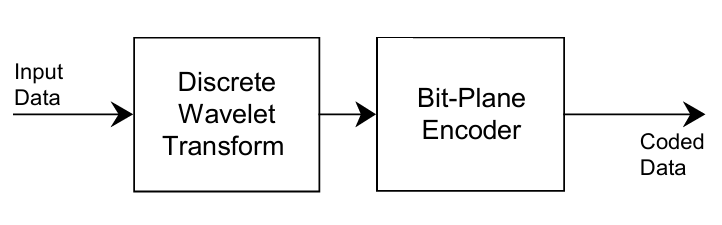
\includegraphics[width=0.72\textwidth]{ch2/ccsds122_pipeline.png}
\caption{Estructura general de CCSDS~122: transformada DWT seguida d'un codificador de plans de bits.}
\label{fig:ccsds122_pipeline}
\figsource{Adaptat del treball previ propi \cite{anez2026treball}.}
\end{figure}

La DWT separa la imatge en subbandes de baixa i alta freqüència. Aplicada de
forma separable, primer filtra files i després columnes, generant components
com $LL$, $LH$, $HL$ i $HH$. CCSDS~122 pot utilitzar filtres 5/3 enters per a
compressió reversible o filtres 9/7 biortogonals per a compressió amb pèrdues.
La transformada es pot aplicar recursivament sobre la subbanda $LL$, formant
una piràmide multiresolució com la de la Figura~\ref{fig:ccsds122_dwt}.

\begin{figure}[H]
\centering
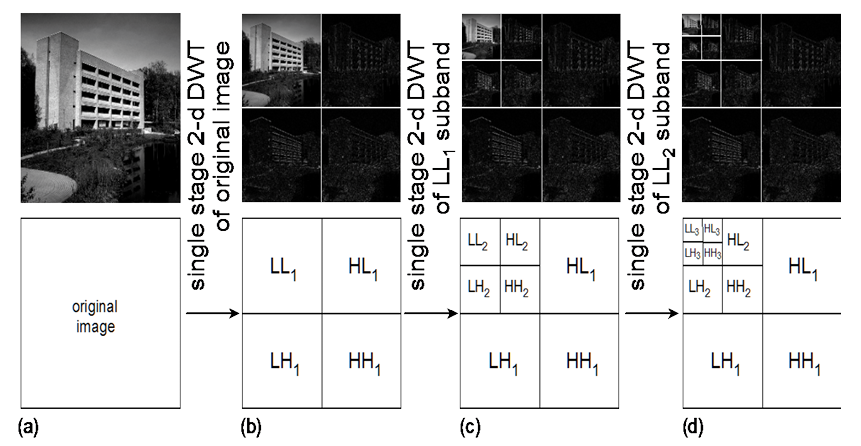
\includegraphics[width=0.82\textwidth]{ch2/ccsds122_dwt_multilevel.png}
\caption{Descomposició multiresolució amb DWT. La subbanda $LL$ concentra la informació de baixa freqüència i es pot tornar a descompondre.}
\label{fig:ccsds122_dwt}
\figsource{Adaptat del treball previ propi \cite{anez2026treball}.}
\end{figure}

El BPE codifica els coeficients transformats per plans de bits. Els bits més
significatius es codifiquen abans que els menys significatius, de manera que el
flux pot truncar-se i encara permet reconstruir una imatge completa amb menys
qualitat. A més, l'estructura d'arbres entre coeficients pare i fills en les
subbandes wavelet permet explotar que, si un coeficient de baixa freqüència és
poc significatiu, sovint també ho són els seus descendents
\cite{poupat2013cwicom}. Aquesta relació es resumeix a la
Figura~\ref{fig:ccsds122_family}.

\begin{figure}[H]
\centering
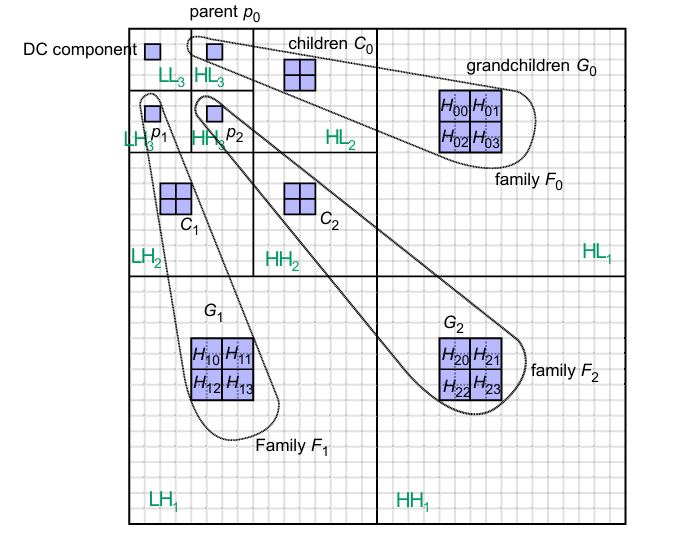
\includegraphics[width=0.55\textwidth]{ch2/ccsds122_wavelet_family.png}
\caption{Exemple de relació familiar entre coeficients wavelet utilitzada pel BPE.}
\label{fig:ccsds122_family}
\figsource{Adaptat del treball previ propi \cite{anez2026treball}.}
\end{figure}

CCSDS~122 és, per tant, un referent exigent: és madur, interpretable, ràpid i
orientat a implementacions embarcades. En el treball previ propi es va utilitzar
com a comparador experimental per situar el cost i la qualitat de SORTENY C
\cite{anez2026treball}. En aquesta memòria no es repeteix aquella comparativa:
CCSDS~122 es manté com a referència tecnològica de còdec espacial clàssic,
mentre que els experiments se centren en una pregunta diferent: com controlar
espacialment la qualitat dins de SORTENY i quin cost té fer-ho en C.

\section{Compressió apresa i SORTENY}\label{sec:learned}

\subsection{Autoencoders i models taxa--distorsió}

Els còdecs apresos parteixen d'una idea similar a la dels còdecs clàssics:
transformar la imatge a un domini on sigui més fàcil eliminar redundància,
quantitzar i reconstruir. La diferència és que la transformada no es defineix
manualment, com la DWT de CCSDS~122, sinó que s'aprèn a partir de dades. En la
forma bàsica, una transformada d'anàlisi $g_a$ produeix latents
$\mathbf{y}$, aquests latents es quantitzen, i una transformada de síntesi
$g_s$ reconstrueix la imatge:

\begin{equation}
\mathbf{y}=g_a(\mathbf{x}), \qquad
\hat{\mathbf{y}}=Q(\mathbf{y}), \qquad
\hat{\mathbf{x}}=g_s(\hat{\mathbf{y}}).
\end{equation}

Els latents $\mathbf{y}$ són, per tant, la representació comprimible de la
imatge. Si la xarxa aprèn una bona transformada, molts valors latents són petits
o previsibles, i el codificador per entropia pot representar-los amb menys
bits. Per això el còdec no es redueix només a una xarxa neuronal: també cal un
model probabilístic dels latents i una etapa de codificació. Durant
l'entrenament es minimitza una funció taxa--distorsió:

\begin{equation}
\mathcal{L}=R(\hat{\mathbf{y}})+\lambda D(\mathbf{x},\hat{\mathbf{x}}),
\label{eq:rd_loss}
\end{equation}

on $R$ aproxima la taxa, $D$ mesura la distorsió i $\lambda$ regula el
compromís entre totes dues. En termes intuïtius, $R$ penalitza que els latents
siguin difícils de codificar, mentre que $D$ penalitza perdre informació visual
o radiomètrica. Els primers autoencoders end-to-end van establir aquest esquema
\cite{balle2017end,theis2017lossy}.

La qualitat del terme $R$ depèn de com s'estimi la probabilitat dels latents.
Els hiperpriors introdueixen informació lateral per predir millor aquesta
distribució i millorar el codificador aritmètic
\cite{balle2018hyperprior,minnen2018joint}. Els models de context van un pas
més enllà: estimen la probabilitat d'un latent aprofitant informació d'altres
latents ja coneguts \cite{cheng2020learned,he2022elic}. Això pot reduir la taxa,
però sovint introdueix dependències seqüencials i més latència. Per a una
implementació embarcada, aquesta millora no és automàticament acceptable si
augmenta massa memòria o temps.

La segona idea important per a SORTENY és el funcionament multiràtio. En un
còdec après convencional, cada punt taxa--distorsió pot requerir un model
entrenat per separat. Dumas \etal\ van mostrar que una mateixa transformada
podia operar en diversos punts variant el pas de quantització durant la
inferència \cite{dumas2018quantization}. SORTENY resol el problema amb una
estratègia pròpia, basada en un modulador condicionat per $\lambda$, però la
motivació és la mateixa: desacoblar els pesos entrenats del punt concret de
compressió. Aquesta és la porta que després permet assignar qualitats locals.

Eines com CompressAI faciliten la reproducció científica de còdecs neuronals
\cite{begaint2020compressai}. Tot i això, una implementació per a processament
a bord no pot dependre només d'un framework generalista: ha de controlar
memòria, tipus de dada, paral·lelisme, fitxers de pesos i temps d'execució.

\subsection{Compressió neuronal en teledetecció}

L'aprenentatge profund s'ha aplicat àmpliament a dades de teledetecció
\cite{zhu2017deep}. En compressió remota, el repte principal és que la imatge
no és només espacial. Una fotografia RGB convencional té tres canals, mentre que
una escena multiespectral conté bandes que responen a fenòmens físics diferents:
vegetació, aigua, sòl, núvols o absorcions atmosfèriques. Per això un compressor
remot ha de compactar textures i vores, però també la relació entre bandes.

Les propostes neuronals aborden aquest repte de diferents maneres. Alguns
treballs utilitzen convolucions en diverses direccions per capturar dependències
espacials i espectrals sense tractar les bandes com canals independents
\cite{kong2022spectral}. Altres incorporen informació de vores per preservar
detalls estructurals que podrien perdre's amb una compressió massa agressiva
\cite{guo2023edge}. També hi ha treballs que milloren el model estadístic amb
priors globals o models de context de la imatge completa \cite{zhang2024global}.
Tots aquests mecanismes apunten al mateix objectiu: que els latents siguin més
previsibles i, per tant, més compressibles.

El problema és que cada millora del model pot tenir un cost. Els mecanismes
d'atenció, per exemple, aprenen a donar més pes a certes posicions, bandes o
canals latents, però afegeixen operacions i memòria. Els models de context poden
reduir bits, però introdueixen dependències. En processament a bord no n'hi ha
prou amb millorar la corba taxa--distorsió en un ordinador de laboratori: cal
que la inferència sigui viable en CPU, amb poca RAM i sense dependències pesants.

Per això és especialment rellevant la línia de models reduïts per a execució a
bord: menys canals, menys capes, operacions més simples o combinacions de
compressió i denoising \cite{oliveira2021reduced,oliveira2022denoising,
mijares2023reduced}. SORTENY s'inscriu en aquest context. Manté la idea d'una
transformada apresa multiespectral, però incorpora una modulació que permet
canviar el punt de qualitat sense substituir els pesos del model.

L'interès institucional també és creixent. Phi-Sat-2 inclou aplicacions d'IA a
bord, com detecció de núvols i compressió profunda \cite{guerrisi2023phisat,
esa2024phisat}. Això no elimina els requisits de verificació, throughput i
robustesa, però mostra que el processament neuronal embarcat ja és una línia
operativa real.

\subsection{SORTENY}

SORTENY (\emph{Spectral Orthogonal Transform Encoder}) és un compressor
multiespectral basat en autoencoder \cite{mijares2025sorteny}. La Figura
\ref{fig:sorteny_architecture} mostra la seva arquitectura general. El model
combina tres idees: una transformada espectral apresa, una transformada espacial
convolucional i una modulació de qualitat.

\begin{figure}[H]
\centering
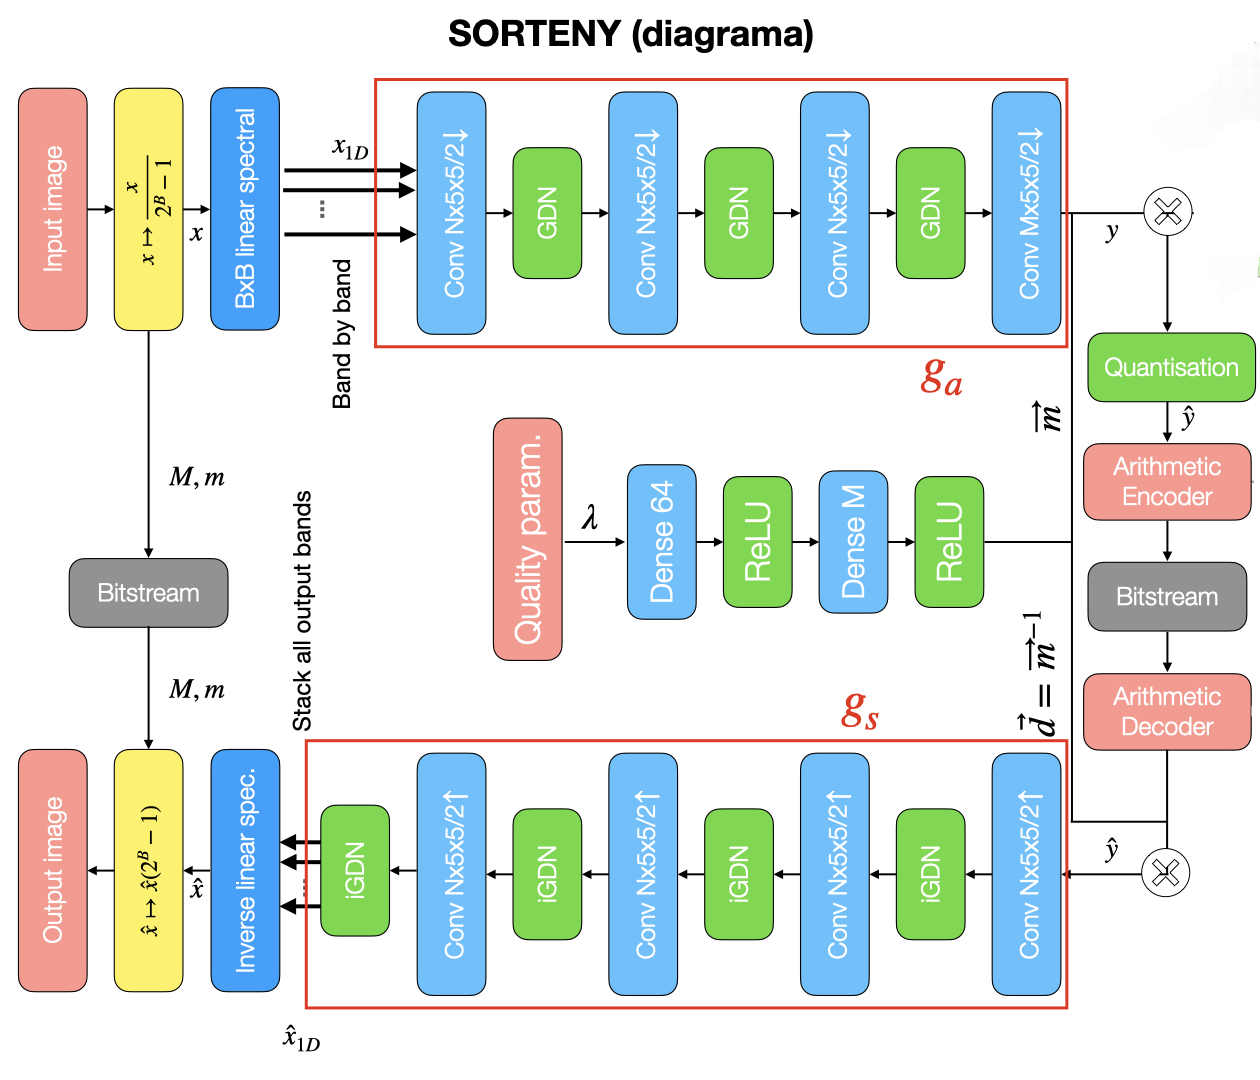
\includegraphics[width=0.94\textwidth]{ch2/sorteny_architecture.png}
\caption{Arquitectura conceptual de SORTENY: transformada espectral, transformada espacial, modulació de qualitat, quantització i síntesi.}
\label{fig:sorteny_architecture}
\figsource{Adaptat del treball previ propi \cite{anez2026treball}.}
\end{figure}

La transformada espectral redueix la redundància entre bandes projectant cada
píxel multiespectral a un espai de característiques après. Després, la
transformada espacial utilitza convolucions amb \emph{stride} i normalitzacions
GDN per compactar la informació en un tensor latent més petit. Finalment, una
subxarxa de modulació rep el paràmetre $\lambda$ i genera factors que escalen
els latents abans de la quantització. Un $\lambda$ més alt conserva més
informació i sol requerir més bits; un $\lambda$ més baix força més valors cap
a zero i augmenta la compressió.

Aquesta modulació és la propietat clau per a aquesta memòria. Si el model pot
canviar de qualitat amb un paràmetre, llavors es pot assignar un paràmetre de
qualitat diferent a cada regió de la imatge. El treball fixed-quality de
Mijares i Verdú \etal\ estudia justament com estimar el paràmetre necessari per
assolir un MSE objectiu local \cite{mijares2024fixed}. Aquesta base científica
permet passar d'una compressió uniforme a una compressió amb control espacial
de qualitat.

\section{Qualitat fixa, taxa fixa i regions d'interès}\label{sec:fixed_quality_art}

En compressió és important distingir taxa fixa i qualitat fixa. En un sistema
de taxa fixa, l'usuari imposa el volum màxim de dades; per exemple, ``aquesta
imatge ha d'ocupar com a màxim 2 MB''. El còdec intenta adaptar-se a aquest
límit i la qualitat final és la conseqüència. En un sistema de qualitat fixa,
l'usuari imposa una distorsió objectiu; per exemple, ``aquesta regió ha de
mantenir un PSNR mínim''. En aquest cas, la mida final del fitxer és la
conseqüència.

La qualitat fixa és atractiva en observació de la Terra perquè la utilitat de
la imatge no depèn només de la mida del fitxer, sinó de si les zones
científicament rellevants conserven prou informació. A diferència del
near-lossless, que sol limitar l'error màxim per mostra, el fixed-quality pot
formular objectius de MSE o PSNR sobre blocs o regions
\cite{mijares2024fixed}.

La regió d'interès (ROI) introdueix una pregunta addicional: no només cal
decidir quanta qualitat es vol, sinó on s'ha de preservar. Una imatge pot tenir
bon PSNR global i, alhora, degradar just la zona que l'usuari vol analitzar.
Els mètodes \emph{content-weighted} ja han explorat assignacions espacials de
qualitat en còdecs apresos \cite{li2018content}. En una plataforma embarcada,
però, la decisió espacial ha de ser barata, transparent i verificable.

Els índexs espectrals ofereixen una via simple per definir presets automàtics.
La forma habitual és comparar dues bandes amb un quocient normalitzat:

\begin{equation}
I(A,B)=\frac{A-B}{A+B}.
\label{eq:spectral_index_intro}
\end{equation}

Aquesta normalització redueix l'efecte de l'escala radiomètrica i permet
interpretar contrastos físics de manera aproximada. L'exemple més conegut és
l'NDVI:

\begin{equation}
\mathrm{NDVI}=\frac{\mathrm{NIR}-\mathrm{Red}}
{\mathrm{NIR}+\mathrm{Red}},
\end{equation}

on NIR és l'infraroig proper. Valors positius elevats solen indicar vegetació
activa, perquè la vegetació reflecteix fortament al NIR i absorbeix més al
vermell. Valors propers a zero poden correspondre a sòl nu o cobertes urbanes,
i valors negatius sovint apareixen en aigua, ombres o superfícies amb baixa
resposta NIR. Aquesta lectura és útil, però no és una classificació universal
\cite{rouse1974ndvi}.

Altres índexs segueixen la mateixa filosofia. L'NDWI contrasta verd i infraroig
proper per delinear aigua \cite{mcfeeters1996ndwi}; el GNDVI substitueix el
vermell pel verd per obtenir una variant sensible a vegetació
\cite{gitelson1996gndvi}; i l'NDCI es va proposar per estimar clorofil·la en
aigües productives \cite{mishra2012ndci}. El llindar depèn del sensor, de
l'atmosfera, de la reflectància, de la resolució i de l'escena. Per això
aquesta memòria parla de \emph{presets operatius}: regles interpretables que
seleccionen blocs candidats a rebre més qualitat, no etiquetes físiques
perfectes.

\section{Processament a bord i hardware de baix recurs}\label{sec:onboard_art}

La compressió a bord es justifica perquè l'enllaç de baixada, la memòria i el
temps disponible en un satèl·lit són limitats \cite{selva2012cubesats,
nasa2017cubesat}. Les missions petites i els CubeSats han impulsat l'ús de
components comercials i processadors de baix consum, però també introdueixen
restriccions de potència, temperatura, radiació i verificació
\cite{denis2017disruptions}.

La Raspberry Pi 3B+ utilitzada en aquesta memòria integra quatre nuclis
Cortex-A53 i 1~GB de memòria \cite{raspberry2018brief}. No és hardware
qualificat per a vol i pot patir problemes que no apareixen igual en un
ordinador terrestre, com alimentació insuficient, temperatura o susceptibilitat
a radiació \cite{guertin2021raspberry}. Tot i això, el Cortex-A53 i components
COTS han estat estudiats per a processament espacial \cite{schwaller2017a53},
i el C3SatP embarcat a Menut mostra una arquitectura COTS propera a aquest
rang de recursos \cite{serra2024c3satp}. Per tant, la Raspberry no certifica
vol, però sí és una plataforma raonable per mesurar ordres de magnitud de
temps, memòria i comportament tèrmic.

La implementació d'aquest treball utilitza C i OpenMP. OpenMP permet expressar
paral·lelisme de memòria compartida, però exigeix verificar que no s'introdueixen
carreres ni canvis d'ordre aritmètic \cite{openmp2021}. Per això les
optimitzacions posteriors es validen contra una baseline C abans d'acceptar-les.

Des del punt de vista d'assegurament del producte, aquesta memòria no
desenvolupa software de vol certificat. Les normes ECSS-E-ST-40C i
ECSS-Q-ST-80C indiquen què caldria per a un procés espacial complet:
requisits traçables, control de configuració, validació, verificació, gestió de
fallades i assegurament del producte software \cite{ecss40,ecss80}. Aquí es
cobreixen traçabilitat experimental, tests, manifests i reproducció, però no
qualificació de components, tolerància a fallades ni certificació.

\section{Síntesi del buit tecnològic}\label{sec:gap}

Aquest capítol mostra que les peces existeixen, però normalment apareixen
separades. CCSDS aporta estàndards madurs i eficients; els còdecs neuronals
aporten transformades apreses; el fixed-quality aporta control de distorsió;
els índexs espectrals aporten regles simples per seleccionar zones; i els
treballs d'execució a bord mostren la necessitat de controlar memòria i temps.

El buit que aborda aquesta memòria és la integració: convertir una transformada
apresa multiespectral en una ruta operativa que decideixi automàticament quines
zones protegir, assigni qualitat local, s'executi en C sense TensorFlow durant
l'operació i permeti mesurar tant la taxa codificada com el cost computacional
en hardware limitat.

La novetat del treball no és proposar un nou índex espectral ni un nou
autoencoder. La contribució és construir i validar una arquitectura que uneix
control espacial de qualitat, implementació C, presets automàtics, mesura de
bitrate codificat i avaluació en una plataforma de baix recurs. Els capítols
següents defineixen els fonaments tècnics necessaris i després descriuen la
implementació i els experiments.

\thispagestyle{empty}

\cleardoublepage
% !TEX root = ../main.tex
\chapter{Fonaments tècnics}\label{ch:fonaments}
\fancyhead[RE]{\slshape \textsf{Capítol \thechapter.\ Fonaments tècnics}}
\fancyhead[LO]{\slshape \textsf{\nouppercase \rightmark}}

\section{Dades multiespectrals i rang numèric}\label{sec:dades_multi}

Una adquisició multiespectral conté diverses mesures de la mateixa superfície
en intervals de longitud d'ona diferents. A Sentinel-2, per exemple, les bandes
B02, B03, B04 i B08 corresponen aproximadament al blau, verd, vermell i
infraroig proper; altres bandes cobreixen el red edge, vapor d'aigua o SWIR
\cite{esa2015sentinel2}. El producte original no té totes les bandes a la
mateixa resolució espacial. El conjunt de dades utilitzat en aquesta memòria
parteix de retalls ja preparats amb vuit bandes i una graella comuna de
$512\times512$ mostres.

La representació d'entrada és:

\begin{equation}
\mathbf{x}\in\{0,\ldots,65535\}^{B\times H\times W},
\qquad B=8,\;H=W=512.
\label{eq:input_tensor}
\end{equation}

El límit superior $65535$ no és arbitrari: és $2^{16}-1$, el valor màxim d'un
enter sense signe de 16 bits. Els fitxers RAW d'entrada s'emmagatzemen en aquest
format \code{uint16}. Abans d'entrar a la xarxa, les mostres es normalitzen a
l'interval aproximat $[0,1]$ dividint per aquest mateix valor, tal com es va
corregir i validar en la implementació C del treball previ
\cite{anez2026treball}.

La mida crua d'un retall és:

\begin{equation}
S_{\mathrm{raw}}=BHW\cdot2
=8\cdot512\cdot512\cdot2
=4\,194\,304\;\mathrm{bytes}.
\label{eq:raw_size}
\end{equation}

En aquesta memòria, quan s'utilitza \emph{bps}, es mesuren bits per mostra
espectral, és a dir, el denominador és $BHW$. Això és important perquè una
imatge multiespectral no conté només píxels espacials: conté píxels per banda.

La compressió és possible perquè hi ha redundància. La correlació espacial
permet predir una mostra a partir de les veïnes. La correlació espectral permet
expressar una banda a partir de combinacions d'altres bandes. SORTENY tracta
aquestes dues fonts de redundància amb transformades apreses.

\section{SORTENY des del punt de vista de la implementació}
\label{sec:arquitectura}

Després de situar SORTENY en el context dels còdecs neuronals per a observació
de la Terra, cal concretar quins elements interns fan possible el control de
qualitat que s'estudia en aquesta memòria. En particular, aquest capítol
descriu la geometria de la xarxa, les operacions amb més cost computacional, el
paper del modulador de qualitat i les mètriques que s'utilitzaran per avaluar
els resultats.

El pipeline conceptual és:

\begin{equation}
\mathbf{x}\xrightarrow{g_a}
\mathbf{y}\xrightarrow{\mathcal{Q}_{\lambda}}
\hat{\mathbf{y}}\xrightarrow{g_s}\hat{\mathbf{x}}.
\label{eq:sorteny_pipeline}
\end{equation}

$g_a$ és la transformada d'anàlisi, $\mathbf{y}$ són els latents,
$\mathcal{Q}_{\lambda}$ és la quantització condicionada pel paràmetre de
qualitat i $g_s$ és la transformada de síntesi. Els pesos ja estan entrenats.
El treball d'aquesta memòria es centra en executar i controlar aquesta
inferència, no en reentrenar la xarxa.

\subsection{Transformada espectral}

La transformada espectral combina les $B$ bandes en cada posició espacial. En
forma simplificada:

\begin{equation}
\mathbf{z}_{h,w}=\mathbf{W}_{s}\mathbf{x}_{h,w}.
\label{eq:spectral_transform}
\end{equation}

$\mathbf{W}_{s}$ és una matriu apresa. A diferència d'una transformada fixa,
pot adaptar-se a l'estadística del conjunt d'entrenament. Computacionalment,
l'operació és independent entre posicions espacials: cada píxel pot processar-se
separadament, mantenint l'ordre intern de suma sobre bandes. Aquesta propietat
és rellevant quan es paral·lelitza el C sense alterar el resultat numèric.

\subsection{Convolucions i cost principal}

Les convolucions redueixen progressivament la resolució espacial i concentren
informació en canals latents. Una convolució amb kernel $K\times K$ pot
escriure's com:

\begin{equation}
y_{c_o,h,w}=b_{c_o}+
\sum_{c_i}\sum_{u=0}^{K-1}\sum_{v=0}^{K-1}
W_{c_o,c_i,u,v}\,x_{c_i,h+u,w+v}.
\label{eq:conv2d}
\end{equation}

La fórmula mostra per què és una operació costosa. Per cada mostra de sortida
cal recórrer canals d'entrada i posicions del kernel. En SORTENY, els kernels
espacials són de $5\times5$ i el nombre de canals intermedis és elevat. Per
això, el temps total del còdec està dominat per aquestes operacions i no pel
càlcul de regles semàntiques senzilles com un índex espectral.

\subsection{GDN i IGDN}

Entre convolucions s'utilitza \emph{Generalized Divisive Normalization} (GDN),
una normalització no lineal habitual en compressió neuronal
\cite{balle2017end}. Per una posició espacial fixa:

\begin{equation}
y_i=\frac{x_i}
{\sqrt{\beta_i+\sum_j\gamma_{ij}x_j^2}}.
\label{eq:gdn}
\end{equation}

El canal $i$ no depèn només d'ell mateix, sinó també de la suma ponderada dels
altres canals $j$. La IGDN aplica la transformació complementària al decoder.
A diferència d'una activació simple com ReLU, la GDN no només talla o escala
valors de manera independent: normalitza cada resposta segons l'energia dels
altres canals. En compressió neuronal això és útil perquè tendeix a reduir
dependències estadístiques entre coeficients latents, un efecte sovint descrit
com una aproximació a ``gaussianitzar'' o fer més regular la distribució dels
coeficients. Uns latents menys dependents són més adequats per al model de
probabilitat i per al codificador per entropia posterior.

Aquest guany de modelatge té un cost computacional: cal calcular sumes entre
canals per moltes posicions espacials. Aquesta és una de les raons per les quals
l'optimització C ha de respectar l'ordre de les operacions i validar paritat
numèrica.

\subsection{Modulador de qualitat}

SORTENY és multiràtio perquè incorpora una subxarxa de modulació condicionada
pel paràmetre $\lambda$ \cite{mijares2023reduced,mijares2025sorteny}. El
modulador genera factors que escalen els latents abans de quantitzar-los i que
el decoder necessita per invertir l'operació de manera coherent.

És important no confondre $M(\lambda)$ amb una màscara ROI. $M(\lambda)$ és un
tensor de factors de modulació après, amb la mateixa funció conceptual per a
tota la imatge o per cada posició latent. Una màscara ROI, en canvi, és una
decisió externa sobre quines zones es volen prioritzar. El Q-map que es defineix
més endavant tradueix aquesta decisió externa a valors de $\lambda$ quantitzats,
però el modulador continua sent el mecanisme intern de la xarxa.

\section{Geometria interna i granularitat del Q-map}
\label{sec:tensor_geometry}

La geometria dels tensors explica dues propietats centrals: el cost de memòria
i la mida de la graella de control de qualitat. La transformada espectral opera
a resolució completa. Després, cada component passa per quatre convolucions de
stride 2. Cada stride 2 redueix l'alçada i l'amplada a la meitat:

\begin{figure}[H]
\centering
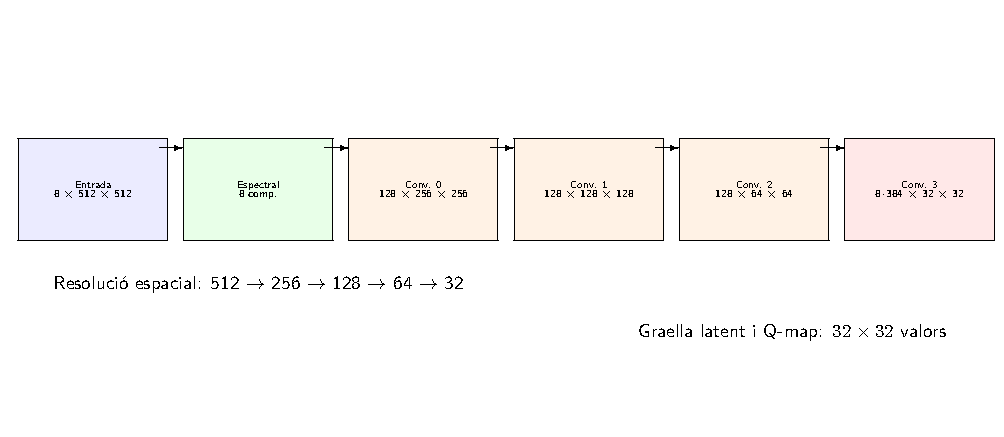
\includegraphics[width=0.92\textwidth]{ch3/tensor_geometry_funnel.pdf}
\caption{Reducció espacial de SORTENY fins a la graella latent. La figura
mostra dimensions conceptuals; la implementació reutilitza buffers i no conserva
tots els tensors simultàniament.}
\label{fig:tensor_geometry_funnel}
\end{figure}

\begin{table}[H]
\centering
\small
\begin{tabular}{lrrrrl}
\toprule
Etapa & Canals & Alçada & Amplada & Valors & Operació posterior \\
\midrule
Entrada per banda & 1 & 512 & 512 & 262.144 & Conv. 0 \\
Anàlisi 0 & 128 & 256 & 256 & 8.388.608 & GDN \\
Anàlisi 1 & 128 & 128 & 128 & 2.097.152 & GDN \\
Anàlisi 2 & 128 & 64 & 64 & 524.288 & GDN \\
Latent per component & 384 & 32 & 32 & 393.216 & Modulació i Q \\
Latent complet & $8\cdot384$ & 32 & 32 & 3.145.728 & Codificació \\
\bottomrule
\end{tabular}
\caption{Dimensions principals derivades dels pesos i de la implementació C.
La columna \emph{Valors} indica el nombre d'elements del tensor, no la memòria
total reservada durant tota la inferència.}
\label{tab:tensor_geometry}
\end{table}

El màxim tensor intermedi d'una banda conté més de vuit milions de
\code{float32}, uns 32~MiB. Conservar còpies independents per capa o per fil
superaria ràpidament la memòria disponible en una plataforma de baix recurs.
Aquesta geometria justifica la reutilització de buffers que s'explica al
Capítol~\ref{ch:pipeline}.

\subsection{\texorpdfstring{De $512\times512$ a $32\times32$}{De 512x512 a 32x32}}

Quatre reduccions per factor 2 donen un factor total $2^4=16$. Per tant:

\begin{equation}
\frac{512}{16}=32.
\label{eq:qmap_grid_size}
\end{equation}

El control espacial de qualitat opera sobre aquesta graella latent de
$32\times32$ posicions. De manera pràctica, es parla d'un valor Q per bloc
$16\times16$ de la imatge d'entrada. Aquesta frase descriu la graella de
control, però no vol dir que cada bloc sigui independent visualment.

\begin{figure}[H]
\centering
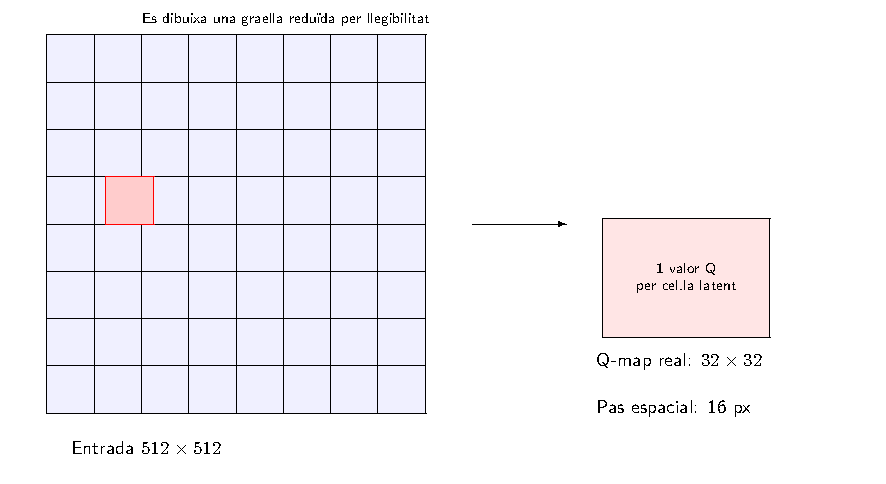
\includegraphics[width=0.82\textwidth]{ch3/qmap_grid.pdf}
\caption{Correspondència entre la imatge d'entrada i el Q-map. Cada valor Q
controla una cel·la latent associada a un pas de 16 píxels a l'entrada.}
\label{fig:qmap_grid}
\end{figure}

\subsection{Camp receptiu i efecte sobre ROIs petites}

Una cel·la latent no depèn només dels $16\times16$ píxels que li corresponen
per pas espacial. Les convolucions amb kernel $5\times5$ fan que cada sortida
vegi un veïnat de l'entrada. Si $r_\ell$ és la mida del camp receptiu després
de la capa $\ell$ i $j_\ell$ és el salt equivalent entre posicions d'aquella
capa respecte l'entrada:

\begin{equation}
r_0=1,\qquad j_0=1,
\end{equation}

\begin{equation}
r_{\ell+1}=r_\ell+(5-1)j_\ell,\qquad
j_{\ell+1}=2j_\ell.
\label{eq:receptive_field}
\end{equation}

Això dona:

\begin{table}[H]
\centering
\small
\begin{tabular}{lrrrrr}
\toprule
Després de la capa & 0 & 1 & 2 & 3 & 4 \\
\midrule
Salt equivalent $j$ & 1 & 2 & 4 & 8 & 16 \\
Camp receptiu $r$ & 1 & 5 & 13 & 29 & 61 \\
\bottomrule
\end{tabular}
\caption{Creixement del camp receptiu amb quatre convolucions $5\times5$ i
stride 2.}
\label{tab:receptive_field}
\end{table}

La conseqüència és important per a la qualitat espacial: una ROI petita o molt
dispersa pot quedar afectada pels blocs veïns. Encara que la cel·la latent
marcada com a ROI rebi una qualitat alta, part de la informació que contribueix
a reconstruir-la pot haver passat per cel·les properes amb una qualitat diferent.

\begin{figure}[H]
\centering
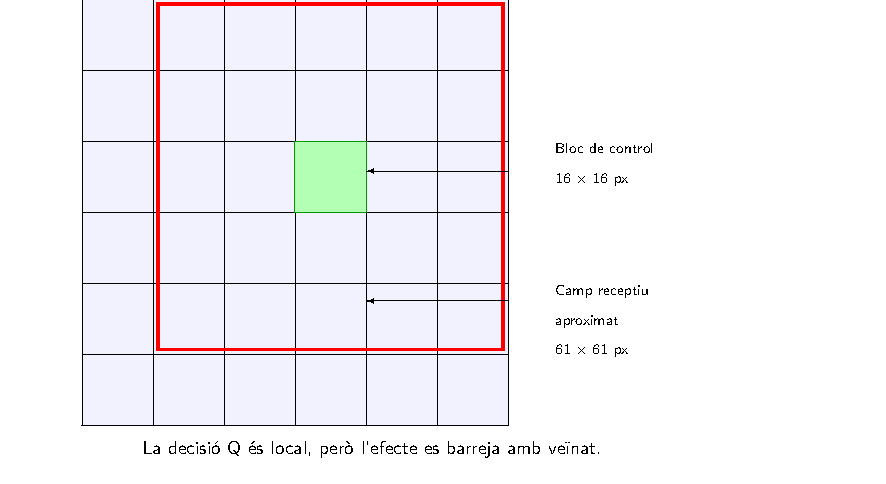
\includegraphics[width=0.78\textwidth]{ch3/receptive_field_overlap.pdf}
\caption{Diferència entre graella de control i camp d'influència. El bloc de
control és de 16 píxels, però el camp receptiu teòric arriba aproximadament a
61 píxels.}
\label{fig:receptive_field_overlap}
\end{figure}

\section{Taxa, distorsió i qualitat}\label{sec:metriques_teoria}

\subsection{MSE, MAE i PSNR}

Per a $N=BHW$ mostres, l'error quadràtic mitjà és:

\begin{equation}
\mathrm{MSE}(\mathbf{x},\hat{\mathbf{x}})
=\frac{1}{N}\sum_{i=1}^{N}(x_i-\hat{x}_i)^2.
\label{eq:mse}
\end{equation}

L'error absolut mitjà és:

\begin{equation}
\mathrm{MAE}(\mathbf{x},\hat{\mathbf{x}})
=\frac{1}{N}\sum_{i=1}^{N}|x_i-\hat{x}_i|.
\label{eq:mae}
\end{equation}

Per dades de 16 bits, el PSNR es calcula amb el mateix màxim dinàmic que a
l'Equació~\ref{eq:input_tensor}:

\begin{equation}
\mathrm{PSNR}=10\log_{10}
\left(\frac{65535^2}{\mathrm{MSE}}\right)\;\mathrm{dB}.
\label{eq:psnr}
\end{equation}

Un PSNR més alt implica menys MSE. La diferència en dB és logarítmica; no es
pot interpretar linealment com un percentatge de píxels correctes. El PSNR és
especialment adequat en aquest treball perquè el model fixed-quality que
s'utilitza com a base científica està formulat en termes de MSE
\cite{mijares2024fixed}. Altres mètriques, com SSIM, modelen estructura visual
\cite{wang2004ssim}, però no són la variable que calibra el mètode.

\subsection{Bitrate i fitxer \code{.tfci}}

El bitrate es mesura en bits per mostra espectral:

\begin{equation}
R=\frac{8S}{BHW}\;\bps,
\label{eq:bps_general}
\end{equation}

on $S$ és la mida codificada en bytes. Quan el fitxer és el resultat del
pipeline de TensorFlow Compression, s'utilitza l'extensió \code{.tfci}. Aquest
fitxer conté latents codificats i la informació lateral que el decoder de la
referència necessita per reconstruir la imatge. Per això és la mesura que
s'utilitza com a bitrate real en les validacions CSMR.

\begin{equation}
R_{\mathrm{tfci}}=
\frac{8S_{\mathrm{tfci}}}{BHW}\;\bps.
\label{eq:bps}
\end{equation}

El bitstream C d'aquesta memòria té una funció diferent: empaqueta capçalera,
Q-map i latents per validar la ruta C, però encara no incorpora el mateix
codificador per entropia o codificador aritmètic que la referència. Per aquest
motiu, la mida C directa no s'interpreta com a bitrate final de compressió.

Si un mètode A té bitrate $R_A$ i el baseline B té $R_B$, l'estalvi relatiu és:

\begin{equation}
\mathrm{estalvi}_{A/B}
=100\left(1-\frac{R_A}{R_B}\right)\%.
\label{eq:saving}
\end{equation}

Un estalvi del 10\% significa que A envia el 90\% dels bits de B. No equival a
dir que la compressió s'ha duplicat.

\subsection{Entropia i proxies}

L'entropia empírica d'un alfabet latent és:

\begin{equation}
H=-\sum_k p_k\log_2 p_k.
\label{eq:entropy}
\end{equation}

Una entropia menor suggereix que els símbols podrien codificar-se amb menys
bits, però no especifica el resultat d'un codificador concret
\cite{cover2006information}. També es pot aplicar una compressió generalista
com zlib per obtenir un indici ràpid de compresibilitat. En aquesta memòria,
entropia i zlib són proxies de selecció: ajuden a decidir quins casos mereixen
una validació completa, però no substitueixen el bitrate \code{.tfci}.

\section{Qualitat espacial, ROI i fons}\label{sec:roi_metrics}

Una regió d'interès, o ROI, és el conjunt de blocs que es vol protegir amb més
qualitat. En aquest capítol la definició és deliberadament genèrica: la màscara
pot venir d'un operador manual, d'un criteri espectral o d'un altre mecanisme.
Els capítols següents definiran els mecanismes concrets utilitzats.

Sigui $m_{u,v}\in\{0,1\}$ la màscara sobre la graella latent
$32\times32$. Els blocs amb $m=1$ formen la ROI i els blocs amb $m=0$ formen el
fons. Per mesurar PSNR sobre la imatge d'entrada, aquesta màscara de blocs
s'expandeix a les mostres espacials corresponents.

Per una reconstrucció A i un baseline B, sempre amb la mateixa màscara:

\begin{align}
\Delta\mathrm{PSNR}_{\mathrm{ROI}}
&=\mathrm{PSNR}_{\mathrm{ROI}}(A)
-\mathrm{PSNR}_{\mathrm{ROI}}(B),\\
\Delta\mathrm{PSNR}_{\mathrm{fons}}
&=\mathrm{PSNR}_{\mathrm{fons}}(A)
-\mathrm{PSNR}_{\mathrm{fons}}(B).
\label{eq:roi_bg_deltas}
\end{align}

Usar la mateixa màscara és essencial. Si el baseline i el mètode avaluat es
mesuressin sobre regions diferents, els deltes no compararien la mateixa
població de mostres. Una política espacial útil ha de conservar o millorar la
ROI respecte del baseline escollit, mentre pot degradar el fons de manera
controlada si això redueix el bitrate.

La cobertura de la ROI és:

\begin{equation}
C_{\mathrm{ROI}}=
\frac{\sum_{u,v}m_{u,v}}{32\cdot32}\cdot100\%.
\label{eq:roi_coverage}
\end{equation}

Els extrems són poc informatius. Si $C_{\mathrm{ROI}}=0$, no hi ha cap regió
protegida. Si $C_{\mathrm{ROI}}=100\%$, tota la imatge és ROI i no queda fons
d'on obtenir estalvi. Entre aquests extrems, la mida i la forma de la ROI
condicionen la utilitat del control espacial.

\section{Model fixed-quality}\label{sec:model_fq}

El mètode fixed-quality de Mijares i Verdú \etal\ parteix d'una pregunta
inversa: en lloc de provar diferents qualitats fins trobar-ne una adequada,
estima quin $\lambda$ cal utilitzar per assolir un error objectiu
\cite{mijares2024fixed}.

\subsection{De PSNR objectiu a MSE objectiu}

Si l'usuari defineix una qualitat objectiu en PSNR, primer cal convertir-la a
MSE. Reordenant l'Equació~\ref{eq:psnr}:

\begin{equation}
\widehat{\mathrm{MSE}}=
\frac{65535^2}
{10^{\mathrm{PSNR}_{\mathrm{obj}}/10}}.
\label{eq:target_mse}
\end{equation}

El símbol $\widehat{\mathrm{MSE}}$ indica l'error que es voldria obtenir. Aquest
valor no determina directament el byte d'un Q-map. Abans cal tenir en compte
l'error base de la imatge o del bloc.

\subsection{MSE base i modulador mitjà}

El paper defineix $\mathrm{MSE}_0(\mathbf{x})$ com l'error base o mínim associat
a la imatge $\mathbf{x}$ en el model considerat. Aquest valor depèn del
contingut: dues imatges comprimides amb el mateix $\lambda$ poden donar PSNR
diferents perquè no tenen la mateixa dificultat de reconstrucció.

La magnitud mitjana del modulador es modela com una funció lineal:

\begin{equation}
\bar{M}(\lambda)=a\lambda+b.
\label{eq:mod_linear}
\end{equation}

El paper observa que l'error de reconstrucció creix de manera aproximadament
quadràtica amb l'invers d'aquest modulador mitjà. La relació s'escriu com:

\begin{equation}
\widehat{\mathrm{MSE}}
=\mathrm{MSE}_0+
\alpha\,\mathrm{MSE}_0
\left(\frac{1}{2\bar{M}(\lambda)}\right)^2.
\label{eq:mse_model}
\end{equation}

Dividint per $\mathrm{MSE}_0$, es veu millor la idea de l'error relatiu:

\begin{equation}
\frac{\widehat{\mathrm{MSE}}}{\mathrm{MSE}_0}
=1+
\alpha
\left(\frac{1}{2\bar{M}(\lambda)}\right)^2.
\label{eq:mse_relative_model}
\end{equation}

Aquesta expressió és una aproximació estadística calibrada. No diu que tots els
píxels tinguin el mateix error, sinó que permet estimar quin $\lambda$ produeix
un error mitjà esperat.

\subsection{Estimació de \texorpdfstring{$\lambda$}{lambda}}

Combinant les Equacions~\ref{eq:mod_linear} i~\ref{eq:mse_model}, el paper
despeja el valor de $\lambda$ necessari:

\begin{equation}
\hat{\lambda}
=\frac{1}{a}
\left(
\sqrt{
\frac{\alpha\,\mathrm{MSE}_0(\mathbf{x})}
{4\left(\widehat{\mathrm{MSE}}-\mathrm{MSE}_0(\mathbf{x})\right)}
}
-b
\right).
\label{eq:lambda_from_mse}
\end{equation}

La cadena completa és, per tant:

\begin{figure}[H]
\centering
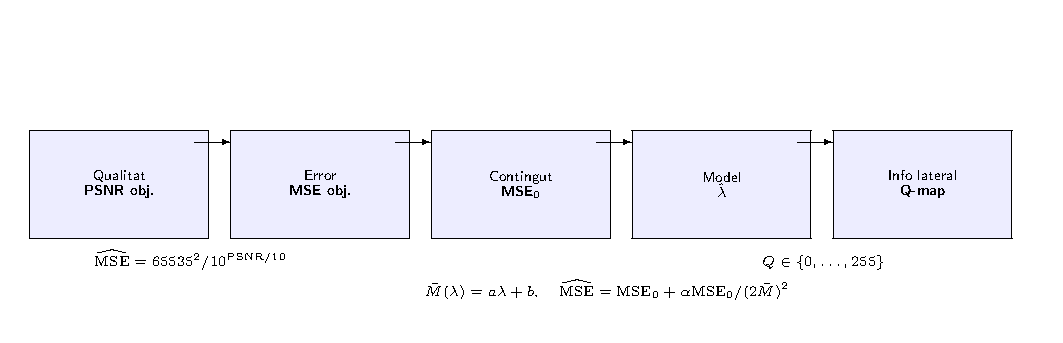
\includegraphics[width=0.92\textwidth]{ch3/fixed_quality_chain.pdf}
\caption{Cadena conceptual del model fixed-quality: d'una qualitat objectiu es
dedueix un MSE objectiu, després un $\lambda$ estimat i finalment una
representació quantitzada per transmetre al decoder.}
\label{fig:fixed_quality_chain}
\end{figure}

L'Equació~\ref{eq:lambda_from_mse} només té sentit si el target és assolible:
el denominador ha de ser positiu i el resultat ha de quedar dins el rang de
$\lambda$ per al qual el model i la calibració són vàlids. Quan no passa, el
sistema ha de saturar al límit disponible o marcar el cas com no assolible.

\subsection{Quantització de \texorpdfstring{$\lambda$}{lambda} a Q}

Un array de $\lambda$ en coma flotant seria informació lateral costosa. El paper
quantitza cada $\lambda$ a un enter de 8 bits:

\begin{equation}
Q=
\operatorname{round}\left[
255\frac{\lambda-\lambda_{\min}}
{\lambda_{\max}-\lambda_{\min}}
\right],
\qquad Q\in\{0,\ldots,255\}.
\label{eq:lambda_to_q}
\end{equation}

El decoder pot recuperar el valor aproximat amb:

\begin{equation}
\hat{\lambda}=
\lambda_{\min}+
\frac{Q}{255}
(\lambda_{\max}-\lambda_{\min}).
\label{eq:q_to_lambda}
\end{equation}

Per tant, el byte Q no és una quantització clàssica directa dels píxels. És una
quantització lineal del paràmetre $\lambda$, que després actua a través del
modulador de la xarxa. En aquesta arquitectura, valors Q més alts corresponen a
valors $\lambda$ més alts i, en general, a més qualitat i més taxa.

\subsection{Cost de la informació lateral}

Quan la qualitat varia espacialment, el decoder ha de conèixer quina qualitat
s'ha aplicat a cada posició latent. Aquesta informació no forma part de la
imatge reconstruïda, però és necessària per poder descodificar-la correctament;
per això s'anomena \emph{informació lateral}. En la ruta C d'aquesta memòria,
aquesta informació lateral és el Q-map escrit explícitament al bitstream
intermedi.

Amb una graella $32\times32$, un Q-map conté 1.024 valors. Si cada valor és un
byte, la informació lateral ocupa 1.024 bytes. Expressada en bits per píxel
espacial, la mateixa convenció que utilitza el paper fixed-quality per comparar
arrays de $\lambda$, aquesta mida és:

\begin{equation}
R_{Q,\mathrm{espacial}}=
\frac{8\cdot1024}{512\cdot512}
=0.03125\;\text{bits/píxel}.
\label{eq:qmap_side_spatial_bps}
\end{equation}

La resta de resultats d'aquesta memòria, però, es donen en bits per mostra
espectral. Com que cada retall té vuit bandes, el mateix cost es reparteix sobre
$8\cdot512\cdot512$ mostres:

\begin{equation}
R_Q=
\frac{8\cdot1024}{8\cdot512\cdot512}
=0.00390625\;\bps.
\label{eq:qmap_side_bps}
\end{equation}

La diferència entre $0.03125$ i $0.00390625$ no és una contradicció; només
canvia el denominador. La informació lateral és petita respecte del volum RAW,
però és real i s'ha de transportar o reconstruir de manera equivalent al
decoder.

\section{Lectura dels capítols següents}\label{sec:criteris_lectura}

Amb aquests fonaments es pot separar el problema en tres decisions. Primer,
quin valor de qualitat es vol assignar. Segon, si aquest valor és global o pot
variar sobre la graella $32\times32$. Tercer, quin criteri decideix quins blocs
mereixen més o menys qualitat.

Els capítols següents concreten aquestes decisions en una implementació C i en
experiments. El Capítol~\ref{ch:pipeline} descriu el còdec i el bitstream. El
Capítol~\ref{ch:control} defineix els modes de Q-map i els presets automàtics.
El Capítol~\ref{ch:metodologia} explica com es mesuren resultats amb màscares
comunes, C-only i CSMR. Finalment, els capítols de resultats indiquen quins
compromisos taxa--distorsió s'obtenen i quin cost tenen en una plataforma de
baix recurs.

\thispagestyle{empty}

\cleardoublepage
% !TEX root = ../main.tex
\chapter{Treball previ i evolució del pipeline C}\label{ch:pipeline}
\fancyhead[RE]{\slshape \textsf{Capítol \thechapter.\ Pipeline C}}
\fancyhead[LO]{\slshape \textsf{\nouppercase \rightmark}}

\section{Antecedent propi}\label{sec:antecedent}

El punt de partida d'aquesta memòria és un treball propi anterior sobre la
portabilitat de SORTENY a C \cite{anez2026treball}. Aquell treball ja havia
demostrat que una part substancial del compressor neuronal podia executar-se
sense el runtime de TensorFlow: es van exportar pesos, es van implementar
operadors de la transformada d'anàlisi i es va reduir el consum de memòria amb
buffers reutilitzables.

En una imatge de prova, el compressor C anterior va passar d'uns 796,5~MiB de
la ruta Python a uns 87~MiB, i va obtenir una acceleració aproximada
d'$1,47\times$. La comparació dels latents va mostrar un 99,9876\% de valors
idèntics, amb discrepàncies de $\pm1$ en una fracció petita. Aquest resultat
era suficient per validar la direcció, però encara no constituïa un còdec
complet: faltava una ruta de descompressió, un mecanisme de qualitat espacial,
una validació de bitstream i una mesura de bitrate codificat.

\subsection{Què s'hereta i què s'afegeix}

La Taula~\ref{tab:herencia} separa el treball heretat de les aportacions
d'aquesta memòria. La lectura important és que no es torna a entrenar SORTENY:
es construeix una ruta C al voltant del model entrenat i se'n completa el cicle
compressió--descompressió.

\begin{table}[H]
\centering
\scriptsize
\begin{tabularx}{\textwidth}{p{2.9cm}X X X}
\toprule
Component & Estat al treball previ & Aportació actual & Per què importa \\
\midrule
Pesos entrenats & Exportació inicial de pesos de l'encoder. & Validació de
formes, pesos d'encoder i decoder i índexs de càrrega. & Evita errors de
layout que poden donar sortides plausibles però incorrectes. \\
Compressor C & Transformada d'anàlisi funcional. & Integració amb informació
de qualitat local i contenidor autocontingut. & Permet transportar la qualitat
aplicada juntament amb els latents. \\
Descompressor & No era la ruta principal. & Implementació completa de síntesi,
validació de capçalera i reconstrucció RAW. & Tanca el còdec i permet verificar
que el fitxer generat és llegible. \\
Qualitat & Un únic paràmetre global. & Mapa local de qualitat i calibració
associada. & Fa possible protegir unes zones i degradar-ne unes altres. \\
Bitrate & Proxies sobre latents. & Mesura externa amb codificació real de la
referència. & Separa compressibilitat estimada de bitrate codificat. \\
Raspberry & Prova inicial de compressor. & Pipeline complet, optimització i
mesura de cost de qualitat local. & Aproxima el comportament en hardware de
baix recurs. \\
\bottomrule
\end{tabularx}
\caption{Separació entre l'antecedent propi i les aportacions d'aquesta
memòria.}
\label{tab:herencia}
\end{table}

\section{Referència Python i contracte funcional}\label{sec:python_ref}

SORTENY disposa d'una implementació Python de referència. En aquesta memòria
no es presenta com a producte operatiu, sinó com a definició executable del
model entrenat: conté la càrrega de checkpoints, les transformades, la
modulació de qualitat i el codificador final de TensorFlow Compression. Els
camins exactes del repositori i les ordres de reproducció es documenten als
apèndixs i al repositori públic associat; en el cos principal només interessa
la seva funció metodològica.

Portar aquesta referència a C no consisteix a traduir sintaxi. En Python, el
framework conserva molta informació de forma implícita: ordre de dimensions,
padding de convolucions, disposició dels kernels, tipus de dades, arrodoniment,
normalització i empaquetat final. En C, totes aquestes decisions han de quedar
fixades de manera explícita. Un error petit en un índex pot no provocar cap
fallada d'execució, però sí canviar els latents i, per tant, la reconstrucció.

La referència Python manté dues responsabilitats durant aquest treball:

\begin{itemize}[leftmargin=*]
  \item servir com a patró funcional del model entrenat;
  \item proporcionar una codificació final real, mitjançant fitxers
  \code{.tfci}, per mesurar bitrate quan el contenidor C encara no inclou un
  codificador per entropia o aritmètic equivalent.
\end{itemize}

\subsection{Frontera entre referència i ruta C}

La Taula~\ref{tab:python_c_contract} resumeix la frontera. El criteri és
pragmàtic: la ruta C ha d'executar el model i reconstruir la imatge amb recursos
limitats; la referència conserva les eines de model i de codificació final que
encara no s'han portat a C.

\begin{table}[H]
\centering
\small
\begin{tabularx}{\textwidth}{p{3.3cm}X X}
\toprule
Funció & Referència de model & Ruta C operativa \\
\midrule
Càrrega del model & Checkpoints i objectes TensorFlow. & Fitxers de pesos
binaris i índexs de formes. \\
Qualitat global & Valor continu del paràmetre de qualitat. & Valor global
equivalent quantitzat o transmès com a configuració. \\
Qualitat local & Array local acceptat per la referència. & Mapa local de
1.024 bytes transportat dins el contenidor C. \\
Transformades & Operadors del framework. & Bucles C, OpenMP i buffers
explícits. \\
Codificació final & TensorFlow Compression, fitxer \code{.tfci}. & Latents
enters dins un contenidor intermedi, sense codificació final eficient. \\
Ús al projecte & Patró funcional i bitrate real. & Ruta candidata per a
execució en hardware limitat. \\
\bottomrule
\end{tabularx}
\caption{Contracte entre la referència de model i la ruta C.}
\label{tab:python_c_contract}
\end{table}

La separació també condiciona la validació. Les diferències C--Python poden
venir de coma flotant, arrodoniment o detalls interns del framework. En canvi,
dues versions C comparades sota el mateix entorn han de produir la mateixa
reconstrucció si només s'ha optimitzat el codi. Per això la paritat C--C és el
criteri estricte quan es canvia la implementació C, mentre que la referència
Python actua com a comprovació externa del comportament del model.

\section{Implementació C del model}\label{sec:c_software_arch}

El model entrenat es considera congelat. La ruta C no aprèn pesos nous ni
modifica l'arquitectura; implementa la inferència, la lectura de pesos, la
informació de qualitat local i el contenidor necessari perquè el decoder pugui
reconstruir. Aquesta separació és important: les decisions científiques del
model provenen de SORTENY, mentre que aquesta memòria se centra en fer-lo
executables, verificable i mesurable en un entorn limitat.

\subsection{Mòduls i responsabilitats}\label{sec:pesos}

La implementació es divideix en responsabilitats conceptuals. Els noms exactes
de fitxer són traçables al repositori, però la Taula~\ref{tab:c_modules} mostra
la idea d'arquitectura.

\begin{table}[H]
\centering
\small
\begin{tabularx}{\textwidth}{p{3.0cm}X X}
\toprule
Mòdul conceptual & Responsabilitat & Validació associada \\
\midrule
Càrrega de model & Llegeix pesos, formes i índexs. & Mides esperades,
coherència de canals i presència de pesos mínims. \\
Operadors neuronals & Executa convolucions, GDN/IGDN, capes denses i
reordenacions. & Tests amb tensors petits i comparació amb valors esperats. \\
Entrada i sortida RAW & Llegeix BSQ \code{uint16}, controla endianess i escriu
la reconstrucció. & Mida exacta del RAW i rang $[0,65535]$. \\
Compressor & Aplica transformades, modulació i quantització. & Contenidor
estructuralment vàlid i latents coherents. \\
Descompressor & Valida el contenidor, desfà la modulació i sintetitza la
imatge. & Reconstrucció completa i verificació de dimensions. \\
Generadors de qualitat & Calculen el mapa local de qualitat a partir de
configuració o criteris automàtics. & Mapa de 1.024 bytes i traçabilitat de la
decisió. \\
\bottomrule
\end{tabularx}
\caption{Responsabilitats principals de la ruta C.}
\label{tab:c_modules}
\end{table}

Els pesos no es carreguen com una col·lecció opaca de fitxers. Cada tensor va
acompanyat d'un índex que indica nom, tipus, forma i mida. Aquesta informació
és fonamental perquè la xarxa combina moltes dimensions: canals d'entrada,
canals de sortida, kernels espacials, factors de modulació i transformades
espectrals. Si un kernel es llegís transposat, el programa podria acabar sense
errors però generaria una imatge incorrecta. Per això el carregador comprova la
mida esperada i la compatibilitat de canals abans d'associar cada buffer al
model.

\subsection{Punts crítics de la traducció a C}\label{sec:operadors}

Els operadors C reprodueixen la mecànica descrita al
Capítol~\ref{ch:fonaments}: convolucions amb stride, GDN i IGDN, capes denses
del modulador, reordenacions espacials i transformada espectral. El problema no
és escriure una fórmula a C, sinó conservar totes les convencions que el
framework gestiona de forma implícita.

Hi ha quatre punts especialment sensibles. Primer, les convolucions redueixen
resolució i canvien el nombre de canals; una transposició de kernel pot produir
una sortida amb la mida correcta però amb valors incorrectes. Segon, GDN i IGDN
fan sumes entre canals amb paràmetres apresos $\beta$ i $\gamma$; canviar
l'ordre o confondre canals altera la normalització. Tercer, el modulador de
qualitat genera factors que escalen els latents abans de l'arrodoniment; per
tant, un error de qualitat es propaga directament al fitxer. Quart, les
reordenacions del decoder no fan operacions de coma flotant, però són molt
sensibles a l'ordre de canals i píxels.

Aquests detalls expliquen per què els tests d'operadors no són un accessori:
un error de layout pot quedar poc visible en una imatge reconstruïda, però
trencar la paritat i fer que el decoder llegeixi una estructura diferent de la
que el compressor ha escrit.

La transformada espectral també té dues cares: anàlisi abans de la compressió
espacial i síntesi després del decoder. La ruta oficial utilitza pesos de
síntesi validats. El codi conserva una salvaguarda de compatibilitat per
derivar una inversa quan falten aquests pesos, però aquesta ruta no és la base
de cap resultat experimental de la memòria.

\subsection{Per què desacoblar qualitat i inferència}

Una decisió de disseny és separar la generació de qualitat local de la
inferència del model. Un bloc de codi decideix quina qualitat ha de tenir cada
cel·la de la graella; un altre bloc executa les transformades neuronals amb
aquesta informació. La frontera entre tots dos blocs és el mapa de qualitat:
una graella de 1.024 bytes que el compressor només consumeix, sense saber si
prové d'una qualitat global, d'una calibració o d'un criteri automàtic.

Aquesta separació redueix risc experimental. Afegir un criteri nou de selecció
de regions no modifica les convolucions ni els pesos; només canvia el mapa que
entra al compressor. Inversament, optimitzar GDN, IGDN o la transformada
espectral no altera la decisió de quina regió és prioritària. Així es poden
provar polítiques de qualitat i optimitzacions C per separat, amb validacions
diferents.

Aquest desacoblament és el pont cap al Capítol~\ref{ch:control}: aquí només es
descriu que el compressor accepta una qualitat global o local; el capítol
següent defineix formalment quins modes de qualitat s'han implementat.

\section{Gestió de memòria}\label{sec:memoria}

La memòria és una restricció central. Una implementació directa podria reservar
la sortida de cada capa per a totes les bandes i conservar-la fins al final.
Això és còmode en un framework de xarxa neuronal, però no és adequat per a una
placa de baix recurs. La ruta C tracta els tensors intermedis com a dades amb
vida curta: quan una capa ja no necessita una sortida anterior, aquell espai es
pot reutilitzar.

La idea principal és doble:

\begin{itemize}[leftmargin=*]
  \item utilitzar buffers contigus i reutilitzables per a les activacions més
  grans;
  \item processar el flux per bandes latents, en lloc de mantenir totes les
  bandes i tots els tensors intermedis simultàniament.
\end{itemize}

Per una banda, el compressor normalitza el pla d'entrada, executa els nivells
d'anàlisi, aplica la modulació de qualitat, arrodoneix els latents i els escriu
al contenidor abans de passar a la banda següent. El decoder segueix la idea
inversa: llegeix una banda latent, desfà la modulació, executa la síntesi i
només conserva el tensor espectral final necessari per reconstruir el RAW.

La diferència és qualitativa. Sense streaming, els latents intermedis de les
vuit bandes i les sortides de capes grans competirien per memòria al mateix
temps. Amb streaming, el pic queda dominat pels buffers més grans i pel conjunt
de pesos, no per una còpia completa de cada etapa per cada banda.

\subsection{Pressupost nominal de buffers}

Les mides de la Taula~\ref{tab:memory_budget} són nominals: es calculen a
partir de la forma del tensor i del tipus de dada, no són mesures de RSS. Per
exemple, un tensor \code{float32} amb $128\cdot256\cdot256$ elements ocupa
$128\cdot256\cdot256\cdot4$ bytes, és a dir, uns 32~MiB. Les mesures reals de
Raspberry es presenten al Capítol~\ref{ch:bord}.

\begin{table}[H]
\centering
\small
\begin{tabular}{lrrr}
\toprule
Reserva principal & Forma típica & Tipus & Mida nominal \\
\midrule
Entrada planificada & $8\times512\times512$ & \code{float32} & 8,0~MiB \\
Tensor espectral & $8\times512\times512$ & \code{float32} & 8,0~MiB \\
Buffer intermedi A & $128\times256\times256$ & \code{float32} & 32,0~MiB \\
Buffer intermedi B & $128\times256\times256$ & \code{float32} & 32,0~MiB \\
Latent d'una banda & $384\times32\times32$ & \code{float32} & 1,5~MiB \\
Cache de moduladors & $256\times3072$ & \code{float32} & 3,0~MiB \\
Pesos encoder & formes de l'índex & \code{float32} & 10,3~MiB \\
\bottomrule
\end{tabular}
\caption{Ordre de magnitud de les reserves principals. Les vides útils se
solapen parcialment i el RSS no és la suma aritmètica de totes les files.}
\label{tab:memory_budget}
\end{table}

La Taula~\ref{tab:memory_budget} mostra per què la reutilització és necessària:
només dos buffers intermedis ja representen desenes de MiB. Duplicar aquests
buffers per paral·lelitzar bandes completes augmentaria ràpidament la pressió
de memòria. Per això el paral·lelisme s'aplica dins d'operadors, píxels o
canals, mentre el flux general manté controlat el nombre de tensors grans vius
alhora.

La cache de moduladors és una excepció deliberada. Ocupa uns pocs MiB, però
evita recalcular la xarxa auxiliar de qualitat per cada cel·la quan molts blocs
comparteixen el mateix valor. És una decisió de compromís: gastar una petita
quantitat de memòria per fer més predictible el temps de compressió.

\section{Cicle compressor--contenidor--descompressor}
\label{sec:compressor_c}

El pipeline C complet es pot llegir com un cicle únic:

\begin{figure}[H]
\centering
\fbox{\begin{minipage}{0.92\textwidth}
\centering
RAW BSQ \code{uint16}
$\rightarrow$ anàlisi espectral
$\rightarrow$ anàlisi espacial
$\rightarrow$ modulació de qualitat
$\rightarrow$ latents enters
$\rightarrow$ contenidor C
$\rightarrow$ descompressió
$\rightarrow$ RAW reconstruït
\end{minipage}}
\caption{Flux funcional del còdec C implementat.}
\label{fig:pipeline_encoder}
\end{figure}

El compressor rep la imatge, els pesos i la informació de qualitat. Si la
qualitat és global, tots els blocs comparteixen el mateix valor. Si és local,
cada cel·la de la graella utilitza el byte corresponent. La definició exacta
d'aquests modes queda reservada al Capítol~\ref{ch:control}; aquí només importa
que el valor de qualitat viatja juntament amb els latents perquè el decoder
pugui desfer la modulació aplicada.

El descompressor és una aportació essencial d'aquesta memòria. Llegeix el
contenidor, valida la capçalera, comprova dimensions, carrega els pesos de
síntesi, reconstrueix els moduladors necessaris, desfà la modulació dels
latents, aplica les capes de síntesi, recupera les bandes i escriu el RAW
final. Si la sortida no té la mida esperada, la reconstrucció es considera
invàlida encara que el procés hagi acabat.

\subsection{Format del contenidor C}\label{sec:bitstream_c}

El format actual és deliberadament simple. No és un contenidor CCSDS ni un
format de vol. La disposició és:

\begin{table}[H]
\centering
\small
\begin{tabular}{lrrl}
\toprule
Camp & Tipus & Elements & Descripció \\
\midrule
Capçalera & \code{uint16} & 5 & Bandes, alçada, amplada, datatype i filtres. \\
Mapa de qualitat & \code{uint8} & 1.024 & Qualitat per cada cel·la latent. \\
Latents & \code{int32} & $8\cdot384\cdot32\cdot32$ & Ordre banda, canal,
fila, columna. \\
\bottomrule
\end{tabular}
\caption{Disposició del contenidor intermedi C.}
\label{tab:bitstream}
\end{table}

La capçalera ocupa 10 bytes i el mapa de qualitat ocupa sempre 1.024 bytes. En
la implementació actual, fins i tot una qualitat global fixa s'escriu com un
mapa constant. Això és ineficient en sentit estricte, perquè es podria guardar
un únic valor i un flag, però simplifica el contracte del decoder: sempre llegeix
la mateixa estructura i sempre sap quina qualitat correspon a cada cel·la.

El cost d'aquesta decisió és petit davant dels latents enters. 1.024 bytes són
8.192 bits, és a dir:

\begin{equation}
\frac{8.192}{8\cdot512\cdot512}=0,00390625\;\mathrm{bps}.
\end{equation}

Els latents, en canvi, ocupen una mida gairebé fixa perquè encara no s'aplica
una codificació final eficient. Per tant, la mida d'aquest contenidor no pot
demostrar l'estalvi de bits d'una política de qualitat. La seva funció és una
altra: transportar tot el que el decoder necessita per reconstruir i permetre
auditar la ruta C.

Aquest contenidor tampoc pretén ser el format final d'una missió. Un format
operatiu hauria d'afegir metadades de versió, comprovació d'integritat i una
codificació eficient dels latents. Aquí es conserva una estructura simple per
centrar la validació en el còdec i en la qualitat aplicada.

\subsection{Mida i implicacions}

Per una imatge $8\times512\times512$, el nombre d'enters latents és:

\begin{equation}
N_y=8\cdot384\cdot32\cdot32=3.145.728.
\end{equation}

Els quatre factors provenen directament de la geometria interna: vuit bandes,
384 canals latents per banda i una graella espacial latent de $32\times32$.
Cada valor latent es guarda com un enter de 32 bits, és a dir, quatre bytes.
Emmagatzemats com \code{int32}, ocupen 12.582.912 bytes. Afegint capçalera i
mapa de qualitat, el contenidor C és més gran que el RAW de 4.194.304 bytes.
No és una contradicció: és una representació intermèdia per validar
transformada, quantització, transport de qualitat i descompressió. El guany de
compressió només apareix quan la distribució dels latents s'explota amb un
model probabilístic i un codificador final.

Per aquest motiu, els proxies com entropia o gzip només serveixen per orientar
la selecció de candidats. Poden indicar que uns latents semblen més fàcils de
codificar, però no substitueixen la mida \code{.tfci} obtinguda amb la
referència. La metodologia del Capítol~\ref{ch:metodologia} explica com
s'utilitza aquesta referència externa per mesurar bitrate real.

\subsection{Validació d'entrades}\label{sec:decoder_c}

El descompressor rebutja capçaleres incompletes, dimensions zero, nombre de
bandes no suportat, mides no divisibles per la graella latent, mapes de
qualitat truncats, latents incomplets, bytes sobrants i pesos incoherents. Són
comprovacions defensives: una dimensió corrupta podria provocar reserves
desproporcionades o accessos fora de límits. El format encara no incorpora una
comprovació d'integritat forta, de manera que detecta inconsistència
estructural, però no tota corrupció silenciosa que mantingui les mateixes mides.

\section{Validació del pipeline C}\label{sec:tests_c}

La validació no es basa en una única prova. Un PSNR global correcte pot amagar
un error petit de disposició; un test d'operador no garanteix que el fitxer
complet sigui llegible; una execució local no prova que el consum de memòria
sigui assumible a Raspberry. Per això s'utilitzen nivells complementaris.

\begin{table}[H]
\centering
\small
\begin{tabularx}{\textwidth}{p{3.2cm}X X}
\toprule
Nivell & Què comprova & Què no garanteix \\
\midrule
Operadors aïllats & Fórmules, índexs i layout en tensors petits. & Que el
pipeline complet gestioni bé fitxers i pesos. \\
Integració C & Compressió seguida de descompressió amb un contenidor llegible.
& Que el resultat coincideixi amb la referència de model. \\
Paritat entre versions C & Que una optimització no canvia Q, latents o RAW. &
Que el model C sigui idèntic a Python en cada operació interna. \\
Comparació amb referència & Que la semàntica general del model es conserva. &
Bit-exactitud absoluta en coma flotant. \\
Validació externa de bitrate & Que la qualitat sol·licitada arriba al
codificador real de la referència. & Que el contenidor C ja sigui un bitstream
final eficient. \\
Raspberry & Dependències, RSS, temperatura i temps en hardware limitat. & Una
certificació de vol o una garantia de temps real. \\
\bottomrule
\end{tabularx}
\caption{Nivells de validació del pipeline C.}
\label{tab:test_matrix}
\end{table}

La paritat entre versions C és especialment estricta. Si es canvia una
implementació per accelerar-la, la reconstrucció ha de romandre igual. Això
permet atribuir qualsevol millora de temps al canvi de codi i no a una
relaxació de qualitat. La referència Python continua sent necessària, però es
fa servir amb una altra finalitat: comprovar que la ruta C segueix representant
el model entrenat i obtenir, quan cal, una mesura de bitrate codificat.

\section{Límit del pipeline C actual}\label{sec:limit_c}

El pipeline C actual resol inferència, qualitat local, contenidor i
reconstrucció. Encara no resol la codificació final eficient. Els latents
s'emmagatzemen com enters dins un contenidor intermedi, sense model
probabilístic ni codificador per entropia o aritmètic equivalent al de la
referència. Això té dues conseqüències:

\begin{enumerate}[leftmargin=*]
  \item la mida del contenidor C és pràcticament independent del guany que
  podria obtenir un codificador final;
  \item el bitrate real s'ha de mesurar amb un codificador extern de referència
  fins que aquesta etapa es porti a C.
\end{enumerate}

Aquesta separació evita una conclusió incorrecta. El contenidor C demostra que
la ruta operativa pot transportar i reconstruir la qualitat aplicada; els
fitxers codificats de la referència demostren quin bitrate s'obté quan els
latents passen per una codificació final real. El treball futur natural és
integrar també aquesta última etapa a C.

La calibració exacta de l'escala de qualitat i els modes que generen el mapa es
defineixen al Capítol~\ref{ch:control}. Aquest capítol només estableix el
contracte que els fa possibles: la qualitat aplicada ha de viatjar amb els
latents i ha de poder ser llegida pel decoder.

\thispagestyle{empty}

\cleardoublepage
% !TEX root = ../main.tex
\chapter{Control espacial de qualitat}\label{ch:control}
\fancyhead[RE]{\slshape \textsf{Capítol \thechapter.\ Control espacial de qualitat}}
\fancyhead[LO]{\slshape \textsf{\nouppercase \rightmark}}

\section{De lambda global a Q-map}\label{sec:qmap_intro}

Els capítols anteriors han definit la relació entre qualitat, modulació i
latents. Aquest capítol fixa com es converteix aquesta idea en una decisió de
disseny: en lloc d'utilitzar una única qualitat per tota la imatge, el sistema
pot assignar una qualitat diferent a cada cel·la latent. En la ruta C, aquesta
informació és un Q-map de $32\times32$ bytes. Cada posició correspon a una
cel·la latent associada a una regió de control de $16\times16$ píxels en una
imatge $512\times512$.

El control espacial es construeix amb tres capes conceptuals:

\begin{enumerate}[leftmargin=*]
  \item una \textbf{base de qualitat}, que defineix el valor inicial de Q abans
  de considerar cap regió d'interès;
  \item un \textbf{preset}, que calcula una màscara binària sobre els blocs i
  indica quins es tractaran com a ROI;
  \item una \textbf{política}, que decideix com transformar la base i la màscara
  en el Q final de cada bloc.
\end{enumerate}

La base respon a la pregunta \emph{de quin nivell de qualitat partim?}. Pot ser
uniforme, si tots els blocs comencen amb el mateix Q, o adaptativa, si cada bloc
rep un valor inicial diferent segons el seu comportament local. El preset respon
a la pregunta \emph{quins blocs són importants per aquest criteri?}. La política
respon a la pregunta \emph{què fem amb els blocs marcats i amb els no marcats?}

Un exemple abstracte és:

\begin{equation}
\text{base de qualitat}
\;+\;
\text{màscara ROI}
\;+\;
\text{regla d'assignació}
\;\longrightarrow\;
\text{Q-map final}.
\end{equation}

El compressor no interpreta si una regió és vegetació, aigua, núvol o contrast
visible. Només rep el Q-map final. Aquesta separació és important perquè permet
canviar el criteri que detecta la ROI sense modificar el còdec, i permet canviar
la política de qualitat sense reescriure el detector.

\section{Escala de lambda i calibració}\label{sec:lambda005}

\subsection{Escala inicial del treball previ}

El treball anterior utilitzava una escala global amb $\lambda_{\max}=0,125$.
En aquella configuració, el punt històric $\lambda=0,1$ es quantitzava com:

\begin{equation}
Q=\operatorname{round}\left(255\frac{0,1}{0,125}\right)=204.
\end{equation}

Aquesta relació era suficient per reproduir una qualitat global fixada a tota
la imatge. En passar a control espacial, però, la decisió ja no és un únic valor:
cal indicar un Q diferent per cel·la latent, reconstruir-lo al descompressor i
comprovar que la qualitat demanada és la qualitat aplicada. Per això convé fixar
una escala explícita i única abans de comparar qualitat local i mida codificada.

\subsection{Escala utilitzada en aquesta memòria}

Per aquest motiu es defineix una escala explícita:

\begin{equation}
\lambda(Q)=\frac{Q}{255}\cdot0,05.
\label{eq:lambda005_control}
\end{equation}

Aquesta configuració s'anomena \code{lambda005}. El nom només indica el màxim
de l'escala de lambda. No canvia l'arquitectura del model ni els pesos
entrenats; canvia la manera com es tradueix un enter Q de 8 bits al valor de
$\lambda$ que rep el modulador.

La conseqüència pràctica és que qualsevol Q-map queda definit per una cadena
única:

\begin{equation}
Q_i \longrightarrow \lambda_i \longrightarrow M(\lambda_i)
\longrightarrow \text{quantització dels latents}.
\end{equation}

Els capítols de metodologia i resultats comproven després que aquesta cadena es
manté coherent en els experiments. Aquí només es fixa la convenció que utilitza
la resta de la memòria.

\subsection{Calcular, decidir i validar}

La idea principal del control fixed-quality és calcular quina $\lambda$, i per
tant quina Q, necessita una imatge o una regió per acostar-se a una qualitat
objectiu. Per fer-ho no n'hi ha prou amb mirar el preset: cal conèixer l'error
base que produeix el model sobre aquella imatge. En la ruta de càlcul que
s'avalua en aquest treball, aquest error base s'obté amb el còdec real:

\begin{enumerate}[leftmargin=*]
  \item \textbf{Compressió i descompressió base}. La imatge es comprimeix amb
  una qualitat de referència i es descomprimeix per obtenir una reconstrucció.
  Aquesta passada permet mesurar MSE o PSNR global i per bloc.
  \item \textbf{Càlcul de $\lambda$/Q}. L'error mesurat s'introdueix a les
  fórmules fixed-quality. El resultat és una $\lambda$ objectiu, que es quantitza
  com a Q i s'escriu al Q-map.
  \item \textbf{Aplicació del Q-map}. El Q-map calculat es combina amb la base,
  el preset i la política, i s'aplica en una compressió final. Aquesta etapa dona
  la reconstrucció final, el PSNR, els temps i, amb CSMR, el bitrate codificat.
\end{enumerate}

\begin{figure}[H]
\centering
\fbox{\begin{minipage}{0.92\textwidth}
\centering
Imatge
$\rightarrow$ compressió/descompressió base
$\rightarrow$ MSE/MSE$_0$
$\rightarrow$ $\lambda$/Q
$\rightarrow$ Q-map
$\rightarrow$ compressió final
$\rightarrow$ mètriques reals
\end{minipage}}
\caption{Ruta principal de càlcul de qualitat: el còdec real proporciona l'error
base, les fórmules fixed-quality dedueixen $\lambda$/Q i el Q-map resultant
s'aplica a la compressió final.}
\label{fig:calibration_decision_validation}
\end{figure}

Aquest plantejament explica per què el compressor i el descompressor C són tan
importants. No són només eines de comprovació posterior: formen part del cost que
cal avaluar si es vol calcular qualitat a bord amb error mesurat. Una alternativa
pràctica és guardar relacions ja mesurades en una taula auxiliar. Aquesta idea
serveix per accelerar campanyes, comparar polítiques i mantenir traçabilitat. Els
capítols següents separen aquests dos usos: el càlcul amb error mesurat i la
taula com a suport experimental.

\begin{table}[H]
\centering
\scriptsize
\begin{tabularx}{\textwidth}{p{2.6cm}X X X}
\toprule
Estratègia & Com decideix Q & Cost a bord & Ús en aquesta memòria \\
\midrule
Càlcul amb error mesurat & Comprimeix i descomprimeix una qualitat base, mesura
MSE/MSE$_0$ i aplica les fórmules fixed-quality per deduir $\lambda$/Q. & Alt:
inclou una passada de compressor i descompressor abans o dins la decisió de
qualitat. & Ruta principal que es vol avaluar per processament a bord. Justifica
les mesures de temps i les optimitzacions C. \\
Taula precalibrada & Reutilitza errors i coeficients mesurats prèviament per
calcular Q sense repetir la passada base en cada comparativa. & Baix: lectura de
taula, càlcul del preset i escriptura del Q-map. & Suport pràctic per accelerar
experiments, comparar polítiques, fixar rangs i reproduir resultats. \\
Q fixa directa & Assigna valors decidits sense model predictiu, per exemple
Q uniforme o ROI/fons fixos. & Molt baix. & Base de \code{q204} i
\code{preserve-roi}; actua com a control i com a política de conservació de ROI. \\
\bottomrule
\end{tabularx}
\caption{Estratègies per decidir la qualitat. La ruta amb error mesurat és la
lectura principal del treball; la taula precalibrada és una eina auxiliar per fer
comparatives reproduïbles sense repetir sempre la passada base.}
\label{tab:q_decision_strategies}
\end{table}

\subsection{Calibració per bloc}

La calibració per bloc és el pont entre les fórmules del capítol anterior i les
decisions discretes que ha de prendre el sistema. En la ruta amb error mesurat,
el MSE base prové de la passada real del còdec. En les campanyes àmplies, aquest
mateix coneixement es pot guardar en una taula per evitar repetir la mesura en
cada comparativa. Per això la taula no és la contribució central, sinó una
representació compacta de mesures i ajustos previs.

La taula auxiliar apareix com una resposta pràctica al cost de repetir sempre la
compressió i la descompressió base. La idea és mesurar prèviament diversos valors
discrets de Q, observar l'error per bloc i ajustar el model:

\begin{equation}
\mathrm{MSE}\simeq c_0+\frac{c_1}{(m_a\lambda+m_b)^2}.
\end{equation}

Per cada posició de la graella latent, aquesta representació guarda coeficients
ajustats, rangs de Q disponibles i errors observats en punts de referència. Amb
aquesta informació, els generadors de Q-map poden aproximar decisions de qualitat
de forma ràpida. Els capítols de metodologia i resultats expliquen després com
s'ha utilitzat aquesta eina i fins a quin punt els Q-maps generats mantenen la
qualitat prevista quan s'apliquen al còdec real.

Com a eina auxiliar, la taula permet als generadors de Q-map fer tres operacions:

\begin{itemize}[leftmargin=*]
  \item convertir un objectiu global de qualitat en una Q constant;
  \item construir una base variable mantenint una mitjana controlada;
  \item assignar valors fixos de Q a ROI i fons quan la política ho requereix.
\end{itemize}

Si es canvien pesos, nombre de bandes, normalització o escala de lambda, aquesta
taula auxiliar ha de revisar-se. Altrament, el Q-map continuaria sent
sintàcticament vàlid, però podria deixar de representar la qualitat prevista. En
canvi, la ruta amb error mesurat torna a obtenir el MSE base amb el còdec i és la
que fixa la interpretació física del càlcul de $\lambda$/Q.

\section{Rang de Q}\label{sec:qrange}

El Q-map es desa com un enter sense signe de 8 bits. Per construcció, això
permet:

\begin{equation}
0\leq Q\leq255.
\end{equation}

El valor alt de Q representa més qualitat i el valor baix representa més
degradació. La configuració principal d'aquesta memòria utilitza:

\begin{equation}
128\leq Q\leq255.
\end{equation}

Aquest interval no és una propietat física universal del model. És el rang que
s'utilitza com a base de treball per mantenir el control de qualitat dins la
zona més estudiada de la calibració. Per sota de Q128 el format continua sent
representable i pot ser útil quan es vol degradar més agressivament el fons.
Tanmateix, aquesta extensió requereix una anàlisi pròpia perquè poden aparèixer
tres efectes:

\begin{itemize}[leftmargin=*]
  \item la relació entre Q i error pot dependre més del contingut concret del
  bloc;
  \item un objectiu de PSNR pot saturar al límit de la taula i quedar més lluny
  del valor demanat;
  \item la degradació pot afectar visualment zones properes per l'efecte de
  veïnatge de les convolucions.
\end{itemize}

Per tant, la memòria separa la configuració principal, basada en Q128--Q255, de
les proves amb Q més baixes que s'analitzen més endavant com a línia de recerca.

\section{Modes de Q-map}\label{sec:modes}

Un mode de Q-map és una regla que omple les 1.024 posicions de la graella
latent. La Taula~\ref{tab:modes} resumeix els modes que estructuren la memòria.
Els modes auxiliars de desenvolupament queden fora del cos principal perquè no
són necessaris per entendre la comparació final.

\begin{table}[H]
\centering
\scriptsize
\begin{tabularx}{\textwidth}{p{2.5cm}p{3.2cm}X p{2.5cm}}
\toprule
Mode & Tipus de decisió & Q resultant & Paper dins la memòria \\
\midrule
\code{q204} & Qualitat uniforme explícita & Tots els blocs reben Q=204. &
Referència uniforme principal. \\
\code{global\_target} & Objectiu global de MSE o PSNR & Tots els blocs reben el
mateix Q deduït de la calibració. & Connexió directa amb qualitat fixa. \\
\code{adaptive\_s8} & Dificultat relativa per bloc & Q variable amb mitjana
propera a 204. & Control tècnic sense ROI. \\
\code{focus\_bgq128} & Màscara ROI i fons degradat & ROI amb base adaptativa
reforçada; fons a Q128. & Política principal de redistribució espacial. \\
\code{preserve-roi} & Màscara ROI i Q explícita & ROI a Q alta fixa; fons a
Q128. & Política orientada a conservar més la ROI. \\
\bottomrule
\end{tabularx}
\caption{Modes de Q-map utilitzats a la memòria. La taula descriu la regla de
construcció, no els resultats obtinguts.}
\label{tab:modes}
\end{table}

\subsection{q204 i global-target}

\code{q204} assigna el mateix valor a tots els blocs:

\begin{equation}
Q_i=204\quad\forall i.
\end{equation}

És una ordre simple: es demana explícitament Q=204 i no es calcula cap objectiu
d'error. Per això és una referència fàcil d'interpretar.

\code{global\_target} també genera un mapa constant, però l'ordre d'usuari és
diferent. En lloc de donar Q directament, es dona un objectiu de MSE o PSNR i la
calibració en dedueix el valor:

\begin{equation}
Q_i=Q^\star(\mathrm{target})\quad\forall i.
\end{equation}

Els dos modes poden donar el mateix Q si l'objectiu condueix a 204, però no
responen a la mateixa pregunta. \code{q204} pregunta \emph{què passa amb aquesta
Q fixa?}; \code{global\_target} pregunta \emph{quina Q necessito per aquest
objectiu global?}

\subsection{adaptive-s8}

\code{adaptive\_s8} no detecta classes físiques ni regions semàntiques. Només
redistribueix Q segons la dificultat relativa del bloc. En la ruta amb error
mesurat, aquesta dificultat surt del MSE base obtingut amb la passada de
compressió i descompressió de referència. En les campanyes comparatives de la
memòria, el mateix valor es reutilitza des de la taula auxiliar de calibració per
evitar repetir la mesura per cada variant.

Per convertir aquest error en una dificultat relativa es treballa en escala
logarítmica:

\begin{equation}
z_i=
\frac{\log(\mathrm{MSE}_i)-\mu_{\log\mathrm{MSE}}}
{\sigma_{\log\mathrm{MSE}}}.
\end{equation}

Aquí $\mu_{\log\mathrm{MSE}}$ i $\sigma_{\log\mathrm{MSE}}$ normalitzen els errors
de la mateixa imatge o del mateix cas calibrat. Per tant, $z_i$ no diu si un bloc
és difícil de manera universal ni analitza semàntica; diu si aquell bloc té més
o menys error que la mitjana del cas. Això és útil perquè manté una Q mitjana
controlada mentre redistribueix qualitat. La limitació és que \code{adaptive\_s8}
per si sol no sap on hi ha vegetació, núvols o aigua: és una base de qualitat, no
un preset.

La regla utilitzada és:

\begin{equation}
Q_i=\operatorname{clip}(204+8z_i).
\label{eq:adaptive_s8}
\end{equation}

La funció $\operatorname{clip}$ limita el valor calculat perquè quedi dins del
rang de Q permès. El centre 204 prové de la referència històrica del projecte i
el factor 8 controla la intensitat de la variació. Amb un factor petit, el mapa
s'assembla molt a una Q constant; amb un factor gran, molts blocs poden saturar
als límits.

Dit d'una altra manera, \code{adaptive\_s8} és viable a bord perquè és una regla
de consulta i normalització sobre una taula ja disponible. No és un detector de
ROI i no substitueix els presets automàtics que es defineixen més avall.

\subsection{focus-bgq128}

\code{focus\_bgq128} és la primera política que combina les dues peces: una base
adaptativa i una màscara ROI. La màscara $m_i$ la proporciona un preset; $m_i=1$
indica ROI i $m_i=0$ indica fons. La base $Q_{\mathrm{adaptive},i}$ és el valor
que hauria produït \code{adaptive\_s8} per aquell bloc. La regla és:

\begin{equation}
Q_i=
\begin{cases}
  \operatorname{clip}(Q_{\mathrm{adaptive},i}+16),&m_i=1,\\
128,&m_i=0.
\end{cases}
\label{eq:focus}
\end{equation}

La ROI no rep una Q fixa. Cada bloc ROI conserva la variació de la base
adaptativa i rep un increment de 16 unitats de Q. Això vol dir que dos blocs dins
la mateixa ROI poden acabar amb Q diferents si la seva dificultat calibrada era
diferent. El fons, en canvi, deixa de seguir la base adaptativa i queda fixat a
Q128.

Així, \code{adaptive\_s8} i els presets no són alternatives incompatibles.
\code{adaptive\_s8} tot sol és un mode sense ROI; \code{preset + focus\_bgq128}
és una combinació on el preset decideix quins blocs són ROI i la política
\code{focus\_bgq128} utilitza \code{adaptive\_s8} només com a base per a aquests
blocs ROI. El compressor final no veu aquesta descomposició: només rep el Q-map
ja calculat.

\subsection{preserve-roi}

\code{preserve-roi} utilitza la mateixa idea de màscara, però canvia la regla
d'assignació dins la ROI:

\begin{equation}
Q_i=
\begin{cases}
Q_{\mathrm{ROI}},&m_i=1,\\
Q_{\mathrm{fons}},&m_i=0,
\end{cases}
\quad
Q_{\mathrm{ROI}}\in\{240,255\},\quad Q_{\mathrm{fons}}=128.
\label{eq:preserve}
\end{equation}

La diferència essencial és que \code{focus\_bgq128} manté una ROI adaptativa,
mentre que \code{preserve-roi} imposa el mateix Q alt a tots els blocs ROI. Si
la prioritat és protegir qualsevol bloc marcat com a ROI, \code{preserve-roi}
és més conservador. Si la prioritat és evitar donar qualitat alta a blocs ROI
que no la necessiten tant, \code{focus\_bgq128} és més selectiu.

\section{Presets automàtics}\label{sec:presets}

Un preset és una regla lleugera que transforma la imatge en una màscara ROI. No
és una xarxa neuronal ni una classificació supervisada completa. Calcula una
magnitud per píxel o per bloc, la compara amb un llindar i marca els blocs que
compleixen el criteri. La Taula~\ref{tab:index_presets} presenta tots els
presets considerats abans d'entrar en les famílies de càlcul.

\begin{table}[H]
\centering
\small
\begin{tabularx}{\textwidth}{p{3.0cm}p{2.5cm}p{2.0cm}X}
\toprule
Preset & Magnitud & Llindar & Lectura de la màscara ROI \\
\midrule
\code{vegetation} & NDVI B08/B04 & $\geq0,40$ & Blocs amb resposta de
vegetació moderada o alta. \\
\code{high\_ndvi} & NDVI B08/B04 & $\geq0,50$ & Blocs amb resposta NDVI més
restrictiva. \\
\code{low\_ndvi} & NDVI B08/B04 & $\leq0,15$ & Blocs amb NDVI baix; pot incloure
sòl, cobertes no vegetades o valors negatius. \\
\code{vegetation\_green} & GNDVI B08/B03 & $\geq0,50$ & Blocs amb vegetació
contrastada amb la banda verda. \\
\code{chlorophyll} & NDCI B05/B04 & $\geq0,10$ & Blocs amb resposta associada a
clorofil·la segons les bandes disponibles. \\
\code{water\_body} & NDWI B03/B08 & $\geq0,10$ & Blocs compatibles amb presència
d'aigua segons l'índex utilitzat. \\
\code{dark\_regions} & Mitjana visible & $\leq0,26$ & Blocs foscos en les bandes
visibles. \\
\code{local\_contrast} & Desviació visible & $\geq0,035$ & Blocs amb variació
visible alta. \\
\code{clouds} & Fracció CBY & $\geq0,50$ & Blocs amb alta fracció de píxels
candidats a núvol. \\
\code{cloud\_avoid} & Fracció CBY & $\leq0,50$ & Blocs que eviten la màscara de
núvol segons el detector disponible. \\
\bottomrule
\end{tabularx}
\caption{Presets automàtics considerats. Els llindars són paràmetres de treball
per generar màscares ROI; no són constants universals de teledetecció.}
\label{tab:index_presets}
\end{table}

\subsection{Índexs espectrals normalitzats}

Els presets basats en dues bandes utilitzen una forma normalitzada:

\begin{equation}
I(A,B)=\frac{A-B}{A+B}.
\label{eq:index}
\end{equation}

El valor es calcula per píxel vàlid i després es resumeix dins cada bloc. NDVI i
NDWI tenen fonament bibliogràfic \cite{rouse1974ndvi,mcfeeters1996ndwi}, però
els valors de llindar depenen de l'escena, la resposta radiomètrica i les bandes
disponibles. Per això, en aquesta memòria el llindar s'ha de llegir com una
decisió de configuració, no com una definició física tancada.

Aquesta precaució és especialment important en \code{low\_ndvi}. En NDVI,
valors positius elevats solen associar-se a vegetació activa; valors propers a
zero poden correspondre a sòl nu o cobertes urbanes; i valors negatius poden
aparèixer en aigua, ombres o superfícies amb baixa resposta NIR. Per tant,
\code{low\_ndvi} no s'interpreta com un detector urbà pur, sinó com un preset
ampli de resposta NDVI baixa que s'ha d'avaluar amb les màscares i resultats del
dataset.

\subsection{Contrast i brillantor visible}

Els presets visibles treballen amb les bandes B02, B03 i B04. Es calcula una
mitjana visible normalitzada:

\begin{equation}
V=\frac{B02+B03+B04}{3\cdot10000}.
\end{equation}

\code{dark\_regions} marca blocs amb valor visible mitjà baix.
\code{local\_contrast} marca blocs amb desviació estàndard visible alta. Aquests
criteris no identifiquen una classe física única; només defineixen una regió
d'interès segons brillantor o textura.

\subsection{Núvol i no-núvol amb les bandes disponibles}

El detector CBY bàsic utilitza bandes visibles:

\begin{align}
bRatio&=\frac{B03-0,175}{0,39-0,175},\\
NDGR&=\frac{B03-B04}{B03+B04}.
\end{align}

Un píxel és candidat a núvol si $bRatio>1$ o si $bRatio>0$ i $NDGR>0$. El valor
del bloc és la fracció de píxels candidats. Si B11/SWIR fos disponible es podria
afegir una condició espectral més informativa; amb el conjunt de vuit bandes
utilitzat en aquesta memòria s'aplica la versió visible. Això limita la lectura
física del preset, però no impedeix utilitzar-lo com a detector automàtic de
regions per construir Q-maps.

\section{Llindars i cobertura ROI}\label{sec:llindars}

Un llindar converteix una magnitud contínua en una màscara binària. Per cada
bloc $i$ es calcula un valor $s_i$ i s'aplica una regla del tipus:

\begin{equation}
m_i =
\begin{cases}
1,&s_i \geq \tau,\\
0,&s_i < \tau.
\end{cases}
\end{equation}

En alguns presets la desigualtat s'inverteix, com en el cas de NDVI baix o
regions fosques. El punt important és que el llindar no controla directament la
qualitat: només controla quins blocs entren a la ROI. La qualitat final depèn de
la política aplicada després.

La cobertura de ROI és el percentatge de blocs amb $m_i=1$:

\begin{equation}
C = 100\frac{\sum_i m_i}{1024}.
\end{equation}

Per interpretar aquesta cobertura s'utilitza la nomenclatura següent:

\begin{equation}
\begin{array}{ll}
\code{no\_roi}:&C=0\%,\\
\code{low\_roi}:&0<C<10\%,\\
\code{mid\_roi}:&10\%\leq C\leq70\%,\\
\code{high\_roi}:&70\%<C<100\%,\\
\code{all\_roi}:&C=100\%.
\end{array}
\label{eq:roi_groups_control}
\end{equation}

Aquestes etiquetes no són presets i no modifiquen cap Q-map. Són categories
d'anàlisi que ajuden a detectar casos límit. Si la ROI és buida, no hi ha regió
protegida. Si és total, no queda fons amb el qual redistribuir qualitat. Si és
molt petita o molt dispersa, el camp receptiu de la xarxa pot barrejar informació
amb blocs veïns i fer que la protecció sigui menys efectiva.

\section{Combinació preset + política}\label{sec:control_decision}

El sistema complet es pot llegir com una composició:

\begin{equation}
\text{preset}
\;+\;
\text{política}
\;\longrightarrow\;
\text{Q-map}.
\end{equation}

El preset només decideix quins blocs són ROI. La política només decideix quina Q
rep la ROI i quina Q rep el fons. El Q-map és l'únic objecte que consumeixen
compressor i descompressor. Aquesta separació permet comparar combinacions sense
canviar el model neuronal.

Per exemple, si un preset marca una zona central com a ROI, \code{focus\_bgq128}
donarà a aquesta zona una qualitat adaptativa reforçada i fixarà la resta a
Q128. Amb la mateixa màscara, \code{preserve-roi} donaria una Q alta uniforme a
tota la zona central i també fixaria el fons a Q128. El detector no canvia; el
que canvia és la política de qualitat.

\subsection{Traçabilitat de la implementació C}\label{sec:interface_c}

La implementació C reflecteix aquesta separació. Les eines de generació de Q-map
produeixen un fitxer binari de 1.024 bytes i un resum per bloc amb el valor del
preset, la decisió ROI/fons, la Q base i la Q final. El cos principal de la
memòria només necessita aquesta idea. Els noms exactes de paràmetres, ordres de
reproducció i fitxers de sortida es recullen als apèndixs i al repositori per no
interrompre el fil conceptual del capítol.

\subsection{Modes auxiliars}\label{sec:auxiliary_modes}

Durant el desenvolupament també es van implementar polítiques auxiliars, com
incrementar Q dins la ROI sense fixar el fons, o calcular un objectiu explícit
de qualitat només per la ROI. Aquestes variants són útils per depurar i entendre
el sistema, però la memòria es centra en les combinacions que responen a les
preguntes principals: qualitat uniforme, redistribució adaptativa, ROI protegida
amb fons degradat i ROI preservada amb Q alta.

\thispagestyle{empty}

\cleardoublepage
% !TEX root = ../main.tex
\chapter{Metodologia experimental}\label{ch:metodologia}
\fancyhead[RE]{\slshape \textsf{Capítol \thechapter.\ Metodologia experimental}}
\fancyhead[LO]{\slshape \textsf{\nouppercase \rightmark}}

\section{Principis de disseny experimental}\label{sec:principis_exp}

L'avaluació s'ha organitzat com un embut perquè cada etapa respon una pregunta
diferent. Primer es comprova que el sistema C genera artefactes vàlids sobre una
mostra ampla. Després es seleccionen casos prometedors amb proxies barats.
Només al final s'executen proves costoses: bitrate real amb CSMR i temps a
Raspberry. Aquesta estructura evita executar CSMR o hardware de baix recurs per
milers de combinacions sense evidència prèvia.

\begin{figure}[H]
\centering
\fbox{\begin{minipage}{0.92\textwidth}
\centering
compressió/descompressió base
$\rightarrow$ càlcul $\lambda$/Q
$\rightarrow$ Q-map
$\rightarrow$ full C-only
$\rightarrow$ CSMR
$\rightarrow$ Raspberry
\end{minipage}}
\caption{Seqüència metodològica, de major cobertura a major cost. El full
C-only criba candidats; CSMR mesura bitrate real; Raspberry mesura cost a bord.}
\label{fig:experiment_funnel}
\end{figure}

El compressor i el descompressor formen part del càlcul de qualitat quan es
treballa amb error mesurat: proporcionen l'error base que després es converteix
en $\lambda$/Q amb les fórmules fixed-quality. Per això els temps de compressió i
descompressió s'avaluen com una part central del sistema, no com una comprovació
accessòria. En paral·lel, els generadors de Q-map permeten repetir comparatives
àmplies de manera controlada i separar el cost de decidir la qualitat local del
cost d'aplicar el còdec neuronal.

\subsection{Terminologia experimental}

La memòria utilitza les unitats següents:

\begin{description}[leftmargin=3.1cm,style=nextline]
  \item[Retall] Imatge d'entrada de $512\times512$ píxels i vuit bandes.
  \item[Generació de Q-map] Càlcul dels 1.024 valors Q a partir d'una base de
  qualitat, una estimació d'error i, si escau, un preset.
  \item[Registre] Fila analítica d'una taula C-only, definida per retall, preset
  i política.
  \item[Subcas CSMR] Compressió real amb la referència SORTENY basada en
  TensorFlow Compression, que produeix un fitxer \code{.tfci}.
  \item[Execució temporitzada] Mesura del temps, CPU i memòria d'un binari C o
  d'un generador de Q-map.
\end{description}

També es fan servir tres conceptes de comparació:

\begin{description}[leftmargin=3.1cm,style=nextline]
  \item[Baseline] Compressió de referència contra la qual es calcula una millora
  o una pèrdua.
  \item[Màscara comuna] Mateixa ROI aplicada a reconstruccions diferents del
  mateix retall per calcular deltes justos de PSNR.
  \item[Cobertura ROI] Percentatge de blocs seleccionats pel preset. No es fixa
  manualment; és una conseqüència del detector i del llindar.
\end{description}

\section{Hipòtesis i criteris d'avaluació}\label{sec:hipotesis}

Les quatre preguntes de recerca formulades al Capítol~\ref{ch:introduccio} es
concreten en sis hipòtesis. La Taula~\ref{tab:hipotesis} fixa abans dels
resultats quina evidència s'utilitza per avaluar cadascuna.

\begin{table}[H]
\centering
\scriptsize
\begin{tabularx}{\textwidth}{p{0.6cm}p{0.5cm}X X}
\toprule
 & P & Hipòtesi & Criteri d'avaluació \\
\midrule
H1 & P1 & El pipeline C complet pot reproduir el comportament esperat del model
de referència amb memòria limitada. & Tests d'operadors, descompressió
correcta, paritat dels artefactes i comparació de reconstruccions. \\
H2 & P2 & Els presets automàtics poden substituir la selecció manual en casos
interpretables. & Cobertura espacial no degenerada, consistència entre retalls
i evidència visual de les regions seleccionades. \\
H3 & P3 & La qualitat espacial variable redueix bitrate real respecte de
\code{q204} uniforme sense perjudicar la regió protegida. & Mida dels fitxers
\code{.tfci} i PSNR de regió i fons calculats amb una mateixa màscara. \\
H4 & P3 & \code{focus\_bgq128} i \code{preserve-roi} cobreixen objectius
diferents. & Comparació taxa--distorsió entre màxim estalvi i màxima
conservació de la regió protegida. \\
H5 & P4 & Les optimitzacions C acceleren el pipeline sense alterar-ne el resultat
funcional. & Speedup en Raspberry i auditoria de paritat entre la versió de
referència C i la versió optimitzada. \\
H6 & P4 & El cost de decidir el Q-map és petit davant del cost del còdec. &
Percentatge de temps de generació del Q-map respecte de la compressió i del
pipeline complet. \\
\bottomrule
\end{tabularx}
\caption{Relació entre les preguntes de recerca, les hipòtesis i els criteris
d'avaluació.}
\label{tab:hipotesis}
\end{table}

\section{Dataset}\label{sec:dataset}

El conjunt principal conté 120 retalls procedents d'adquisicions Sentinel-2.
Cada fitxer RAW té vuit bandes, $512\times512$ píxels per banda, mostres
\code{uint16}, ordre BSQ i mida exacta de 4.194.304 bytes. Els noms dels fitxers
codifiquen tile, data d'adquisició, identificador de retall, bandes, dimensions,
datatype i endianess.

L'objectiu no és construir un benchmark global de Sentinel-2, sinó disposar de
variabilitat espacial suficient per provar cobertura, casos buits, ROI àmplies i
diferents presets. La limitació principal és espectral: no hi ha B11 ni B12. Els
presets que depenen de SWIR no poden avaluar-se en la seva versió completa.
\code{clouds} i \code{cloud\_avoid} utilitzen el fallback visible i, per tant,
els resultats no es poden llegir com una validació completa de detecció de
núvols.

\section{Baselines i polítiques}\label{sec:baselines}

\code{q204} és el baseline narratiu principal. Assigna Q=204 als 1.024 blocs,
no defineix ROI i no dona cap tractament especial a cap zona. És la referència
adequada per respondre la pregunta d'usuari: què es guanya respecte d'una
compressió uniforme? També manté continuïtat amb el punt de qualitat utilitzat
al treball previ, separant-lo de la nova escala de $\lambda$.

\code{adaptive\_s8} és un control tècnic secundari. Manté aproximadament Q
mitjana 204, però redistribueix qualitat segons dificultat relativa del bloc. No
usa cap preset. Serveix per separar l'efecte de Q variable de l'efecte de
prioritat semàntica.

\code{global\_target} es tracta a part. No és una política de ROI i, per tant,
no forma part del full factorial de presets. La seva funció metodològica és
validar la conversió global ``objectiu de PSNR/MSE $\rightarrow$ Q constant'':
si l'objectiu cau dins el rang calibrat, el sistema selecciona una Q uniforme;
si queda fora del rang mesurat, la decisió ha de saturar al límit disponible.
Això permet avaluar la precisió i els límits de la predicció abans d'entrar en
polítiques espacials.

El full C-only combina quatre polítiques analítiques. Les tres que s'interpreten
al cos de la memòria són \code{q204}, \code{adaptive\_s8} i
\code{focus\_bgq128}. La quarta és una política auxiliar de cribratge, inclosa
per explorar variants abans de fixar la ruta final; la seva definició operativa
queda documentada a l'Apèndix~\ref{app:config} i no es presenta com a mode
principal.

\section{Full C-only}\label{sec:full_c}

El full C-only és l'etapa ampla i barata de l'embut. Executa el còdec C,
registra artefactes, qualitat i proxies de compressibilitat, però no produeix
bitrate final. La seva funció és doble: comprovar robustesa sobre 120 retalls i
prioritzar quins casos mereixen CSMR.

\subsection{Disseny factorial}

El full combina:

\begin{equation}
10\;\text{presets}\times120\;\text{retalls}
\times4\;\text{polítiques}=4.800\;\text{registres}.
\end{equation}

Un \emph{registre} és una fila de resultats per una combinació de retall, preset
i política. No equival necessàriament a una compressió C nova, perquè els
controls \code{q204} i \code{adaptive\_s8} es comparteixen entre presets. Quan
una taula agregada parla de registres o d'execucions analítiques, es refereix a
aquestes files analítiques, no a 4.800 imatges diferents.

Els presets són \code{vegetation}, \code{vegetation\_green},
\code{chlorophyll}, \code{clouds}, \code{cloud\_avoid},
\code{local\_contrast}, \code{dark\_regions}, \code{low\_ndvi},
\code{high\_ndvi} i \code{water\_body}. La ruta manual queda exclosa perquè
l'objectiu del treball és substituir la selecció manual per presets automàtics.
Els llindars i la correspondència exacta amb fitxers públics es recullen a
l'Apèndix~\ref{app:config}.

Les quatre polítiques del full són \code{q204}, \code{adaptive\_s8},
\code{focus\_bgq128} i una política auxiliar de cribratge. Això produeix quatre
files analítiques per cada parella retall--preset, tot i que els dos controls
globals es reutilitzen entre presets.

\code{preserve-roi} no forma part d'aquest full factorial principal. Es va
avaluar després en una auditoria independent perquè respon una pregunta
diferent: no busca el màxim estalvi, sinó comprovar què passa quan la ROI rep una
Q alta fixa i el fons queda degradat. Aquesta separació evita barrejar el
cribratge de \code{focus\_bgq128} amb una política orientada explícitament a
conservar ROI.

\subsection{Artefactes i validacions}

El full comprova que cada Q-map té 1.024 bytes, que el bitstream C és llegible
pel descompressor, que la reconstrucció RAW recupera la mida esperada i que els
resums de Q, PSNR/MSE, entropia i zlib es poden calcular. Aquestes comprovacions
no substitueixen la validació tècnica del còdec descrita a la
Secció~\ref{sec:tests_c}; només asseguren que les combinacions experimentals
generen artefactes analitzables abans de passar a etapes més cares.

\subsection{Cribratge cap a CSMR}

Una fila candidata ha de mantenir la ROI, degradar el fons de manera mesurable i
reduir la qualitat mitjana:

\begin{align}
\Delta\mathrm{PSNR}_{ROI/adapt}&\geq-0,05\;\mathrm{dB},\\
\Delta\mathrm{PSNR}_{fons/adapt}&\leq-0,30\;\mathrm{dB},\\
\Delta\bar Q_{adapt}&<0.
\end{align}

A més, es revisen proxies de compressibilitat com entropia i zlib dels latents.
Aquests proxies no són bitrate real; només serveixen per ordenar candidats i
evitar executar CSMR sobre combinacions sense evidència prèvia. La fórmula de
ranking utilitzada per a aquesta priorització queda documentada a
l'Apèndix~\ref{app:evidence}.

\section{Auditoria de llindars}\label{sec:llindar_method}

Un llindar transforma una magnitud contínua, com NDVI o contrast visible, en una
màscara binària de ROI. La seva elecció no pot dependre només del bitrate d'un
cas: també ha d'evitar ROI buides, ROI totals, ROI massa petites i ROI massa
àmplies. L'auditoria de llindars revisa casos bons, medians i límit del full
C-only i busca un valor que mantingui cobertura interpretable en més d'una
escena.

La lectura és metodològica. Un llindar massa alt pot seleccionar només punts
aïllats i fer la ROI vulnerable al veïnat de blocs de baixa qualitat. Un llindar
massa baix pot convertir gairebé tota la imatge en ROI i eliminar l'espai on
estalviar bits. El resultat d'aquesta auditoria s'avalua al
Capítol~\ref{ch:resultats}, on es mostren els modes principals, experimentals i
\code{preserve-roi}.

\section{CSMR i bitrate real}\label{sec:csmr_method}

El bitstream C del Capítol~\ref{ch:pipeline} és un contenidor intermedi per
validar el pipeline C. Per mesurar bitrate codificat s'utilitza CSMR, la ruta de
referència de SORTENY basada en TensorFlow Compression. Aquesta ruta és la que
genera fitxers \code{.tfci}; per això és l'única etapa que permet parlar de bps
final, és a dir, bits per mostra espectral codificada.

CSMR rep els Q-maps generats en C com un array local de qualitat. L'auditoria
comprova que el tensor de qualitat empaquetat coincideix amb el Q-map sol·licitat
i després mesura bitrate, PSNR global, PSNR ROI i PSNR de fons. Aquesta etapa no
és una predicció de la taula de calibració: és una compressió real amb el
codificador de referència de SORTENY.

Per comparar polítiques es fan servir màscares comunes. Si una política
semàntica defineix una ROI, aquesta mateixa màscara s'aplica també a les
reconstruccions \code{q204} i \code{adaptive\_s8} del mateix retall. Així,
$\Delta ROI$ i $\Delta fons$ comparen exactament les mateixes mostres.

\section{Metodologia Raspberry}\label{sec:rpi_method}

La fase Raspberry mesura si la ruta C s'executa en una plataforma representativa
de baix recurs, amb quanta memòria i amb quin temps. Utilitza el mateix conjunt
de pesos, retalls representatius i llindars, però no executa TensorFlow. La
comparació s'organitza en tres blocs:

\begin{enumerate}[leftmargin=*]
  \item escalat inicial amb 1, 2 i 4 fils;
  \item versió C optimitzada amb quatre fils i auditoria de paritat;
  \item cost separat dels generadors de Q-map.
\end{enumerate}

La mètrica principal és el temps per retall i política, separat en compressió,
descompressió i total. També es registra RSS màxim, temperatura, throttling,
nombre de fils i integritat dels artefactes. Aquesta separació permet distingir
el cost del preset, que només decideix Q, del cost del còdec, que mesura error,
transforma la imatge i reconstrueix.

\thispagestyle{empty}

\cleardoublepage
% !TEX root = ../main.tex
\chapter{Resultats de qualitat i compressió}\label{ch:resultats}
\fancyhead[RE]{\slshape \textsf{Capítol \thechapter.\ Resultats}}
\fancyhead[LO]{\slshape \textsf{\nouppercase \rightmark}}

\section{Lectura del capítol}\label{sec:result_reading}

Els resultats segueixen el mateix ordre que la metodologia. Primer es presenta
el full C-only, que descriu cobertura i serveix de cribratge. Després es mostra
CSMR, la ruta de referència de SORTENY basada en TensorFlow Compression i
l'única font de bitrate final. Finalment s'analitzen resultats per preset,
modes experimentals, \code{preserve-roi}, evidència visual i regles d'ús.

Les comparacions principals utilitzen \code{q204}. Quan apareix
\code{adaptive\_s8}, s'identifica com a baseline secundari. Tots els deltes ROI
i fons respecte de \code{q204} s'han recalculat amb la mateixa màscara del
preset.

\section{Validació del full C-only}\label{sec:full_results}

Els 120 retalls es van processar i van produir 4.800 registres principals, sense
fallades reportades. Aquest nombre no significa 4.800 imatges diferents, sinó
les combinacions de 10 presets, 120 retalls i 4 polítiques. Tots els Q-maps
tenien 1.024 bytes i les reconstruccions conservades tenien la mida esperada.

\subsection{Resultats de cobertura intermèdia}

La Taula~\ref{tab:c_only_mid} resumeix \code{focus\_bgq128} en els casos
de cobertura intermèdia, és a dir, casos on la ROI ocupa entre el 10\% i el
70\% dels blocs. En aquesta franja hi ha prou regió protegida i prou fons per
mesurar redistribució. Totes les files comparen \code{focus\_bgq128} amb
\code{q204} del mateix retall i la mateixa màscara ROI/fons.

Les magnituds de la taula són:

\begin{itemize}[leftmargin=*]
  \item $\Delta$ROI =
  $\mathrm{PSNR}_{ROI}(\mathrm{focus})-\mathrm{PSNR}_{ROI}(\mathrm{q204})$;
  \item $\Delta$fons =
  $\mathrm{PSNR}_{fons}(\mathrm{focus})-\mathrm{PSNR}_{fons}(\mathrm{q204})$;
  \item $\Delta\bar Q =
  \bar Q(\mathrm{focus})-\bar Q(\mathrm{q204})$;
  \item $\Delta H =
  H_{latent}(\mathrm{focus})-H_{latent}(\mathrm{q204})$.
\end{itemize}

$\Delta H$ és un proxy C-only en bits per símbol latent. No és bitrate real; el
bitrate real es mesura després amb CSMR. \code{adaptive\_s8} es conserva com a
control tècnic perquè redistribueix Q amb mitjana propera a 204, però no és el
baseline principal d'aquesta taula.

\begin{table}[H]
\centering
\scriptsize
\begin{tabular}{lrrrrrr}
\toprule
Preset & Registres & ROI \% & $\Delta$ROI & $\Delta$fons & $\Delta\bar Q$ &
$\Delta H$ \\
\midrule
\code{vegetation} & 29 & 33,6 & +0,257 & -2,069 & -44,75 & -0,206 \\
\code{chlorophyll} & 5 & 18,9 & +0,168 & -2,088 & -58,47 & -0,269 \\
\code{cloud\_avoid} & 13 & 43,1 & +0,294 & -2,089 & -36,16 & -0,154 \\
\code{local\_contrast} & 63 & 35,9 & +0,195 & -2,267 & -42,91 & -0,185 \\
\code{vegetation\_green} & 25 & 36,7 & +0,270 & -2,064 & -41,92 & -0,193 \\
\code{clouds} & 23 & 26,9 & +0,160 & -2,115 & -51,33 & -0,234 \\
\code{low\_ndvi} & 17 & 28,9 & +0,173 & -2,080 & -49,67 & -0,236 \\
\bottomrule
\end{tabular}
\caption{Cribratge C-only per a \code{focus\_bgq128} en casos de cobertura
intermèdia. \emph{Registres} és el nombre de combinacions retall--preset que
compleixen el filtre. El baseline és \code{q204}; els deltes de PSNR són en dB
i $\Delta H$ és en bits per símbol latent.}
\label{tab:c_only_mid}
\end{table}

La taula mostra un patró consistent: la ROI guanya aproximadament entre
0,16 i 0,29~dB, mentre que el fons perd al voltant de 2~dB i la Q mitjana
baixa. Això valida
el mecanisme de redistribució i justifica passar casos a CSMR. No demostra
encara reducció del fitxer codificat. El ranking detallat per proxies queda
documentat a l'Apèndix~\ref{app:evidence}; en aquest capítol només s'utilitza
com a criteri de cribratge, no com a resultat final.

\subsection{Cobertura com a resultat}

\code{local\_contrast} produeix 63 casos mid-roi i, per tant, és el preset amb
més cobertura útil en aquest dataset. \code{vegetation} en produeix 29 i
\code{vegetation\_green}, 25. \code{chlorophyll} només en produeix cinc. La
quantitat de registres no mesura qualitat del preset; mesura quantes escenes
disponibles generen una separació ROI/fons dins l'interval 10--70\%.

\code{clouds} apareix amb resultats C-only, però es manté experimental perquè
no disposa de B11. \code{cloud\_avoid} té la mateixa limitació espectral, però
la seva interpretació operativa --protegir zones no ennuvolades o útils-- és
coherent amb l'objectiu de no gastar bits en núvols probables.

\section{Precisió de \texorpdfstring{\code{global\_target}}{global target}}\label{sec:global_target_results}

\code{global\_target} respon una pregunta diferent de les polítiques amb ROI:
no intenta redistribuir qualitat dins la imatge, sinó convertir un objectiu
global de PSNR o MSE en una Q uniforme. Per això s'analitza com a validació de
predicció, no com a competidor de \code{focus\_bgq128}.

La Figura~\ref{fig:global_target_curve} mostra la corba mesurada Q--PSNR per a
la calibració global canonical en l'escala actual \code{lambda005}. Aquí
\emph{rang calibrat} vol dir l'interval de PSNR observat quan es fa variar Q en
la zona principal Q128--Q255. Si un objectiu cau dins aquest interval, es pot
interpolar una Q constant. Si l'objectiu queda per sobre de la corba mesurada,
el mode no pot assolir-lo amb una Q uniforme i satura a Q255.

\begin{figure}[H]
\centering
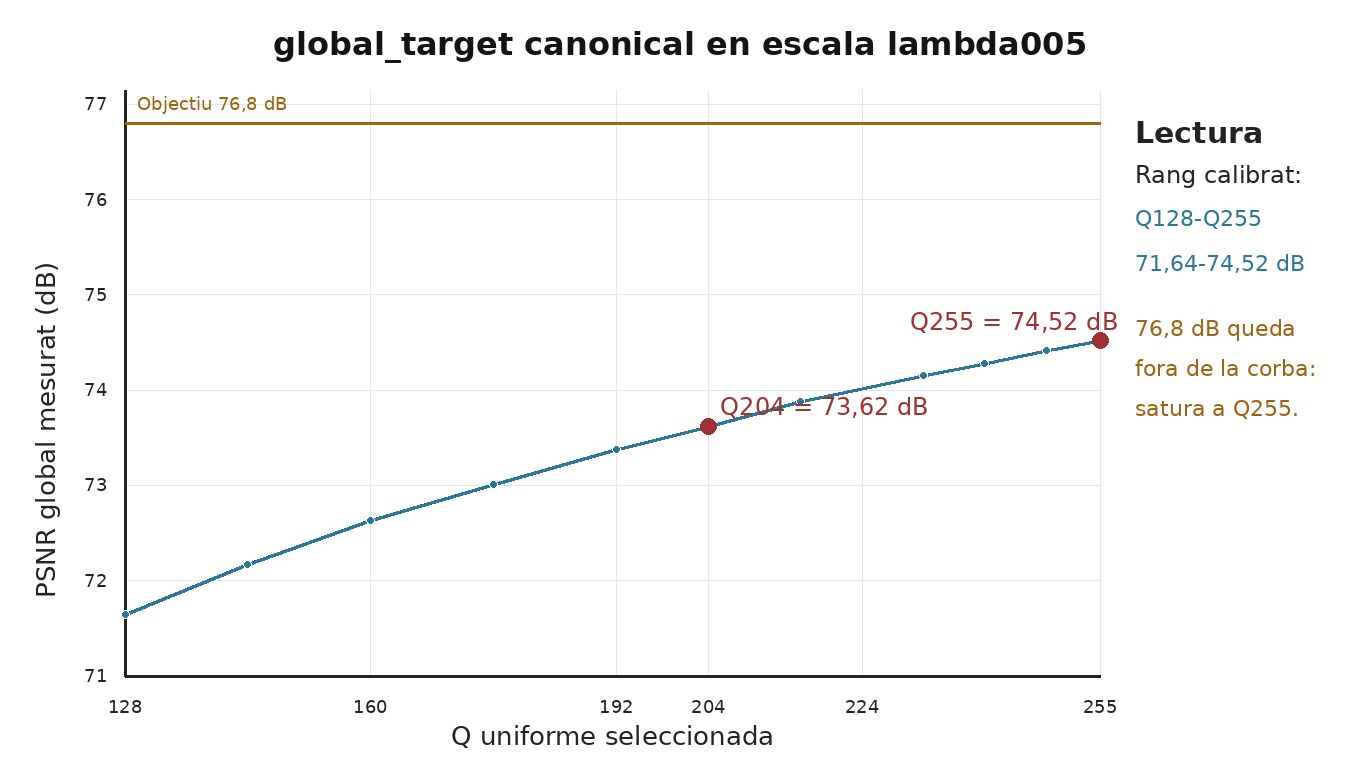
\includegraphics[width=0.90\textwidth]{global_target_lambda005_curves.png}
\caption{Corba Q--PSNR canonical de \code{global\_target} en la recalibració
\code{lambda005}. La línia horitzontal marca un objectiu de 76,8~dB. Com que la
corba canonical arriba només a 74,52~dB amb Q255, aquest target queda fora del
rang mesurat i la decisió satura.}
\label{fig:global_target_curve}
\end{figure}

La Taula~\ref{tab:global_target_precision} resumeix aquesta lectura per a
l'objectiu 76,8~dB. La idea important és que \code{global\_target} no força
qualsevol PSNR demanada: només pot seleccionar una Q dins del rang mesurat per
la calibració disponible.

\begin{table}[H]
\centering
\small
\begin{tabular}{lll}
\toprule
Magnitud & Valor & Lectura \\
\midrule
Rang PSNR Q128--Q255 & 71,64--74,52~dB & Rang calibrat canonical \\
\code{q204} & 73,62~dB & Referència uniforme dins del rang \\
Q255 & 74,52~dB & Màxim mesurat en aquesta calibració \\
Objectiu 76,8~dB & Fora de rang & Satura a Q255 \\
\bottomrule
\end{tabular}
\caption{Resultats de l'auditoria de \code{global\_target}. La població són
els punts Q128--Q255 de la calibració canonical \code{lambda005}. No es compara
contra \code{q204}: valida la conversió objectiu--Q i els seus límits.}
\label{tab:global_target_precision}
\end{table}

La conclusió és útil per a la resta de la memòria: la predicció global és
interpretable quan l'objectiu cau dins el rang calibrat, però no pot inventar
qualitat quan el target queda fora de la corba mesurada. Aquesta és la mateixa
raó per la qual les polítiques espacials es validen després amb reconstrucció,
PSNR ROI/fons i bitrate \code{.tfci}: la Q-map és una decisió de qualitat, però
el resultat final s'ha de mesurar en una execució real.

L'abast d'aquesta secció és deliberadament limitat. No és una estadística
multiimatge de \code{global\_target}, sinó una comprovació del mecanisme amb la
calibració global canònica: mostra com es transforma un objectiu en una Q
uniforme i què passa quan l'objectiu queda fora del rang mesurat. Una avaluació
estadística de precisió global requeriria repetir aquesta auditoria sobre més
retalls i objectius.

\section{Validació CSMR}\label{sec:csmr_results}

Els resultats d'aquesta secció no són prediccions de la taula de calibració. Són
execucions reals del codificador de referència de SORTENY, implementat amb
TensorFlow Compression, amb els Q-maps generats prèviament. La taula de
calibració ajuda a decidir quins valors Q escriure; CSMR mesura què passa quan
aquests valors es transformen en l'array local de qualitat i es codifiquen els
latents en un fitxer \code{.tfci}.

La mostra principal es va construir a partir del cribratge C-only: fins a cinc
casos de \code{cloud\_avoid}, fins a cinc de \code{local\_contrast}, fins a
quatre de \code{vegetation}, casos addicionals de \code{vegetation\_green} i
\code{chlorophyll}, i almenys un cas límit o negatiu quan era disponible. La
selecció no busca estimar una mitjana universal; busca cobrir situacions on la
redistribució de qualitat és plausible i casos on podria fallar.

\subsection{Correspondència L igual Q}

Els 20 retalls seleccionats generen 60 subcasos: tres polítiques per cada
retall. Tots van completar compressió i descompressió. Els 60 arrays tenien
4.096 bytes i els 60 fitxers \code{.tfci}
van produir reconstruccions amb forma $8\times512\times512$. La comprovació
clau va donar:

\begin{equation}
\code{packed\_l\_matches\_qmap}=60/60.
\end{equation}

Això confirma que l'array local de qualitat aplica per bloc els valors derivats
del Q-map C. No demostra per si sol que el preset sigui bo; demostra que
l'experiment mesura la política que s'ha sol·licitat i no una qualitat global
equivalent. Tampoc valida que la predicció de MSE de la calibració sigui exacta
en cada bloc; aquesta bondat es jutja amb PSNR, ROI/fons i bitrate \code{.tfci}.

\subsection{Comparació global de polítiques}

\begin{table}[H]
\centering
\small
\begin{tabular}{lrrrr}
\toprule
Política & Subcasos & Bitrate (bps) & PSNR global (dB) & $L=Q$ \\
\midrule
\code{q204} & 20 & 4,0602 & 74,272 & 100\% \\
\code{adaptive\_s8} & 20 & 4,0634 & 74,291 & 100\% \\
\code{focus\_bgq128} & 20 & 3,7013 & 72,369 & 100\% \\
\bottomrule
\end{tabular}
\caption{Bitrate real CSMR i PSNR global en els 20 retalls seleccionats. Cada
fila agrega 20 subcasos, un per retall. El bitrate és en bps, bits per mostra
espectral codificada.}
\label{tab:csmr_global}
\end{table}

\begin{figure}[H]
\centering
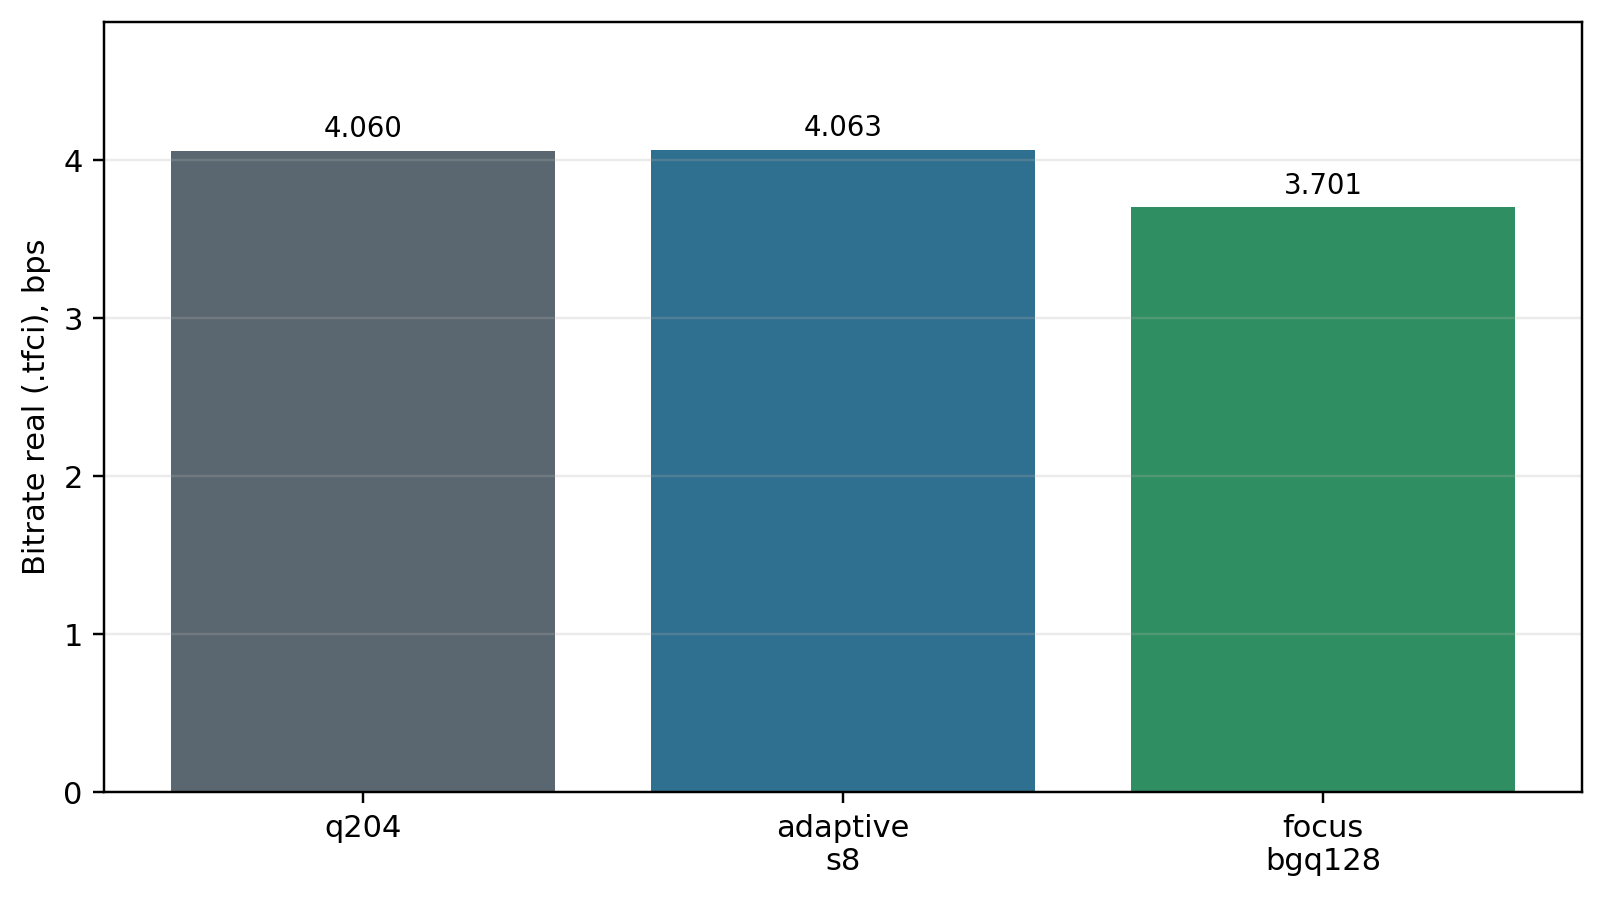
\includegraphics[width=0.72\textwidth]{csmr_policy_bitrate.png}
\caption{Bitrate mitjà dels tres controls CSMR sobre els mateixos 20 retalls.
La comparació principal és contra \code{q204}; \code{adaptive\_s8} s'inclou com
control de Q variable.}
\label{fig:csmr_policy}
\end{figure}

\code{adaptive\_s8} té pràcticament el mateix bitrate que \code{q204}: 4,0634
enfront de 4,0602~bps. El resultat no implica que el Q-map adaptatiu sigui
idèntic; conté entre Q196 i Q240. La seva mitjana és 203,994 i la redistribució
local no canvia prou l'estadística codificada per reduir la taxa global. Per
tant, \code{adaptive\_s8} és útil com a control de qualitat local, però no aporta
estalvi mesurable en aquesta mostra.

\code{focus\_bgq128} baixa a 3,7013~bps. Calculant el quocient entre mitjanes:

\begin{equation}
100\left(1-\frac{3,7013}{4,0602}\right)=8,84\%.
\end{equation}

El fitxer focus envia el 91,16\% dels bits de \code{q204}, una millora relativa
d'aproximadament $1,097\times$.

\subsection{Qualitat amb la mateixa màscara}

La mitjana de deltes per cas respecte de \code{q204} és:

\begin{equation}
\Delta\mathrm{PSNR}_{ROI}=+0,203\;\mathrm{dB},
\qquad
\Delta\mathrm{PSNR}_{fons}=-2,204\;\mathrm{dB}.
\end{equation}

Respecte d'\code{adaptive\_s8}, els valors són +0,2137 i -2,2296~dB. Les dues
referències condueixen a la mateixa conclusió: el mode conserva o millora la
ROI i obté l'estalvi degradant el fons. El PSNR global baixa perquè el fons
ocupa la major part de mostres; aquesta baixada no s'ha d'interpretar sense
separar regions.

\section{Resultats per preset}\label{sec:preset_results}

\begin{table}[H]
\centering
\scriptsize
\begin{tabular}{lrrrrr}
\toprule
Preset & Subcasos & ROI \% & Estalvi vs \code{q204} & $\Delta$ROI & $\Delta$fons \\
\midrule
\code{local\_contrast} & 5 & 10,6 & 11,68\% & +0,147 & -2,504 \\
\code{cloud\_avoid} & 5 & 20,6 & 11,56\% & +0,280 & -2,158 \\
\code{vegetation} & 4 & 11,6 & 8,56\% & +0,190 & -1,934 \\
\code{vegetation\_green} & 3 & 12,8 & 8,00\% & +0,241 & -2,221 \\
\code{chlorophyll} & 3 & 19,4 & 7,41\% & +0,147 & -2,121 \\
\bottomrule
\end{tabular}
\caption{Combinacions \code{preset + focus\_bgq128} respecte de
\code{q204}. Els deltes de PSNR són en dB i utilitzen la mateixa màscara. Cada
fila agrega els subcasos CSMR indicats.}
\label{tab:preset_csmr}
\end{table}

\begin{figure}[H]
\centering
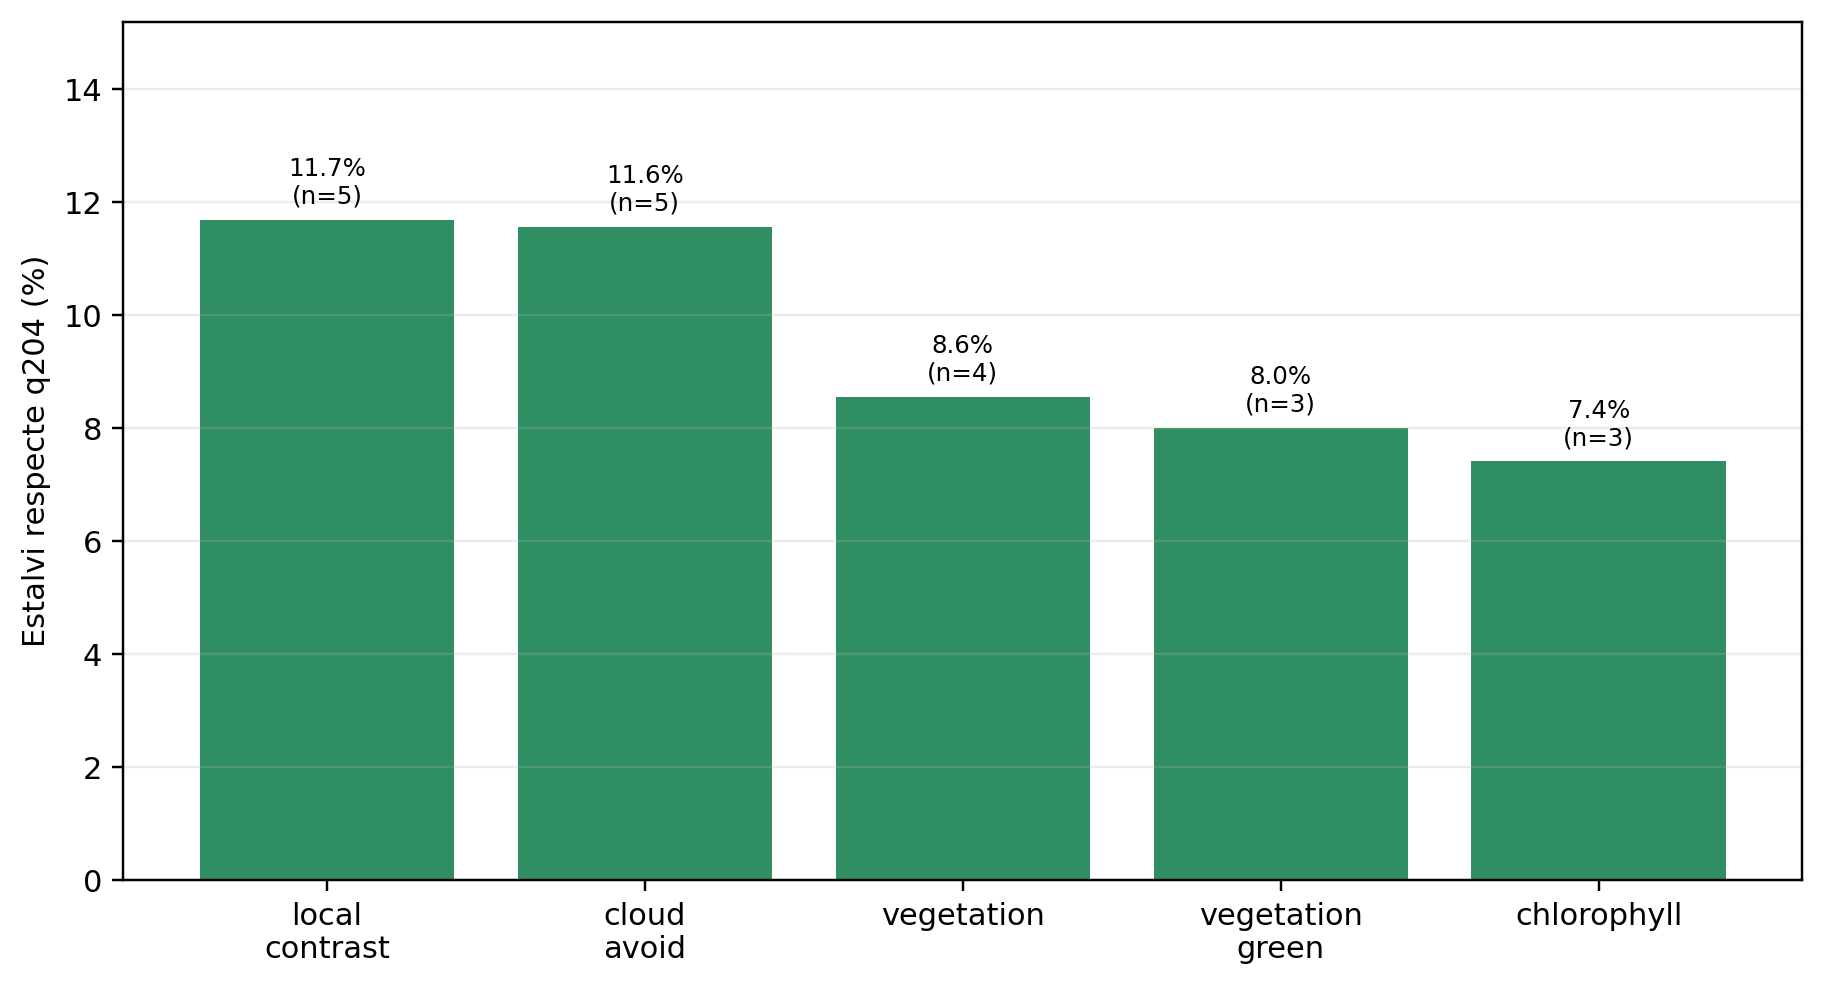
\includegraphics[width=0.86\textwidth]{csmr_savings_main_presets.png}
\caption{Estalvi mitjà per preset respecte de \code{q204}. El nombre sobre cada
barra és la mida de la mostra CSMR, no el nombre de retalls del full.}
\label{fig:preset_savings}
\end{figure}

\code{local\_contrast} i \code{cloud\_avoid} superen l'11\% de mitjana en les
seves mostres. \code{vegetation}, \code{vegetation\_green} i
\code{chlorophyll} queden entre el 7,4 i el 8,6\%. Tots presenten delta ROI
positiu i fons negatiu. Per tant, els presets no milloren una ROI manual:
milloren la qualitat de la regió que ells mateixos detecten respecte de
comprimir uniformement amb \code{q204}. Aquesta és la contribució operativa
principal.

Les mitjanes per preset no s'han de comparar sense considerar la mostra.
Cada preset es va executar en retalls seleccionats diferents. El 11,68\% de
\code{local\_contrast} no prova que sempre sigui millor que
\code{vegetation}; prova que, en els cinc casos seleccionats, la seva cobertura
permet un compromís més agressiu.

\section{Diagrames taxa--distorsió}\label{sec:rd_results}

\begin{figure}[H]
\centering
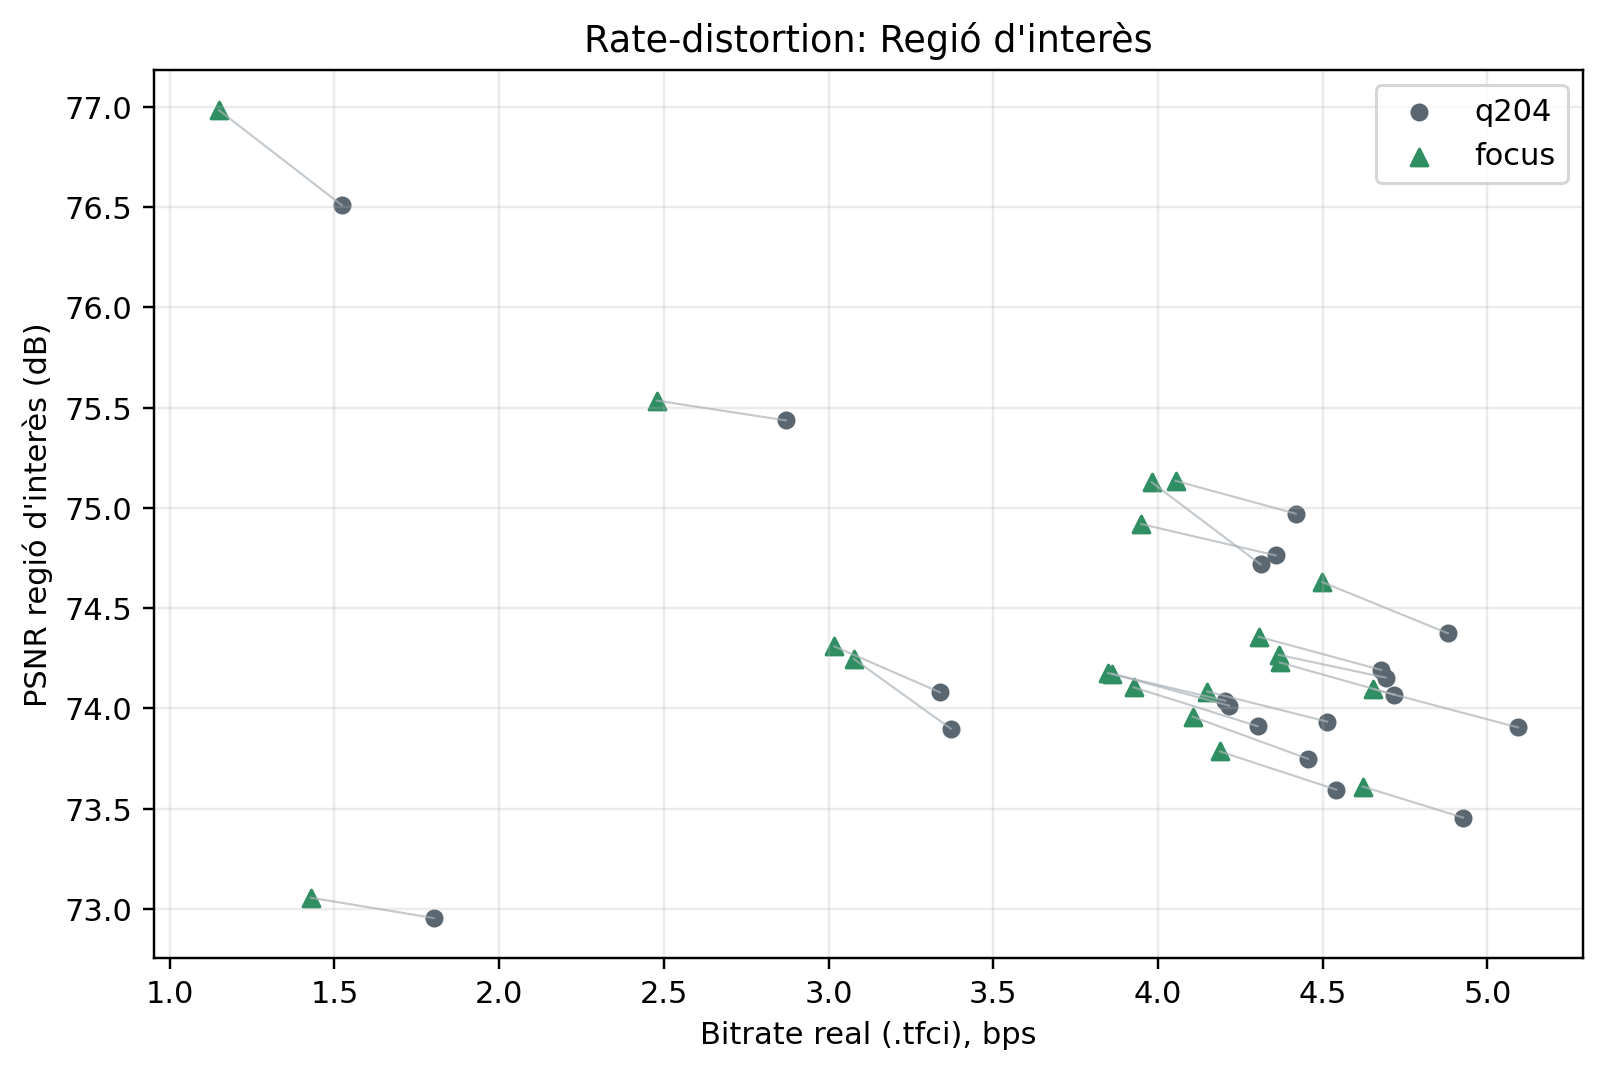
\includegraphics[width=0.88\textwidth]{rd_roi_q204_focus.png}
\caption{Diagrama taxa--distorsió dins la ROI. Cada parella unida correspon al
mateix retall i la mateixa màscara. Un desplaçament a l'esquerra i amunt indica
menys bitrate i més PSNR ROI.}
\label{fig:rd_roi}
\end{figure}

La Figura~\ref{fig:rd_roi} mostra que la majoria de punts focus es desplacen a
l'esquerra i lleugerament amunt respecte de \code{q204}. La dispersió vertical
entre retalls és molt més gran que el delta d'una política, perquè les escenes
tenen errors base diferents. Per això les línies per parella són més
informatives que comparar núvols de punts sense correspondència.

\begin{figure}[H]
\centering
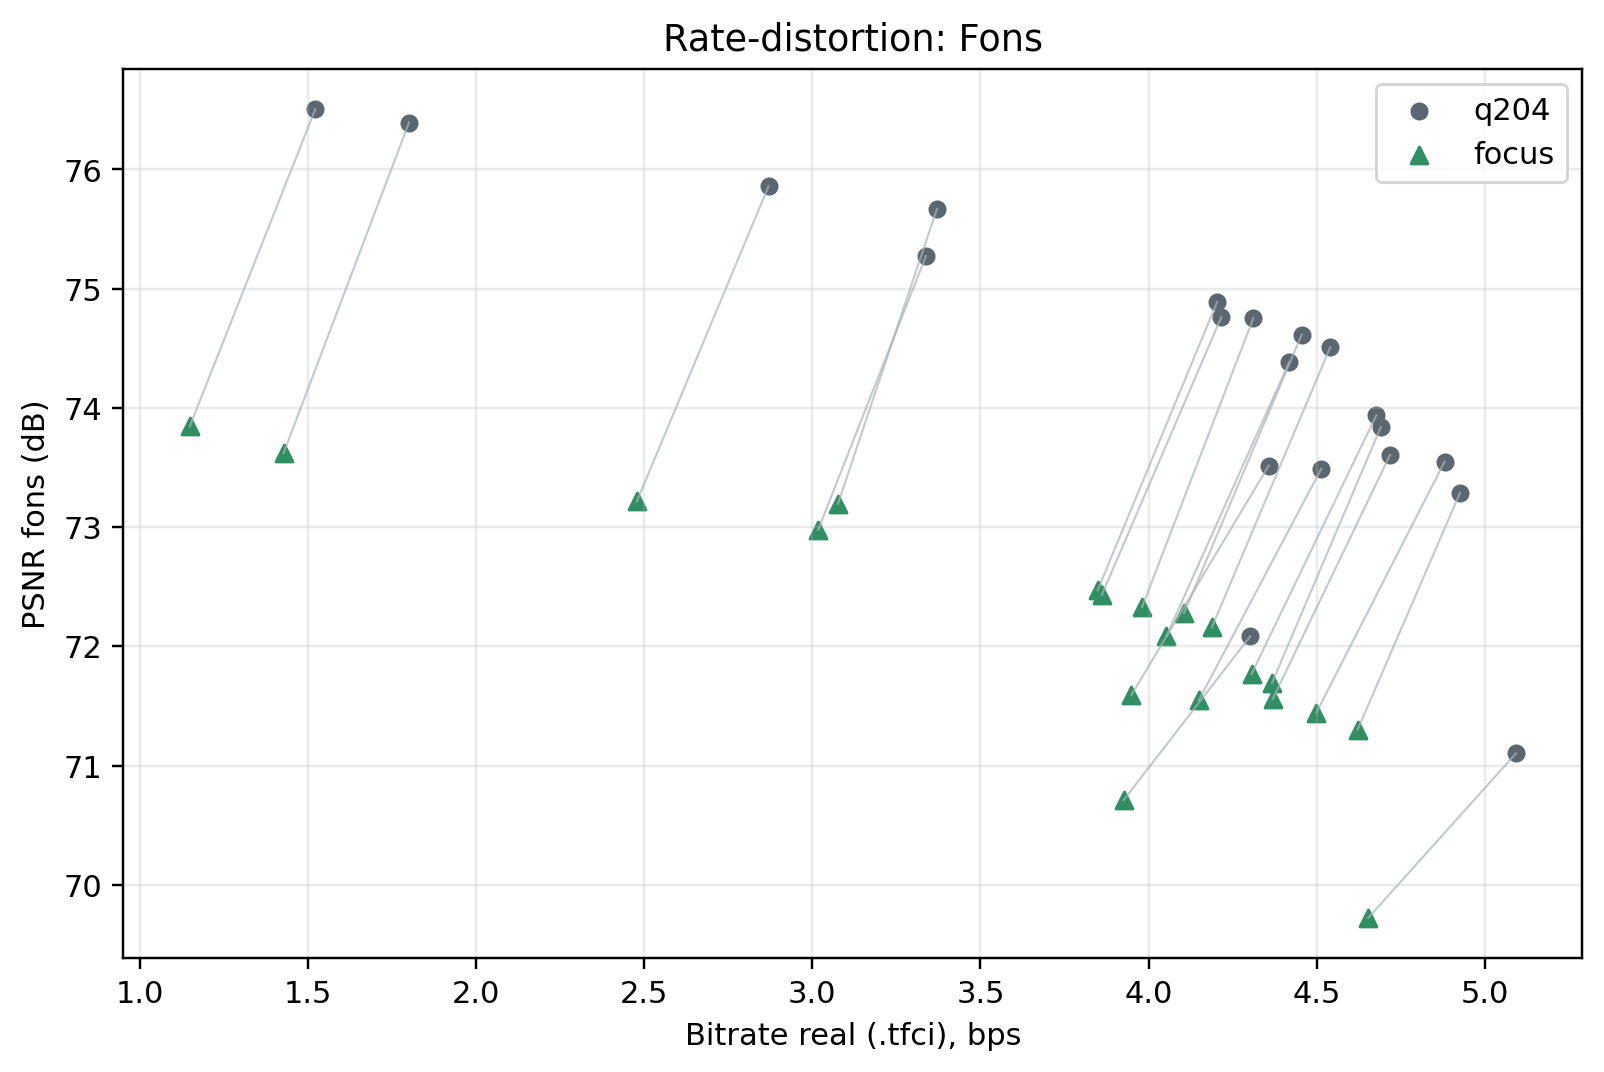
\includegraphics[width=0.88\textwidth]{rd_background_q204_focus.png}
\caption{Diagrama taxa--distorsió al fons. El moviment esperat és cap a
l'esquerra i avall: menys bitrate a canvi de més distorsió en la regió no
prioritària.}
\label{fig:rd_background}
\end{figure}

Al fons, Figura~\ref{fig:rd_background}, el desplaçament cap avall és clar.
Aquest resultat evita una interpretació equivocada: focus no millora tota la
imatge mentre comprimeix més. Redistribueix un pressupost de qualitat.

\section{Modes experimentals}\label{sec:experimental_results}

L'auditoria experimental va completar 30 de 30 subcasos i va conservar $L=Q$
en tots. Cada fila de la Taula~\ref{tab:experimental} compara el mode avaluat
contra \code{q204} del mateix retall i la mateixa màscara ROI/fons.

\begin{table}[H]
\centering
\small
\begin{tabular}{lrrrrl}
\toprule
Mode avaluat & Subcasos & ROI \% & Estalvi & $\Delta$ROI & Lectura \\
\midrule
\code{high\_ndvi + focus\_bgq128} & 3 & 20,4 & 6,54\% & +0,165 & Candidat útil \\
\code{low\_ndvi + focus\_bgq128} & 3 & 4,9 & 9,05\% & +0,120 & ROI massa petita \\
\code{dark\_regions + focus\_bgq128} & 3 & 62,4 & 1,99\% & +0,384 & ROI massa ampla \\
\code{water\_body + focus\_bgq128} & 1 & 10,1 & 11,18\% & +0,158 & Una sola mostra \\
\bottomrule
\end{tabular}
\caption{CSMR dels llindars experimentals. Estalvi i PSNR es calculen respecte
de \code{q204}; el nombre de subcasos limita la força de cada conclusió.}
\label{tab:experimental}
\end{table}

\begin{figure}[H]
\centering
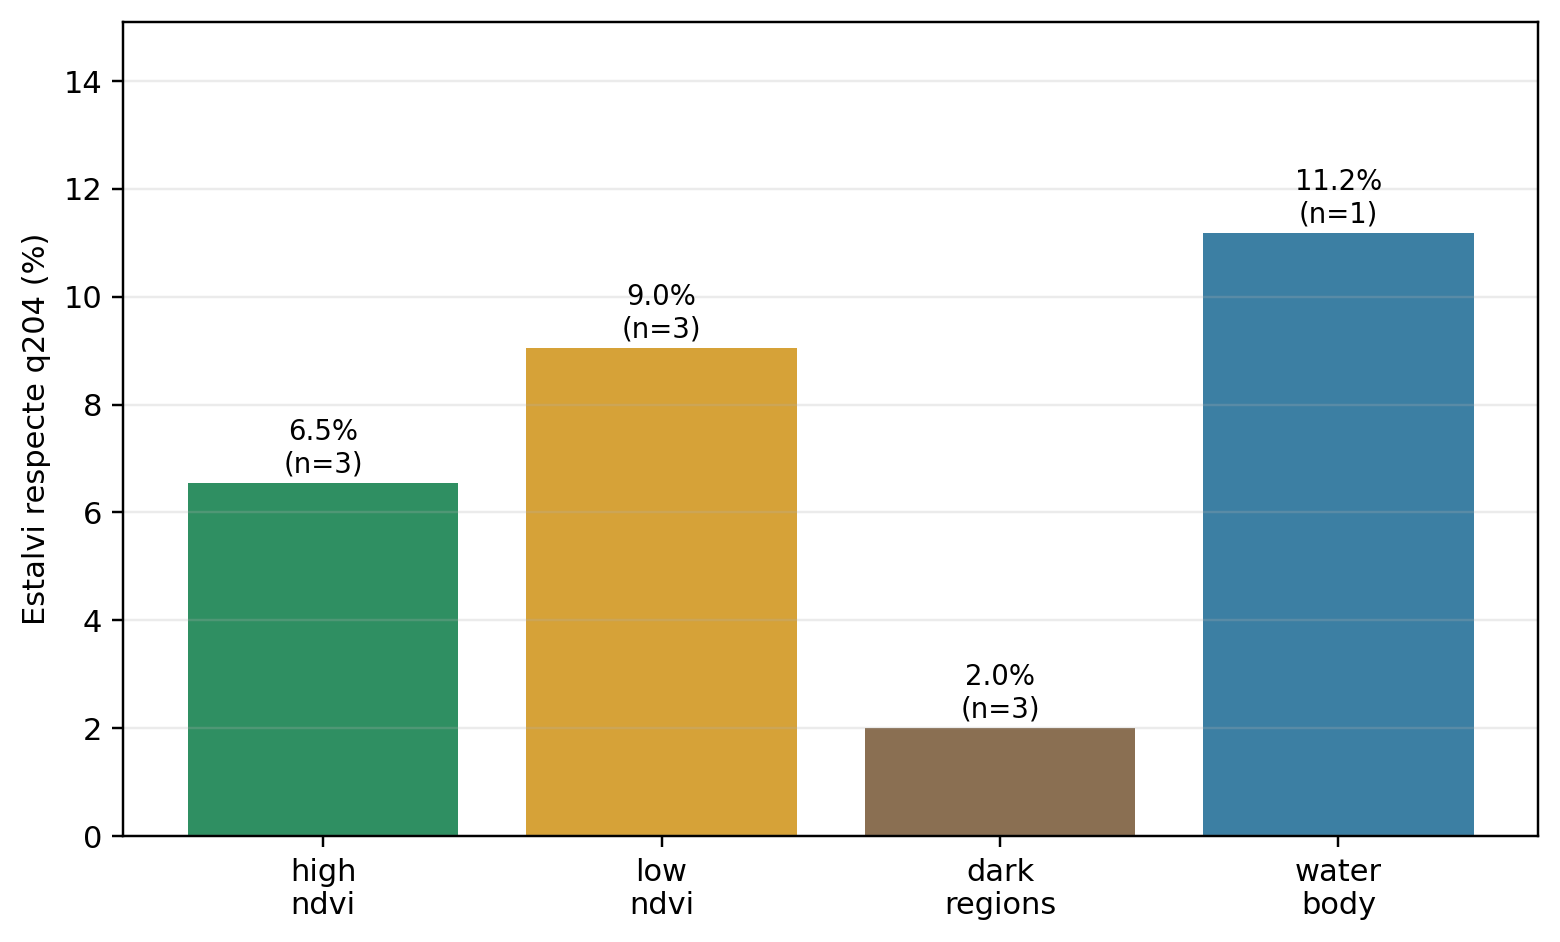
\includegraphics[width=0.74\textwidth]{csmr_experimental_savings.png}
\caption{Estalvi dels presets experimentals. La mida de mostra s'indica sobre
cada barra i limita la força de la conclusió.}
\label{fig:experimental}
\end{figure}

\code{high\_ndvi} és el resultat més equilibrat: tres casos mid-roi i un
estalvi del 6,54\%. Per això es va promocionar a la configuració operativa del
benchmark Raspberry. \code{low\_ndvi} comprimeix més, però dos dels tres casos
tenen només 0,78\% de ROI; una regió tan dispersa és més vulnerable a
l'efecte dels blocs veïns. \code{dark\_regions} conserva ROI, però dedica
qualitat alta a gairebé dos terços de la imatge i deixa poc fons per degradar.

El cas \code{water\_body} requereix una precisió metodològica. Al full original
amb llindar 0,30, 119 dels 120 retalls no tenien ROI i un tenia una ROI de
0,098\%. L'optimització va reduir el llindar a 0,10, però només un crop
representatiu d'aigua havia estat seleccionat per aquell barratge i va passar
a CSMR. Per tant, una mostra no significa que la resta del dataset sigui tot
aigua o tota no-ROI amb el llindar nou; significa que l'experiment no va
regenerar els 120 retalls a 0,10. El 11,18\% és prometedor, però insuficient
per generalitzar.

\section{Preserve-roi}\label{sec:preserve_results}

La prova CSMR de \code{preserve-roi} va completar 78 subcasos. La
Taula~\ref{tab:preserve_cloud} mostra dos casos \code{cloud\_avoid} compartits
per les tres polítiques.

\begin{table}[H]
\centering
\small
\begin{tabular}{lrrr}
\toprule
Política & Estalvi vs \code{q204} & $\Delta$ROI vs \code{q204} &
$\Delta$fons vs \code{q204} \\
\midrule
\code{focus\_bgq128} & 17,06\% & +0,351 & -2,478 \\
\code{preserve Q240/Q128} & 15,88\% & +0,626 & -2,480 \\
\code{preserve Q255/Q128} & 15,30\% & +1,024 & -2,476 \\
\bottomrule
\end{tabular}
\caption{Compromís de \code{preserve-roi} en dos casos \code{cloud\_avoid}.
Els deltes són dB amb màscara comuna i el baseline és \code{q204}.}
\label{tab:preserve_cloud}
\end{table}

\begin{figure}[H]
\centering
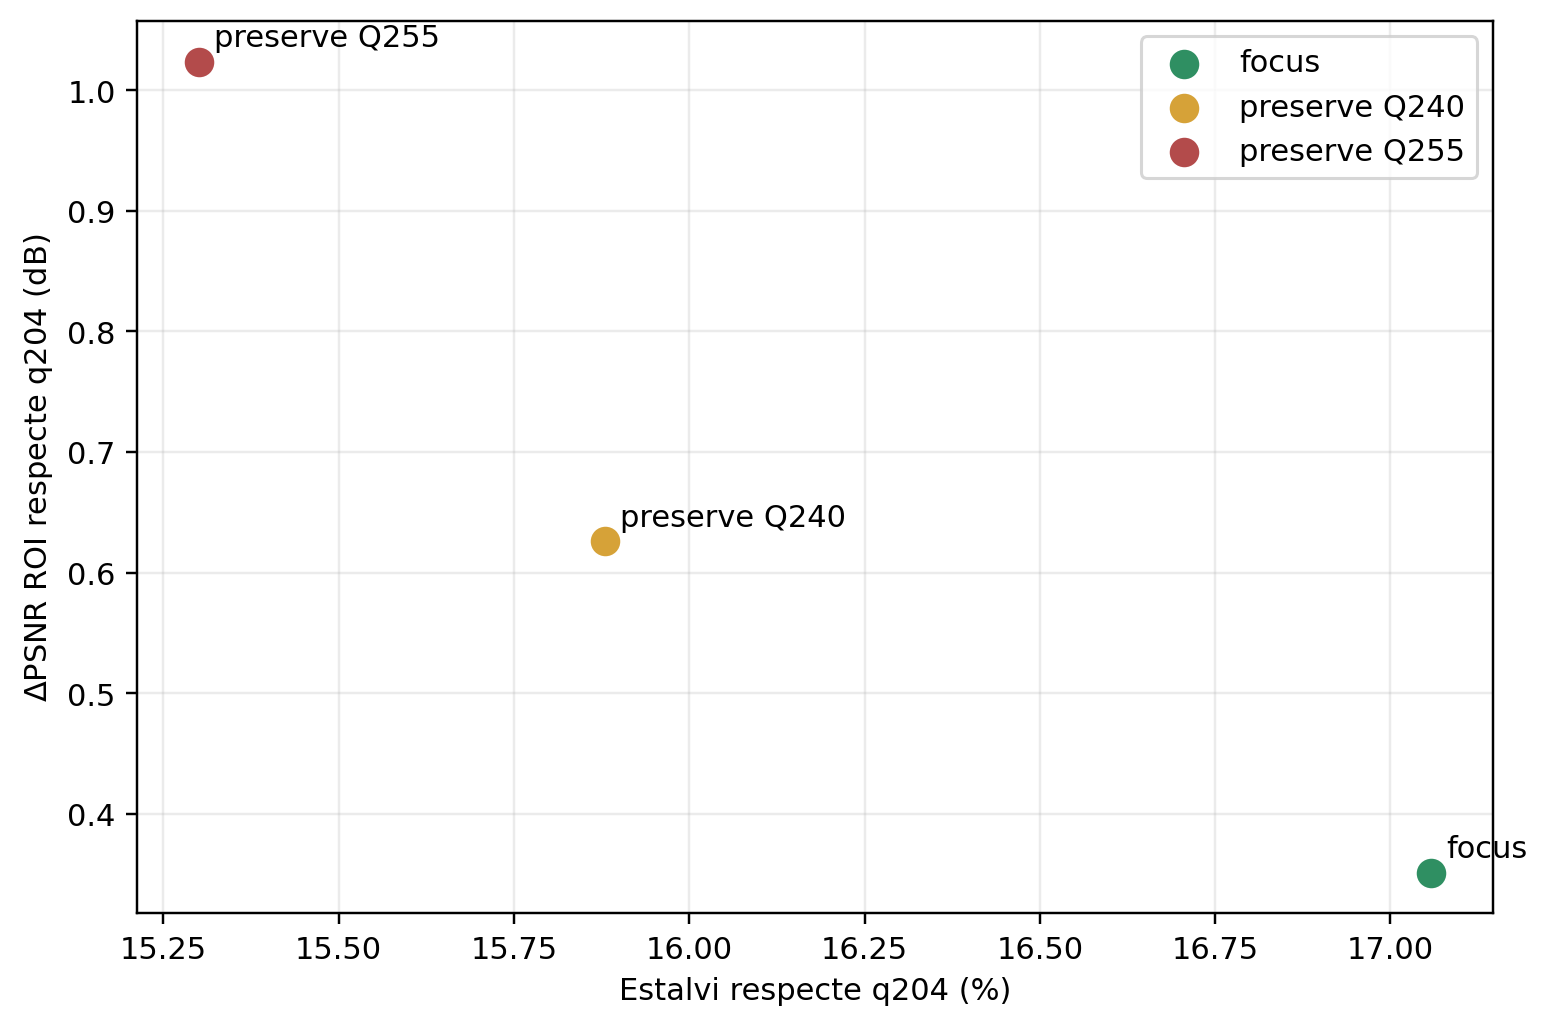
\includegraphics[width=0.76\textwidth]{preserve_roi_tradeoff.png}
\caption{Intercanvi entre estalvi i preservació de ROI. La posició més a la
dreta afavoreix compressió; la posició més alta afavoreix qualitat ROI.}
\label{fig:preserve_tradeoff}
\end{figure}

El resultat respon a objectius diferents. \code{focus} és preferible si es
prioritza bitrate. Q255 és preferible si es vol assegurar una ROI clarament
millor que \code{q204}. Q240 és un compromís intermedi. No hi ha una política
dominant en les dues dimensions: la decisió depèn de si la missió valora més
baixar volum de dades o protegir la regió seleccionada.

\section{Evidència visual}\label{sec:visual_results}

Els panells següents tenen quatre columnes:

\begin{enumerate}[leftmargin=*]
  \item composició RGB de l'entrada;
  \item màscara del preset superposada en verd;
  \item Q-map ampliat, on colors clars indiquen Q més alta;
  \item error absolut amplificat per fer visible la seva distribució.
\end{enumerate}

L'error amplificat no és l'aspecte de la reconstrucció. La multiplicació visual
serveix per localitzar on es concentra la pèrdua. La imatge reconstruïda
completa acostuma a semblar gairebé igual que l'original; la prova quantitativa
és el PSNR i la prova espacial és el Q-map.

\begin{table}[H]
\centering
\scriptsize
\begin{tabular}{lrrrr}
\toprule
Panell visual & ROI \% & Estalvi vs \code{q204} & $\Delta$ROI &
$\Delta$fons \\
\midrule
\code{cloud\_avoid + focus} & 15,1 & 24,5\% & +0,474 & -2,660 \\
\code{local\_contrast + focus} & 10,1 & 20,7\% & +0,101 & -2,773 \\
\code{vegetation + focus} & 10,5 & 9,4\% & +0,156 & -1,921 \\
\code{high\_ndvi + focus} & 10,9 & 8,1\% & +0,161 & -2,297 \\
\code{cloud\_avoid + preserve Q240} & 15,1 & 22,9\% & +0,624 & -2,663 \\
\bottomrule
\end{tabular}
\caption{Lectura quantitativa dels panells visuals. El baseline és
\code{q204}; els deltes de PSNR són en dB amb la mateixa màscara ROI/fons que
mostra cada panel.}
\label{tab:visual_metrics}
\end{table}

\begin{figure}[H]
\centering
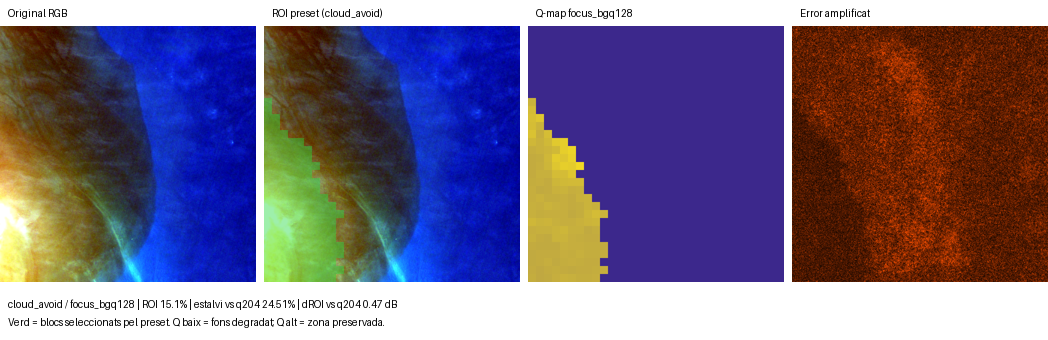
\includegraphics[width=\textwidth]{01_main_cloud_avoid_focus_bgq128.png}
\caption{\code{cloud\_avoid + focus\_bgq128}. El preset selecciona la ROI
detectada com a zona no ennuvolada o útil i el fons queda a Q128. En aquest
crop, la cobertura és 15,1\%, l'estalvi respecte de \code{q204} és 24,5\% i la
ROI millora 0,47~dB.}
\label{fig:visual_cloud}
\end{figure}

La Figura~\ref{fig:visual_cloud} és un cas especialment favorable, no la
mitjana del preset. La frontera es veu esglaonada perquè la decisió es pren en
blocs de $16\times16$. El Q-map mostra variació dins la ROI perquè \code{focus}
parteix d'\code{adaptive\_s8}; no és un nivell fix.

\begin{figure}[H]
\centering
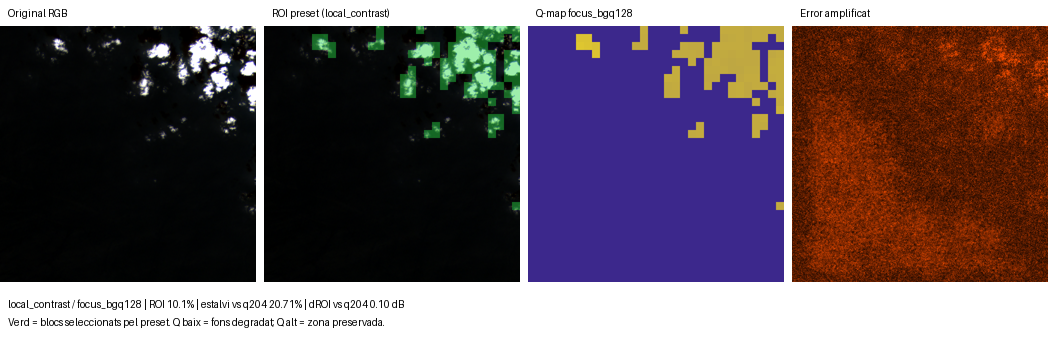
\includegraphics[width=\textwidth]{02_main_local_contrast_focus_bgq128.png}
\caption{\code{local\_contrast + focus\_bgq128}. Les zones amb més variació
visible reben la qualitat adaptativa reforçada.}
\label{fig:visual_contrast}
\end{figure}

\code{local\_contrast} no etiqueta una coberta física. La màscara de la
Figura~\ref{fig:visual_contrast} indica on la desviació visible supera 0,035.
És útil per conservar vores i textures, però la missió hauria de decidir si
aquesta prioritat és coherent amb l'aplicació final.

\begin{figure}[H]
\centering
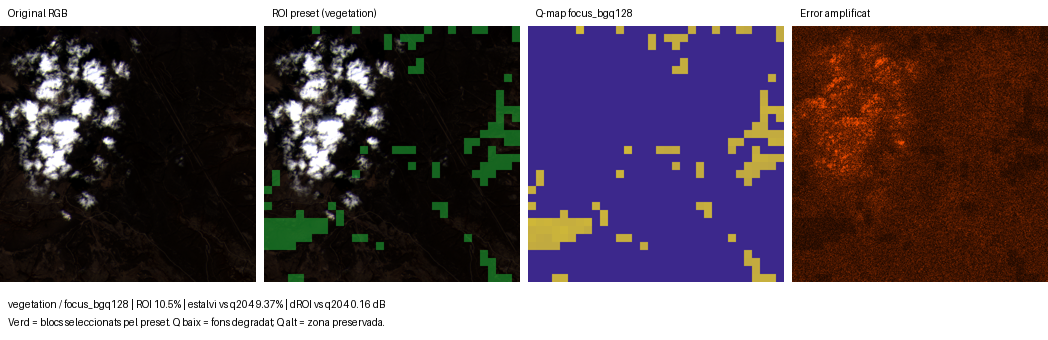
\includegraphics[width=\textwidth]{03_main_vegetation_focus_bgq128.png}
\caption{\code{vegetation + focus\_bgq128}. La màscara NDVI protegeix blocs
vegetats i deixa la resta a Q128.}
\label{fig:visual_vegetation}
\end{figure}

La Figura~\ref{fig:visual_vegetation} mostra una selecció més fragmentada.
Aquest tipus de geometria és rellevant perquè el camp receptiu travessa blocs
veïns. Els resultats indiquen ROI conservada en la mostra CSMR, però regions
encara més petites podrien requerir dilatar la màscara o utilitzar
\code{preserve-roi}.

\begin{figure}[H]
\centering
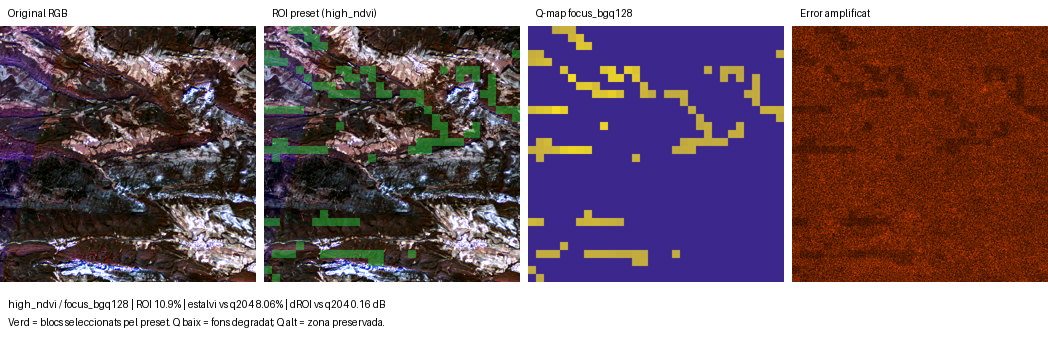
\includegraphics[width=\textwidth]{04_experimental_high_ndvi_focus_bgq128.png}
\caption{\code{high\_ndvi + focus\_bgq128}. Exemple del preset experimental que
va obtenir tres casos mid-roi consistents.}
\label{fig:visual_high_ndvi}
\end{figure}

\code{high\_ndvi} és més restrictiu que \code{vegetation}. La figura permet
entendre per què els dos presets poden coexistir: no són dues polítiques, sinó
dos nivells de selecció de la mateixa magnitud espectral.

\begin{figure}[H]
\centering
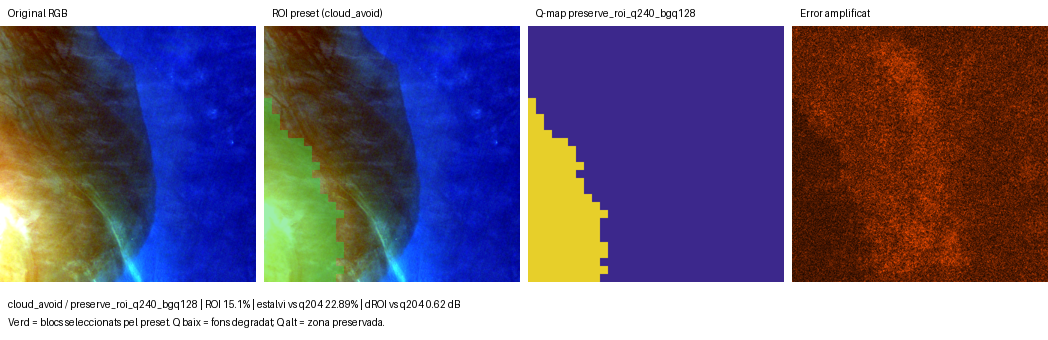
\includegraphics[width=\textwidth]{05_preserve_cloud_avoid_preserve_roi_q240_bgq128.png}
\caption{\code{cloud\_avoid + preserve-roi Q240/Q128}. La ROI té un color
uniforme perquè Q240 és fixa; aquesta és la diferència visual amb el Q-map
adaptatiu de la Figura~\ref{fig:visual_cloud}.}
\label{fig:visual_preserve}
\end{figure}

\section{Abast de la lectura}\label{sec:statistical_reading}

Les comparacions CSMR són aparellades per retall: cada resultat focus,
experimental o preserve-roi es compara amb el \code{q204} del mateix crop i la
mateixa màscara. Tot i això, les taules combinen poblacions diferents. El full
C-only conté 120 retalls; el CSMR principal en conté 20; les taules per preset
agreguen entre tres i cinc subcasos; i les auditories experimentals provenen de
mostres separades. Per això els percentatges s'han de llegir com a evidència de
mecanisme i de compromís, no com una mitjana universal de missió.

\section{Resultats que informen l'usuari}\label{sec:user_implications}

La geometria de la ROI canvia el valor del sistema. La
Taula~\ref{tab:user_roi_cases} resumeix les decisions derivades.

\begin{table}[H]
\centering
\small
\begin{tabularx}{\textwidth}{p{3.0cm}p{4.0cm}X}
\toprule
Cobertura observada & Conseqüència & Decisió recomanada \\
\midrule
ROI buida & Tot rep qualitat de fons; no es preserva cap regió. & Usar
\code{q204},
un altre preset o no transmetre si la missió ho permet. \\
ROI molt petita i dispersa & El camp receptiu travessa blocs veïns i pot
degradar la regió tot i el Q alt. & Dilatar màscara, usar preserve-roi o revisar
el llindar. \\
ROI intermèdia & Hi ha prou ROI i fons per redistribuir qualitat. & Focus és
el candidat principal si els deltes CSMR són favorables. \\
ROI molt ampla & Queda poc fons on estalviar i el bitrate s'apropa al control. &
Usar un llindar més selectiu o \code{q204}. \\
ROI total & Tots els blocs són prioritaris; no hi ha redistribució espacial. &
Usar qualitat global o preserve només si es vol Q alta uniforme. \\
\bottomrule
\end{tabularx}
\caption{Implicacions operatives de la cobertura produïda pel preset.}
\label{tab:user_roi_cases}
\end{table}

Aquestes regles mostren per què un preset no s'ha de jutjar només pel bitrate.
\code{low\_ndvi} aconsegueix estalvi en tres casos, però la ROI mitjana és
petita; \code{dark\_regions} conserva ROI, però n'ocupa massa; \code{water\_body}
té un cas prometedor sense cobertura suficient. El mode útil no és el que
produeix el fitxer més petit, sinó el que selecciona una regió coherent amb la
missió i la conserva a un cost assumible.

\subsection{Focus davant preserve-roi}

La comparació de la Taula~\ref{tab:preserve_cloud} permet formular una regla
d'usuari. Si el downlink és el recurs dominant, focus ofereix més estalvi. Si
la pèrdua d'una estructura ROI és més costosa que enviar alguns bits
addicionals, Q240 o Q255 proporcionen més marge. La selecció no s'ha
d'automatitzar només amb una mitjana global; forma part dels requisits de
missió.

Els resultats d'aquest capítol mostren el compromís entre qualitat espacial i
bitrate real. La pregunta següent és si aquest compromís té un cost assumible en
hardware de baix recurs; això es tracta al Capítol~\ref{ch:bord}.

\thispagestyle{empty}

\cleardoublepage
% !TEX root = ../main.tex
\chapter{Execució a bord i discussió}\label{ch:bord}
\fancyhead[RE]{\slshape \textsf{Capítol \thechapter.\ Execució a bord}}
\fancyhead[LO]{\slshape \textsf{\nouppercase \rightmark}}

\section{Per què cal avaluar el processament a bord}\label{sec:onboard_motivation}

La utilitat del control espacial de qualitat depèn de poder prendre la decisió
abans de transmetre les dades. En una estació terrestre seria possible aplicar
un segmentador més gran, revisar manualment la imatge o repetir la compressió.
En canvi, a bord hi ha restriccions de còmput, memòria, energia i temps de
contacte. Per aquest motiu, no és suficient demostrar que una màscara produeix
menys bitrate: també cal mesurar el cost de generar-la i d'executar el còdec.

L'arquitectura escollida separa dos costos:

\begin{enumerate}[leftmargin=*]
  \item \textbf{decisió espacial}: lectura del RAW, càlcul de l'índex o
  descriptor del preset i escriptura del Q-map;
  \item \textbf{transformació neuronal}: anàlisi espectral i espacial,
  modulació, quantització i generació dels latents.
\end{enumerate}

Aquesta separació és rellevant des de la perspectiva de sistema. Si el primer
cost fos comparable al segon, l'estalvi de bits podria no compensar el càlcul
addicional. Si és molt menor, es poden oferir diversos presets sense alterar
de manera apreciable la latència del còdec.

\section{Plataforma i abast de la demostració}\label{sec:rpi_platform}

La plataforma és una Raspberry Pi 3 Model B+ amb quatre nuclis ARM
Cortex-A53 a 1,4~GHz i aproximadament 1~GiB de memòria. El sistema utilitza
Linux de 64 bits i compila el codi amb GCC, \code{-O3}, OpenMP i opcions
específiques per a Cortex-A53. Aquesta família de processadors és pertinent per
estudiar codi de baix recurs i comparteix característiques amb ordinadors de
bord basats en ARM, però la Raspberry no és maquinari qualificat per a vol.
Aspectes com radiació, redundància, temps real, consum elèctric, interfícies del
sensor i certificació queden fora de la demostració. La comparació correcta és,
per tant, de \emph{representativitat computacional}, no d'equivalència de vol
\cite{raspberry2018brief,schwaller2017a53,serra2024c3satp}.

El bundle d'assaig és autocontingut: inclou codi C, pesos, calibració, sis
retalls RAW, llindars i scripts. No instal·la TensorFlow, NumPy ni paquets del
sistema. Cada execució desa \code{/usr/bin/time -v}, RSS màxim, temperatura,
estat de throttling, arguments, hashes i mides. Aquesta decisió limita les
diferències entre l'entorn local i la placa i permet reconstruir posteriorment
les mètriques al PC.

\begin{table}[H]
\centering
\small
\begin{tabular}{ll}
\toprule
Element & Configuració mesurada \\
\midrule
CPU & 4 $\times$ ARM Cortex-A53, fins a 1,4~GHz \\
Memòria & 909~MiB visibles pel sistema \\
Entrada & 8 bandes, $512\times512$, \code{uint16}, 4.194.304 bytes \\
Compilació & GCC \code{-O3 -fopenmp -mcpu=cortex-a53} \\
Paral·lelisme final & 4 fils OpenMP \\
Mostra & 6 retalls $\times$ 11 polítiques = 66 execucions \\
Instrumentació & \code{/usr/bin/time -v}, \code{vcgencmd}, hashes i logs \\
\bottomrule
\end{tabular}
\caption{Condicions principals del benchmark Raspberry optimitzat. La mostra
correspon a sis retalls i onze polítiques amb quatre fils.}
\label{tab:rpi_setup}
\end{table}

\section{Escalat inicial amb OpenMP}\label{sec:rpi_scaling}

Abans de modificar els kernels es va executar la mateixa càrrega amb un, dos i
quatre fils. Els valors de la Taula~\ref{tab:rpi_scaling} són mitjanes per una
imatge i una política; no són el temps de tot el dataset. Cada entrada conté
2.097.152 mostres espectrals.

\begin{table}[H]
\centering
\small
\begin{tabular}{rrrrr}
\toprule
Fils & Compressió (s) & Descompressió (s) & Total (s) & Speedup total \\
\midrule
1 & 561,73 & 413,22 & 974,96 & 1,00$\times$ \\
2 & 368,20 & 270,85 & 639,05 & 1,53$\times$ \\
4 & 316,43 & 247,69 & 564,12 & 1,73$\times$ \\
\bottomrule
\end{tabular}
\caption{Escalat inicial mitjà per retall i política. El speedup es calcula
respecte d'un fil.}
\label{tab:rpi_scaling}
\end{table}

Quatre fils redueixen el temps total un 42,1\% respecte d'un fil. L'escalat no
és lineal: un speedup ideal seria $4\times$, però s'obté $1,73\times$. Hi
contribueixen les regions serials, el cost de crear equips OpenMP, la pressió
sobre memòria i l'amplada de banda compartida. Tot i això, quatre fils és la
configuració operativa perquè és la més ràpida de les tres i no produeix
errors ni falta de memòria.

\subsection{Lectura amb la llei d'Amdahl}

La llei d'Amdahl no és una hipòtesi del projecte, sinó una eina clàssica per
interpretar per què un programa no accelera linealment quan s'afegeixen nuclis
\cite{amdahl1967}. En aquest cas serveix per donar context al resultat OpenMP:
si una part del temps no escala amb els fils, el speedup total queda limitat
encara que algunes funcions internes sí siguin paral·leles. La forma utilitzada
expressa el speedup amb $p$ fils com:

\begin{equation}
S(p)=\frac{1}{f+(1-f)/p},
\end{equation}

on $f$ és la fracció serial o, més precisament, la fracció aparent que no escala
en aquesta mesura. Substituint $S(4)=974,96/564,12=1,728$, s'obté:

\begin{equation}
f\simeq
\frac{1/S(4)-1/4}{1-1/4}=0,44.
\end{equation}

Aquest 44\% no és una mesura directa d'una funció serial del codi. Agrupa I/O,
regions no paral·lelitzades, ample de banda de memòria, sincronització, cost
d'OpenMP i possibles variacions de freqüència. La lectura útil és que afegir més
fils al mateix codi no pot donar un speedup proper al nombre de nuclis. Cal
reduir el treball de les capes o canviar la jerarquia de memòria.

La millora incremental ataca part d'aquesta fracció en GDN/IGDN,
depth-to-space i transformada espectral. Les convolucions continuen sent el
volum principal d'operacions, però ja disposaven de paral·lelisme per canals.
Una optimització posterior hauria de perfilar cache misses, vectorització i
reutilització de kernel abans d'afegir directives OpenMP indiscriminadament.

\section{Optimització incremental del C}\label{sec:c_optimization}

L'optimització no es va fer canviant el model, els pesos o l'ordre aritmètic
intern. Es van introduir tres canvis separats i es va executar una auditoria de
paritat després de cadascun:

\begin{description}[leftmargin=3.7cm,style=nextline]
  \item[GDN i IGDN] Paral·lelisme sobre píxels, mantenint privat el denominador
  de cada fil i l'ordre d'acumulació sobre canals.
  \item[Depth-to-space] Paral·lelisme sobre canals de sortida. Aquesta operació
  només reordena memòria i ha de ser exacta bit a bit.
  \item[Transformada espectral] Paral·lelisme sobre píxels, mantenint l'ordre
  intern de les bandes per no alterar l'aritmètica en coma flotant.
\end{description}

Abans dels canvis es va crear una golden baseline amb Q-map, bitstream,
reconstrucció, hashes i temps. L'auditor compara Q-map byte a byte i
reconstrucció RAW byte a byte. Si aparegués una diferència, també calcularia
error màxim, MAE, MSE i PSNR. En les 66 parelles Raspberry de la comparació
final no es va registrar cap fallada de paritat.

\subsection{Temps abans i després}

\begin{table}[H]
\centering
\small
\begin{tabular}{lrrrr}
\toprule
Etapa & Baseline (s) & Optimitzat (s) & Reducció (s) & Speedup \\
\midrule
Compressió & 316,43 & 261,32 & 55,11 & 1,211$\times$ \\
Descompressió & 247,69 & 206,80 & 40,89 & 1,198$\times$ \\
Total & 564,12 & 468,13 & 96,00 & 1,205$\times$ \\
\bottomrule
\end{tabular}
\caption{Temps mitjans per retall i política amb quatre fils. Les 66 parelles
comparen les mateixes entrades i Q-maps.}
\label{tab:rpi_optimized_time}
\end{table}

La millora total mitjana és $1,205\times$, equivalent a una reducció del
17,0\% del temps. La Figura~\ref{fig:rpi_speedup} mostra que el resultat és
estable entre polítiques: els speedups totals se situen aproximadament entre
$1,20\times$ i $1,21\times$. Això és coherent amb el fet que les polítiques
només canvien el Q-map; les capes convolucionals dominants són les mateixes.

\begin{figure}[H]
\centering
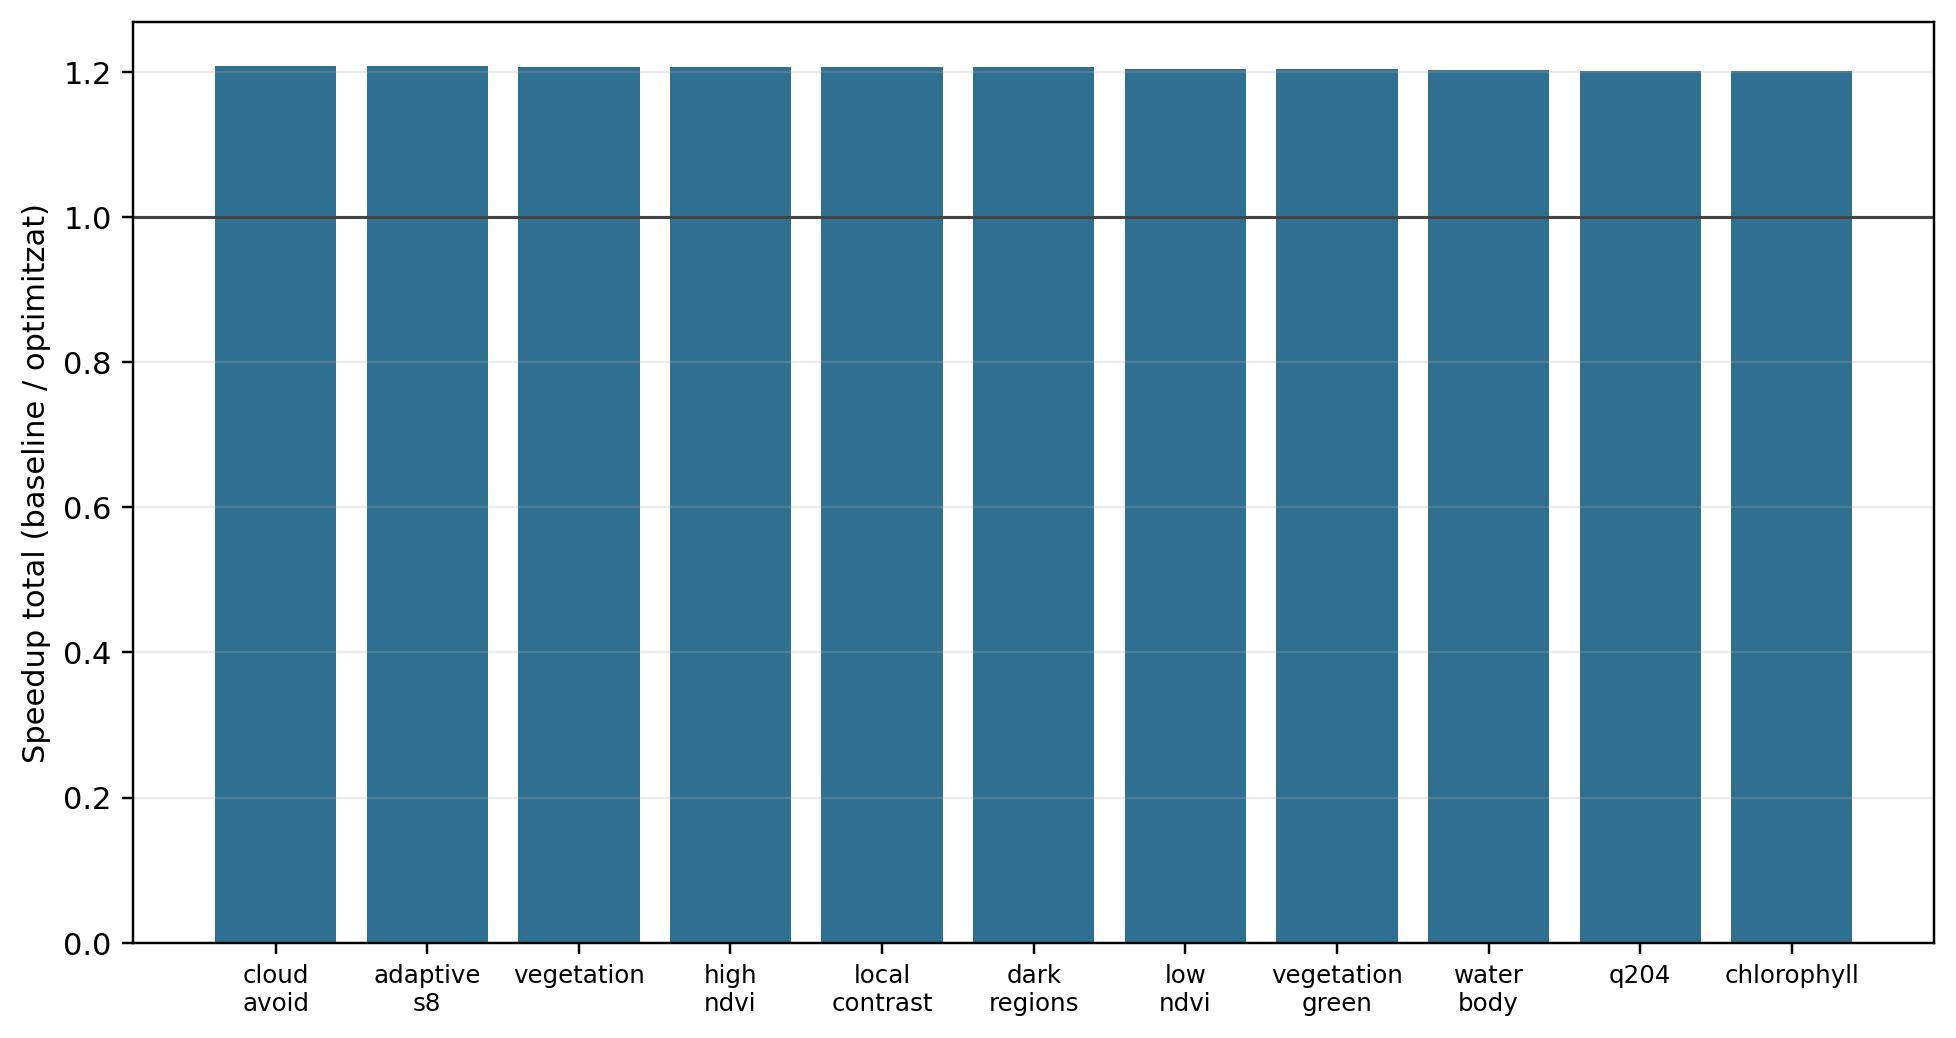
\includegraphics[width=0.88\textwidth]{raspberry_speedup_by_mode.png}
\caption{Speedup total de la versió C optimitzada per política, sempre amb
quatre fils. La línia $1\times$ representa absència de millora.}
\label{fig:rpi_speedup}
\end{figure}

El RSS màxim mitjà del compressor passa de 90.136~KiB a 89.505~KiB. Per tant,
el paral·lelisme introduït no exigeix una còpia completa del tensor per fil i
no augmenta la memòria de manera rellevant. Aquesta propietat és tan important
com el speedup en una placa amb menys d'1~GiB disponible.

\subsection{Paritat funcional}

La comparació revisa Q mínima, màxima, mitjana i nombre de valors únics, PSNR
global, PSNR ROI, PSNR de fons i proxy gzip. Es van emparellar 66 execucions i
es van obtenir zero fallades. El resultat accepta H5: les optimitzacions
redueixen temps sense canviar la decisió de qualitat ni la reconstrucció
validada.

La paritat amb la versió C anterior és el criteri d'acceptació estricte. La
comparació amb la referència Python de SORTENY continua essent una comprovació
externa del model, però no s'utilitza per atribuir a l'optimització diferències
que ja existien entre TensorFlow i la implementació C.

\section{Cost de generar el Q-map}\label{sec:qmap_cost}

La prova específica executa únicament els generadors de Q-map. Utilitza sis
entrades, onze casos i tres repeticions, és a dir, 198 mesures. No executa ni
el compressor ni el descompressor. Això aïlla el cost auxiliar de seleccionar
ROI, consultar la informació de qualitat i escriure el Q-map.

Aquest cost correspon al moment auxiliar de decisió: avaluar el preset sobre la
imatge, consultar la informació de qualitat disponible i escriure 1.024 valors
Q. No inclou la passada de còdec necessària per obtenir error base ni aplicar el
Q-map final. Aquesta separació és la que permet comprovar si la intel·ligència
espacial afegida és cara o si el coll d'ampolla continua sent el còdec.

\begin{table}[H]
\centering
\small
\begin{tabular}{lrrrr}
\toprule
Tipus & Mesures & Temps mitjà (s) & p95 (s) & RSS mitjà (KiB) \\
\midrule
\code{q204} uniforme & 18 & 0,066 & 0,070 & 1.580 \\
Adaptive-s8 & 18 & 0,067 & 0,070 & 1.614 \\
Presets semàntics & 162 & 0,113 & 0,120 & 5.459 \\
Tots els generadors & 198 & 0,104 & -- & -- \\
\bottomrule
\end{tabular}
\caption{Cost a Raspberry dels generadors de Q-map sobre sis retalls, onze
casos i tres repeticions. \emph{Mesures} és el nombre d'execucions
temporitzades. El percentil 95 (p95) indica que el 95\% de mesures no supera
el temps mostrat.}
\label{tab:qmap_cost}
\end{table}

El preset semàntic mitjà representa el 0,043\% del temps de compressió i el
0,024\% del temps de compressió més descompressió. En altres paraules, el
compressor tarda aproximadament 2.320 vegades més que la decisió semàntica
mitjana. Fins i tot \code{cloud\_avoid}, el cas més lent amb 0,173~s de
mitjana, queda per sota del 0,1\% del compressor.

Aquesta comparació separa dues parts del problema. Detectar la ROI o consultar
una taula auxiliar és molt barat. El cost fort de la ruta fixed-quality amb error
mesurat és obtenir aquest error amb el còdec real: una passada de compressor
costa 261,32~s per retall i compressor més descompressor costa 468,13~s. Per
tant, les optimitzacions C i el benchmark Raspberry no són només una validació
posterior; quantifiquen el cost de calcular $\lambda$/Q a bord quan la decisió
depèn de l'error real de la imatge. La conclusió és que el detector no és el
coll d'ampolla: el factor limitant és el còdec que proporciona l'error base i
aplica el Q-map.

\begin{figure}[H]
\centering
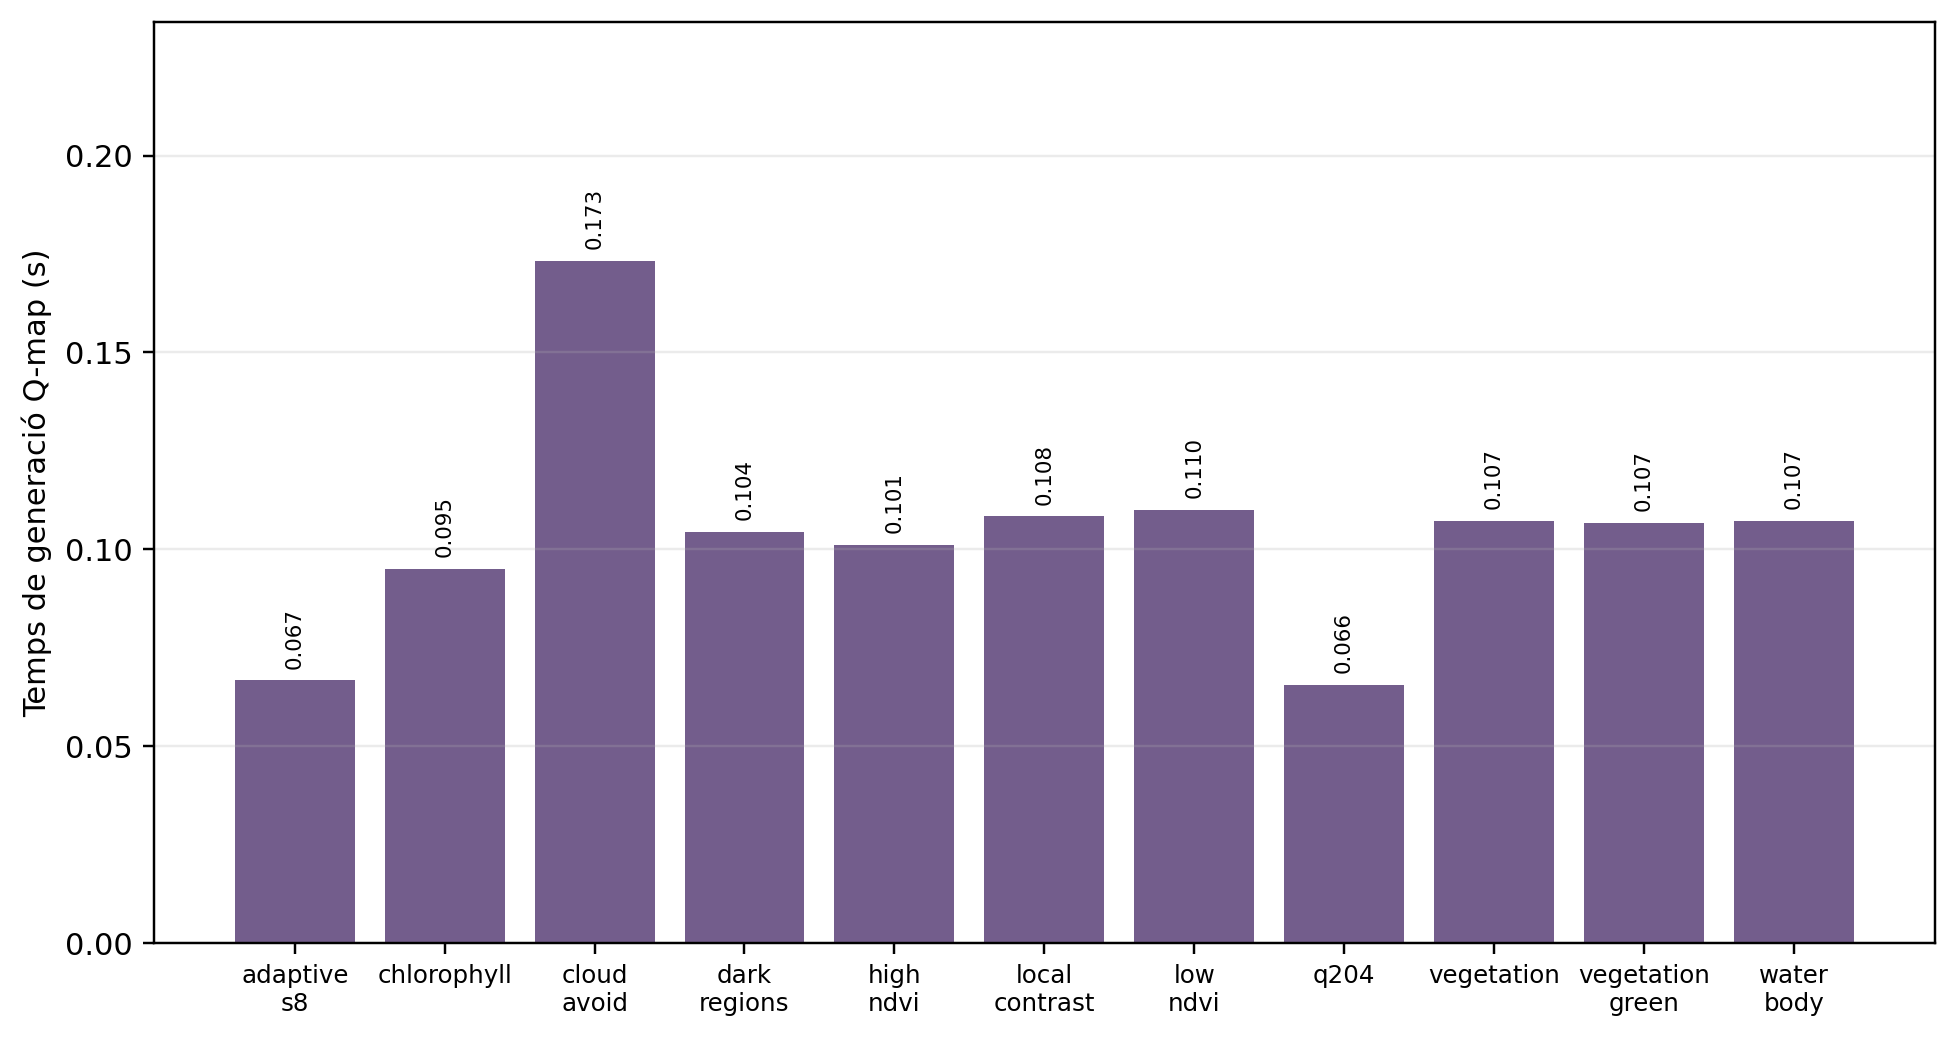
\includegraphics[width=0.88\textwidth]{raspberry_qmap_cost.png}
\caption{Temps mitjà de generació del Q-map comparat amb compressor i pipeline
complet. S'utilitza escala logarítmica perquè hi ha més de tres ordres de
magnitud de diferència.}
\label{fig:qmap_cost}
\end{figure}

Aquest resultat accepta H6 dins la mida d'entrada mesurada: el cost de decidir
la ROI automàtica és negligible davant del cost de les transformades
neuronals. No implica que qualsevol segmentador sigui gratuït. La conclusió és
específica dels presets algebraics implementats, que recorren les bandes i
calculen estadístics simples per bloc.

\section{Latència i throughput}\label{sec:throughput}

Un retall conté:

\begin{equation}
512\cdot512=262.144\;\text{posicions espacials},
\qquad
8\cdot512\cdot512=2.097.152\;\text{mostres espectrals}.
\end{equation}

Amb el compressor optimitzat, el throughput observat és:

\begin{align}
T_{espacial,enc} &= \frac{262.144}{261,32}
                   = 1.003\;\text{píxels espacials/s},\\
T_{mostres,enc} &= \frac{2.097.152}{261,32}
                   = 8.025\;\text{mostres espectrals/s}.
\end{align}

Quan s'inclou la descompressió, el temps total és 468,13~s i els valors baixen
a:

\begin{align}
T_{espacial,enc+dec} &= \frac{262.144}{468,13}
                   = 560\;\text{píxels espacials/s},\\
T_{mostres,enc+dec} &= \frac{2.097.152}{468,13}
                   = 4.480\;\text{mostres espectrals/s}.
\end{align}

La Taula~\ref{tab:throughput} evita confondre els dos escenaris.

\begin{table}[H]
\centering
\small
\begin{tabularx}{\textwidth}{lrrr>{\raggedright\arraybackslash}X}
\toprule
Ruta & Temps/retall & Píxels/s & Mostres/s & Ús principal \\
\midrule
Només compressor & 261,32~s & 1.003 & 8.025 & Codificació abans del downlink \\
Compressor+descompressor & 468,13~s & 560 & 4.480 & Càlcul d'error base o reconstrucció local \\
\bottomrule
\end{tabularx}
\caption{Throughput mesurat per un retall $8\times512\times512$. ``Píxel''
compta una posició espacial; ``mostra'' compta cada banda per separat.}
\label{tab:throughput}
\end{table}

La latència de compressió és 4~min 21~s per retall. Aquest valor és compatible
amb una demostració funcional i amb processament diferit de poques adquisicions,
però no permet afirmar per si sol processament en temps real. Una afirmació de
temps real exigiria comparar aquest throughput amb el cabal documentat del
sensor, la memòria de buffer i el cicle de servei de la missió concreta.

Com a ordre de magnitud extern, ESA descriu Sentinel-2 com una missió
multiespectral d'alt cabal que pot adquirir, emmagatzemar i descarregar fins a
1,6~TB per òrbita \cite{esa_sentinel2_operations}. Aquesta
referència no és un requisit per a aquest treball, perquè el sensor, el
maquinari i la missió són diferents, però ajuda a interpretar el resultat: una
Raspberry processant 55~MiB/h de dades crues no és una solució de temps real per
a sensors d'alt flux. En canvi, sí pot ser coherent amb processament diferit,
baixa cadència o selecció prèvia de pocs retalls. El resultat també és
consistent amb la motivació de plataformes a bord més especialitzades, com les
demostracions C3SatP/MENUT en òrbita \cite{serra2024c3satp}.

En la ruta fixed-quality amb error mesurat, el descompressor és rellevant perquè
permet obtenir la distorsió real de la passada base. En una ruta mínima de
transmissió amb el Q-map decidit sense error base, en canvi, el satèl·lit podria
executar només generació de Q-map més compressor i deixar la reconstrucció a
terra. La Taula~\ref{tab:operational_routes_cost} resumeix aquesta diferència.

\begin{table}[H]
\centering
\footnotesize
\begin{tabularx}{\textwidth}{>{\raggedright\arraybackslash}p{0.32\textwidth}r>{\raggedright\arraybackslash}X}
\toprule
Ruta & Temps & Lectura \\
\midrule
Q-map sense error base + compressió final & 261,4~s &
Cost mínim quan la qualitat local es decideix sense mesurar error base. \\
Error mesurat + Q-map + compressió final & 729,6~s &
Mesura error base, decideix qualitat i codifica el resultat final. \\
Taula precalibrada + Q-map + compressió final & 261,4~s &
Reutilitza informació calibrada a terra i evita la passada base a bord. \\
\bottomrule
\end{tabularx}
\caption{Cost per retall de tres rutes operatives sobre Raspberry. Els temps
combinen el Q-map semàntic mitjà (0,113~s) amb les mitjanes optimitzades de la
Taula~\ref{tab:rpi_optimized_time}.}
\label{tab:operational_routes_cost}
\end{table}

Els càlculs de la taula són:

\begin{equation}
0,113+261,32=261,43~\text{s},
\qquad
468,13+0,113+261,32=729,56~\text{s}.
\end{equation}

La taula precalibrada és important perquè desplaça a terra una part cara de la
decisió. No substitueix la validació de qualitat ni és universal: només és
fiable si la calibració representa bé el sensor, el tipus d'escena i les zones
que es volen protegir. Però, quan aquesta condició es compleix, pot ser una ruta
molt atractiva per a missió: manté el cost a bord pràcticament igual que una
compressió directa i evita aproximadament 468~s per retall respecte del càlcul
amb error mesurat. Per això es tracta com una opció operativa rellevant, no com
un simple detall auxiliar.

\subsection{Capacitat de servei per retalls}

Una altra manera d'interpretar la latència és com una cua de treball. Si la
Raspberry dedica un nucli de sistema i quatre fils OpenMP al compressor sense
interrupcions, la taxa màxima observada és:

\begin{equation}
\mu=\frac{3600}{261,32}=13,77\;\text{retalls/hora}.
\end{equation}

Això correspon aproximadament a 330 retalls per dia en un escenari ideal de
servei continu. Com cada RAW ocupa 4~MiB, el processador absorbiria uns
55~MiB/h de dades crues. Aquests valors són una capacitat de laboratori, no un
pressupost de missió: no inclouen adquisició, escriptura a emmagatzematge,
telemetria, altres tasques de l'OBC, períodes de baixa potència ni reinicis.

Si el sensor produeix retalls a una taxa mitjana $\lambda_a$, la cua només és
estable si:

\begin{equation}
\lambda_a<\mu.
\end{equation}

Una adquisició en ràfega podria superar temporalment $\mu$ si existeix buffer,
però el backlog hauria de buidar-se abans de la següent campanya. Aquesta
formulació és més útil que afirmar simplement que quatre minuts són molts:
permet inserir en el futur el nombre real de retalls per òrbita i comprovar si
la latència és compatible.

\subsection{Què falta per a un throughput de missió}

Per convertir la capacitat de laboratori en una conclusió de sistema calen:

\begin{itemize}[leftmargin=*]
  \item píxels o mostres generades per segon pel sensor;
  \item durada i freqüència de les adquisicions;
  \item memòria disponible per absorbir ràfegues;
  \item temps de CPU reservat per al compressor;
  \item potència mitjana i energia per retall;
  \item cabal i finestres de downlink.
\end{itemize}

Sense aquests paràmetres no es pot decidir si el 8,84\% de bitrate allibera més
recurs de sistema del que consumeix el càlcul complet. El projecte sí resol una
part concreta: el detector semàntic només representa el 0,043\% del temps de
compressió. La incertesa operativa resideix en el cost del còdec, en l'energia
per retall i en el perfil de missió.

\section{Temperatura, alimentació i repetibilitat}\label{sec:thermal}

Els registres de Raspberry indiquen valors de \code{get\_throttled} diferents
de zero, incloent \code{0xd0005} i \code{0xd0008}, i màxims de temperatura pròxims als
70~\textdegree C en algunes execucions. Això indica que les mesures es van fer
amb incidències històriques o actives d'alimentació i limitació de freqüència.
Els temps són reals de la placa utilitzada, però no representen una cota ideal
del Cortex-A53 amb alimentació estabilitzada i refrigeració controlada.

La comparació optimitzat--baseline continua sent útil perquè les dues campanyes
utilitzen la mateixa placa, el mateix nombre de fils i la mateixa càrrega.
Tanmateix, una campanya de caracterització de hardware formal hauria de fixar
governor, font d'alimentació, temperatura ambient i període de refredament, i
hauria de mesurar energia per imatge, no només temps.

\section{Cost computacional enfront d'estalvi de bits}\label{sec:cost_benefit}

La decisió final combina els Capítols~\ref{ch:resultats} i~\ref{ch:bord}. En la
mostra CSMR principal, \code{focus\_bgq128} estalvia un 8,84\% de bitrate
respecte de \code{q204}. A Raspberry, calcular el preset semàntic afegeix de
mitjana 0,113~s, un 0,043\% del temps del compressor. Per tant, dins del
pipeline actual, \textbf{sí que compensa executar el preset}. La pregunta més
difícil és si compensa la ruta completa de càlcul de qualitat amb error mesurat:
una compressió individual costa 261,32~s i compressor més descompressor costa
468,13~s per retall. Aquest cost pot ser acceptable en escenaris de baixa
cadència o processament diferit, però exigeix més optimització o hardware més
potent si es vol operar amb un flux d'adquisició alt.

Aquesta conclusió no significa que el sistema complet sigui prou ràpid. El
coll d'ampolla és el còdec neuronal C, no la selecció ROI. El treball futur
hauria de prioritzar kernels, vectorització, acceleració o un processador més
potent abans de simplificar els presets. El guany de compressió és moderat i
no justifica qualsevol cost computacional; justifica el cost concret mesurat
dels detectors algebraics.

\section{Discussió de viabilitat}\label{sec:onboard_discussion}

Els resultats permeten separar quatre nivells de viabilitat. Aquesta separació
evita barrejar una demostració funcional amb una certificació de missió:

\begin{table}[H]
\centering
\footnotesize
\begin{tabularx}{\textwidth}{>{\raggedright\arraybackslash}p{0.22\textwidth}>{\raggedright\arraybackslash}X}
\toprule
Nivell & Lectura \\
\midrule
Funcional &
Assolit: el bundle C executa compressor, descompressor i artefactes amb menys
d'1~GiB. Límit: no és software qualificat per a vol. \\
Decisió espacial &
Assolit: els presets automàtics costen 0,113~s de mitjana i no requereixen
operador. Límit: conclusió vàlida per als presets algebraics implementats. \\
Qualitat/bitrate &
Assolit dins l'abast: CSMR confirma estalvi de bitrate i ROI conservada en la
mostra seleccionada. Límit: dataset i màscares limitades. \\
Missió &
No demostrat: faltaria fixar cabal de sensor, energia, deadlines, tolerància a
fallades i hardware qualificat. \\
\bottomrule
\end{tabularx}
\caption{Lectura de viabilitat separada per nivells. Cada fila indica què queda
demostrat i quin límit impedeix convertir-ho directament en certificació de
vol.}
\label{tab:onboard_viability_levels}
\end{table}

La formulació evita dos extrems: presentar Raspberry com una certificació de
vol o descartar el resultat perquè no és el computador final. La placa serveix
per descobrir que la memòria és assumible, que quatre fils milloren el temps,
que els presets són pràcticament gratuïts i que el còdec encara necessita una
millora de throughput per a escenaris exigents.

En conjunt, H1 queda acceptada pel que fa a execució completa i memòria
limitada, H5 queda acceptada per l'acceleració amb paritat i H6 queda acceptada
pel cost negligible de la decisió espacial. La Raspberry valida aquests
criteris com a plataforma representativa de baix recurs, però no certifica el
sistema per a vol. El capítol següent resumeix aquestes respostes i delimita el
treball futur.

\thispagestyle{empty}

\cleardoublepage
% !TEX root = ../main.tex
\chapter{Conclusions i treball futur}\label{ch:conclusions}
\fancyhead[RE]{\slshape \textsf{Capítol \thechapter.\ Conclusions}}
\fancyhead[LO]{\slshape \textsf{\nouppercase \rightmark}}

\section{Resposta al problema plantejat}\label{sec:final_answer}

Aquest treball partia d'un problema operatiu: un satèl·lit no pot dependre
d'un operador que dibuixi una ROI abans de cada compressió. Alhora, aplicar
qualitat uniforme a tota la imatge desaprofita bits quan només una part és
prioritària. La solució desenvolupada combina tres elements separables:

\begin{enumerate}[leftmargin=*]
  \item un preset C identifica automàticament blocs d'interès;
	  \item una política C assigna qualitat a ROI i fons;
	  \item el compressor i el descompressor C permeten mesurar error, aplicar el
	  Q-map resultant i reconstruir la imatge sense conèixer la semàntica que l'ha
	  generat.
\end{enumerate}

La separació és la contribució de disseny principal. Permet canviar l'objectiu
de missió sense modificar el còdec: vegetació, contrast, aigua o núvols són
detectors; \code{focus} i \code{preserve-roi} són regles de qualitat. El Q-map
és el contracte entre tots dos.

El resultat quantitatiu principal és que \code{focus\_bgq128}, sobre 20 casos
CSMR seleccionats de manera reproduïble, redueix el bitrate mitjà de 4,0602 a
3,7013~bps respecte de \code{q204}. L'estalvi agregat és 8,84\%, mentre el PSNR
de la ROI augmenta de mitjana 0,203~dB i el fons disminueix 2,204~dB respecte
de \code{q204}, sempre amb la mateixa màscara ROI/fons. No s'ha obtingut massa
compressió; s'ha demostrat una
redistribució moderada, mesurable i controlada.

\begin{table}[H]
\centering
\footnotesize
\begin{tabularx}{\textwidth}{p{0.7cm}>{\raggedright\arraybackslash}X}
\toprule
 & Resposta final \\
\midrule
P1 & Sí, dins l'abast experimental: el pipeline C comprimeix, descomprimeix,
reconstrueix i conserva els artefactes necessaris amb memòria limitada. \\
P2 & Sí, amb dependència del context: els presets automàtics substitueixen la ROI
manual quan produeixen una cobertura interpretable, però no tots els presets són
útils en totes les escenes. \\
P3 & Sí, en la mostra CSMR: \code{focus\_bgq128} redueix bitrate respecte de
\code{q204} i conserva la ROI; \code{preserve-roi} canvia el compromís cap a més
fidelitat de ROI. \\
P4 & Parcialment: decidir el Q-map és molt barat, però el còdec domina el cost.
La ruta amb error mesurat és lenta; la taula precalibrada pot ser atractiva si la
calibració és representativa. \\
\bottomrule
\end{tabularx}
\caption{Resposta sintètica a les preguntes de recerca formulades al
Capítol~\ref{ch:introduccio}.}
\label{tab:research_question_answers}
\end{table}

\section{Compliment dels objectius}\label{sec:objective_answers}

Els cinc objectius definits al Capítol~\ref{ch:introduccio} s'avaluen de manera
explícita a la Taula~\ref{tab:objective_results}. La distinció entre
\emph{assolit} i \emph{assolit amb abast} evita presentar com a general un
resultat condicionat pel dataset o per la plataforma utilitzada.

\begin{table}[H]
\centering
\scriptsize
\begin{tabularx}{\textwidth}{p{0.7cm}p{2.1cm}X}
\toprule
 & Estat & Evidència de compliment \\
\midrule
O1 & Assolit amb abast & S'han integrat compressor, descompressor i format de
flux en C. Els tests i les comparacions amb la referència verifiquen el
comportament dins les toleràncies documentades. \\
O2 & Assolit amb abast & Els presets C identifiquen regions sense intervenció
manual i es combinen amb polítiques de qualitat. Alguns presets continuen
limitats per la cobertura del dataset i l'absència de bandes SWIR. \\
O3 & Assolit en la mostra & CSMR mesura bitrate real amb fitxers \code{.tfci}
i una màscara comuna. \code{focus\_bgq128} obté un 8,84\% d'estalvi mitjà
respecte de \code{q204} en els 20 casos principals. Aquesta xifra correspon al
codificador de referència, no al bitstream C sense codificació per entropia. \\
O4 & Assolit & L'optimització C aporta un speedup total mitjà
d'$1,205\times$ en 66 parelles Raspberry, sense fallades de paritat funcional. \\
O5 & Assolit amb abast & La decisió semàntica representa un 0,043\% del temps
de compressió, però calcular qualitat amb error mesurat depèn del còdec complet:
261,32~s per compressió i 468,13~s per compressió més descompressió en
Raspberry. L'estalvi de transmissió compensa el detector; la viabilitat de la
ruta completa depèn del throughput, de més optimització i de completar la
codificació per entropia o aritmètica en C. La taula precalibrada és una
alternativa prometedora quan la calibració és transferible, perquè evita la
passada d'error base. \\
\bottomrule
\end{tabularx}
\caption{Compliment dels objectius específics formulats al
Capítol~\ref{ch:introduccio}.}
\label{tab:objective_results}
\end{table}

\section{Avaluació de les hipòtesis}\label{sec:hypothesis_answers}

\begin{table}[H]
\centering
\scriptsize
\begin{tabularx}{\textwidth}{p{0.6cm}p{2.0cm}X}
\toprule
 & Estat & Resposta \\
\midrule
H1 & Acceptada amb abast & El pipeline C executa compressor i descompressor,
manté els formats i funciona en menys d'1~GiB. La correspondència amb la
referència s'ha validat amb operacions unitàries, artefactes i toleràncies; no
s'afirma identitat universal TensorFlow--C per qualsevol plataforma. \\
H2 & Parcialment acceptada & Diversos presets produeixen ROI interpretables
sense operador i mantenen qualitat en CSMR. No tots els presets funcionen en
totes les escenes i falta B11 per validar completament núvols. \\
H3 & Acceptada en la mostra & \code{focus\_bgq128} redueix bitrate real
respecte de \code{q204} i conserva la ROI en els casos seleccionats. El resultat no
es generalitza encara a qualsevol sensor o distribució. \\
H4 & Acceptada & \code{focus} afavoreix estalvi; \code{preserve-roi} fixa
Q240/Q255 a la ROI i afavoreix fidelitat. Cap política domina simultàniament
les dues dimensions. \\
H5 & Acceptada & Les optimitzacions de GDN/IGDN, depth-to-space i transformada
espectral aporten un speedup total mitjà d'1,205$\times$ amb zero fallades de
paritat en 66 parelles Raspberry. \\
H6 & Acceptada amb abast & Un preset semàntic tarda 0,113~s de mitjana: 0,043\%
del temps del compressor. El coll d'ampolla és el còdec, que també determina el
cost de calcular qualitat amb error mesurat. Amb una taula precalibrada, aquest
cost pot reduir-se, però només si la calibració representa la missió. \\
\bottomrule
\end{tabularx}
\caption{Resposta final a les hipòtesis formalitzades al
Capítol~\ref{ch:metodologia}.}
\label{tab:hypothesis_results}
\end{table}

\section{Contribucions assolides}\label{sec:contributions_final}

Les contribucions tècniques i metodològiques es poden resumir en:

\begin{itemize}[leftmargin=*]
  \item implementació C del pipeline de compressió i descompressió SORTENY,
  amb pesos exportats, format de bitstream documentat i validació d'operacions;
  \item recalibració coherent de la qualitat amb $\lambda_{max}=0,05$ i
  separació explícita de l'escala anterior;
  \item generadors C de Q-map uniforme, objectiu global, adaptatiu i semàntic;
  l'objectiu global s'ha validat com a mecanisme de conversió objectiu--Q amb
  una corba canònica, no com a estadística multiimatge;
  \item biblioteca de presets automàtics i llindars auditats, sense ROI
  manual en la ruta operativa;
  \item dues polítiques complementàries: \code{focus\_bgq128} i
  \code{preserve-roi};
  \item validació C-only de 120 retalls i validació de bitrate real amb CSMR
  mitjançant qualitat local per bloc;
  \item criteri de cribratge per proxies C-only, amb l'índex complet documentat
  com a eina auxiliar i no com a mètrica final;
  \item registre de procedència per a cada xifra utilitzada, indicant població,
  unitat i baseline;
  \item optimització incremental per Cortex-A53 i demostració Raspberry amb
  mesures de temps, RSS, temperatura i throttling;
  \item mesura separada del cost dels presets i del còdec, que permet una
  decisió cost--benefici quantitativa sobre calcular qualitat a bord.
\end{itemize}

La contribució no és un nou model neuronal entrenat. És convertir un model de
recerca en un sistema C controlable espacialment, verificable i executable en
una plataforma limitada.

\section{Recomanació operativa}\label{sec:operational_recommendation}

La configuració recomanada depèn de l'objectiu:

\begin{description}[leftmargin=3.5cm,style=nextline]
  \item[Fallback robust] \code{q204}. Qualitat uniforme, comportament fàcil
  d'auditar i cap dependència d'una detecció semàntica.
  \item[Mode principal] \code{preset + focus\_bgq128}. Adequat quan existeix
  una ROI interpretable i la missió vol reduir downlink mantenint-la.
  \item[ROI prioritària] \code{preset + preserve-roi Q240/Q128} o Q255/Q128.
  Adequat quan és preferible cedir part de l'estalvi per augmentar la garantia
  de qualitat a la regió seleccionada.
  \item[Control tècnic] \code{adaptive\_s8}. Útil per estudiar dificultat local,
  però sense estalvi de bitrate mesurable davant de \code{q204} en la mostra
  principal.
  \item[Baixa cadència o calibració coneguda] Taula precalibrada. Pot evitar la
  passada de compressor+descompressor per obtenir l'error base i estalviar uns
  468~s per retall, sempre que la calibració sigui representativa del sensor,
  escena i ROI esperats.
\end{description}

Aquesta recomanació assumeix que el preset selecciona una ROI interpretable. Si
la ROI és buida, total o massa dispersa, el Capítol~\ref{ch:resultats} mostra
que el valor operatiu baixa i que convé tornar a qualitat uniforme, canviar de
preset o revisar el llindar.

Els presets \code{cloud\_avoid}, \code{local\_contrast}, \code{vegetation},
\code{vegetation\_green} i \code{chlorophyll} disposen d'evidència principal.
\code{high\_ndvi} és un candidat útil després de l'auditoria experimental.
\code{low\_ndvi}, \code{dark\_regions} i \code{water\_body} necessiten més
cobertura. \code{clouds} i \code{cloud\_avoid} s'han de revalidar amb SWIR
abans d'atribuir-los precisió física de detecció de núvols.

\section{Limitacions}\label{sec:final_limitations}

La interpretació final està condicionada per les limitacions següents:

\begin{enumerate}[leftmargin=*]
  \item El dataset té 120 retalls de vuit bandes i no inclou B11/B12.
  \item Els 20 casos CSMR principals provenen d'un cribratge C-only; la mostra
  és deliberadament informativa i no una estimació aleatòria de tota la
  distribució.
  \item Els llindars s'han ajustat sobre el dataset disponible; encara falta
  separar conjunt de desenvolupament i conjunt de test per estimar-ne la
  transferibilitat.
  \item El bitstream C desa latents enters sense codificador per entropia o
  codificador aritmètic. El bitrate final es mesura amb CSMR \code{.tfci}.
  \item CSMR és la referència de bitrate de SORTENY amb TensorFlow Compression,
  però no substitueix la necessitat futura d'un codificador final completament
  en C.
  \item PSNR i MSE mesuren fidelitat, però no el rendiment d'una aplicació
  científica posterior.
  \item \code{global\_target} s'ha validat amb una corba canònica per mostrar el
  mecanisme i la saturació fora de rang; la seva precisió estadística requeriria
  una auditoria multiimatge i multiobjectiu.
  \item La Raspberry demostra execució de baix recurs, però les mesures estan
  afectades pels estats de throttling registrats i no representen una cota ideal
  del processador.
  \item La prova Raspberry no demostra temps real, consum energètic, tolerància
  a radiació ni qualificació espacial.
\end{enumerate}

Aquestes limitacions no invaliden la comparació interna perquè els controls
comparteixen retalls, màscares i còdec. Sí que limiten la generalització
externa.

\section{Treball futur prioritzat}\label{sec:future_work}

El següent increment hauria de prioritzar resultats de sistema, no afegir modes
sense una pregunta experimental clara.

\subsection{Codificació per entropia o aritmètica en C}

La prioritat és integrar un codificador per entropia o aritmètic compatible amb
els latents. Això permetria eliminar la dependència de CSMR per mesurar bitrate
real, comparar temps completament en C i estudiar el cost del codificador a
bord. El format hauria d'incloure versió, longituds, comprovació d'integritat i
límits estrictes abans de modificar la ruta operativa validada.

\subsection{Validació espectral i de dataset}

Cal repetir els presets de núvol amb B11 i ampliar estacions, cobertes i
sensors. Els llindars s'haurien d'estimar sobre un conjunt de desenvolupament
i avaluar sobre un conjunt separat. \code{water\_body} necessita específicament
un full complet a llindar 0,10; un únic crop CSMR no permet generalitzar.

\subsection{Mètriques orientades a tasca}

La ROI hauria d'avaluar-se també amb una tasca final: classificació de coberta,
segmentació, detecció d'incendis, estimació de clorofil·la o una altra variable
de missió. Una variació petita de PSNR pot ser irrellevant o crítica segons la
tasca.

\subsection{Rendiment i energia}

El throughput del Cortex-A53 és insuficient per afirmar processament en temps
real d'un sensor d'alta taxa. Cal perfilar convolucions, explorar NEON efectiu,
tiling, acceleradors o un OBC més potent, i mesurar joules per retall. La
comparació futura ha d'utilitzar el cabal del sensor i el calendari de
contactes de la missió concreta. També cal decidir formalment quan convé usar
error mesurat i quan convé usar una taula precalibrada: la decisió depèn de la
cadència, energia disponible, memòria de buffer i risc de transferir una
calibració fora del seu domini.

\subsection{Qualitat multidimensional}

Lambdes independents per bandes espectrals o grups de canals latents podrien
adaptar millor el pressupost a una tasca. Les lambdes per capes internes són una
línia més profunda: canvien la funció del model i probablement exigeixen
redisseny i reentrenament. No s'han de presentar com una extensió directa del
Q-map actual.

\section{Conclusió final}\label{sec:final_conclusion}

El treball demostra que és possible controlar espacialment un compressor
neuronal multiespectral des de C amb una interfície simple i reproduïble. La
selecció automàtica elimina la necessitat d'una ROI dibuixada per un operador,
i el cost de fer-la és negligible davant del còdec. En casos representatius,
la política focus redueix aproximadament un 8,84\% el bitrate real respecte de
qualitat uniforme, conservant la regió seleccionada i traslladant la distorsió
al fons. Preserve-roi ofereix una alternativa quan la fidelitat de la ROI té
més valor que l'estalvi màxim.

La implementació optimitzada funciona en Raspberry amb memòria limitada i és
un $1,205\times$ més ràpida en speedup total mitjà que la versió baseline, cosa
que equival a reduir el temps aproximadament un 17\%, sense canvis funcionals
detectats. La mateixa prova mostra el límit actual: la
latència del còdec continua sent de minuts per retall quan es calcula qualitat
amb error mesurat. La taula precalibrada obre una ruta més lleugera si la missió
pot assumir una calibració prèvia representativa, però no elimina la necessitat
de validar qualitat i transferibilitat. Per tant, la conclusió és positiva però
acotada: el control espacial és útil i barat; la prioritat per apropar el
sistema a una missió real és augmentar el throughput, completar la codificació
per entropia o aritmètica en C i decidir quan és acceptable substituir error
mesurat per calibració precalculada.

\thispagestyle{empty}

\appendix
\cleardoublepage
% !TEX root = ../main.tex
\chapter{Reproduïbilitat i comandes}\label{app:reproducibility}
\fancyhead[RE]{\slshape \textsf{Apèndix \thechapter.\ Reproduïbilitat}}
\fancyhead[LO]{\slshape \textsf{\nouppercase \rightmark}}

Aquest apèndix descriu una ruta de reproducció gradual. Primer s'identifica el
repositori, l'estructura mínima, les dependències i el format de dades. Després
s'executa una prova curta que compila el codi C i processa una imatge amb la
ruta mesurada \(\lambda/Q\). Les campanyes completes de CSMR i Raspberry es
presenten al final com a reproducció avançada perquè requereixen dependències,
checkpoints o hardware específics.

\section{Repositori públic}

El repositori públic del projecte és:

\begin{center}
\url{https://github.com/Crist407/Implementacio-compressor-basat-en-xarxes-neurals-per-a-us-en-satel-lit}
\end{center}

El repositori conté el codi, pesos, configuració, dataset RAW públic i fonts de
la memòria. Els checkpoints complets, bundles Raspberry i entorns locals no
formen part de Git perquè són artefactes generats. El fitxer
\code{PUBLIC\_ARTIFACTS.md} resumeix quins elements són públics i quins es
regeneren amb scripts.

\section{Estructura pública del repositori}

\begin{table}[H]
\centering
\small
\begin{tabularx}{\textwidth}{lX}
\toprule
Directori & Contingut \\
\midrule
\code{src/c/} & Implementació C del compressor, descompressor, capes i
generadors de Q-map. \\
\code{src/python/analysis/} & Orquestradors i scripts d'anàlisi, inclosa la
ruta mesurada \(\lambda/Q\). \\
\code{src/python/reference/} & Referència Python/TensorFlow de SORTENY. \\
\code{scripts/raspberry/} & Benchmarks autocontinguts per Raspberry. \\
\code{scripts/docs/} & Generació de figures i compilació compatible de la
memòria. \\
\code{config/} & Llindars, calibració mínima \code{lambda005} i configuracions
de presets. \\
\code{weights/} & Pesos exportats del model necessaris per a la ruta C. \\
\code{data/} & Dataset RAW de 120 retalls, mostra mínima i instruccions de
visualització. \\
\code{docs/informe\_final/} & Fonts \LaTeX, figures i bibliografia de la
memòria. \\
\bottomrule
\end{tabularx}
\caption{Estructura del repositori públic utilitzada per reproduir els exemples
d'aquest apèndix.}
\label{tab:public_repo_structure}
\end{table}

\section{Instal·lació mínima}

La prova bàsica requereix un compilador C, \code{make}, Python 3 i NumPy. La
ruta CSMR necessita TensorFlow i TensorFlow Compression, però no són necessaris
per a la prova inicial.

\begin{verbatim}
python3 -m venv .venv
source .venv/bin/activate
pip install -r requirements.txt
\end{verbatim}

El repositori inclou una mostra RAW, el dataset de 120 retalls i la calibració
necessària per executar la ruta pública:

\begin{verbatim}
data/T31TCG_20230907T104629_5.8_512_512_2_1_0.raw
data/Sentinel2A_crop_test/
config/fq_calibration_lambda005.tsv
\end{verbatim}

\section{Dataset i visualització RAW}

Cada RAW té $8\times512\times512$ valors \code{uint16}, és a dir,
4.194.304 bytes. Els fitxers no tenen capçalera i estan guardats en ordre BSQ.
Per obrir-los amb Fiji/ImageJ cal utilitzar \code{File -> Import -> Raw...} i
configurar:

\begin{itemize}[leftmargin=*]
  \item tipus d'imatge: \code{16-bit Unsigned};
  \item amplada i alçada: $512\times512$;
  \item nombre d'imatges: 8;
  \item offset i separació entre imatges: 0;
  \item ordre de bytes: little-endian.
\end{itemize}

Per inspecció visual en color natural aproximat, les bandes recomanades són B04
com a vermell, B03 com a verd i B02 com a blau. El fitxer \code{data/README.md}
resumeix el format i els passos de visualització.

També es pot generar un paquet de quicklook sense executar el còdec:

\begin{verbatim}
python3 src/python/utils/manual_roi_quicklook.py \
  --input data/T31TCG_20230907T104629_5.8_512_512_2_1_0.raw \
  --output-dir output/checkpoints/quicklook_example \
  --pattern empty \
  --skip-qmap
\end{verbatim}

\section{Compilació C}

La compilació de la ruta C principal és:

\begin{verbatim}
make MODE=release OMP=1
make MODE=release OMP=1 test_ops
\end{verbatim}

Els binaris utilitzats per les proves d'aquest apèndix són:
\code{sorteny\_compressor}, \code{sorteny\_decompressor},
\code{sorteny\_fq\_qmap} i \code{sorteny\_semantic\_qmap}. El test
\code{test\_ops} comprova operadors interns del decoder abans d'executar una
campanya completa.

\section{Reproducció ràpida}

Després d'instal·lar dependències i compilar el C, la prova mínima processa una
imatge amb el mode \code{focus\_bgq128\_measured}:

\begin{verbatim}
python3 src/python/analysis/run_lambda005_measured_quality_route.py \
  --output-dir output/checkpoints/quickstart_measured_route \
  --modes focus_bgq128_measured \
  --threads 4
\end{verbatim}

Una execució correcta crea el directori
\code{output/checkpoints/quickstart\_measured\_route}. Aquesta prova valida el
camí essencial: entrada RAW, còdec C, error base, càlcul de qualitat local,
Q-map i reconstrucció final.

\section{Comprovació de sortides}

La prova ràpida ha de generar:

\begin{itemize}[leftmargin=*]
  \item Q-maps de 1.024 bytes;
  \item bitstreams C llegibles pel descompressor;
  \item reconstruccions RAW de 4.194.304 bytes;
  \item \code{metrics.csv}, \code{metrics.json} i \code{run\_meta.json}.
\end{itemize}

Les invariants principals es comproven amb:

\begin{verbatim}
CHECKPOINT=output/checkpoints/quickstart_measured_route

find "$CHECKPOINT/qmaps" -name '*.raw' -printf '%p %s\n'
find "$CHECKPOINT/reconstructions" -name '*.raw' -printf '%p %s\n'
sed -n '1,20p' "$CHECKPOINT/metrics.csv"
\end{verbatim}

\section{Comprovació dels extractes públics}

Les xifres principals de la memòria també es poden inspeccionar sense regenerar
els checkpoints complets. El directori \code{docs/informe\_final/evidence/}
conté extractes CSV petits amb els resums que alimenten el registre
d'evidències de l'Apèndix~\ref{app:evidence}.

\begin{verbatim}
ls docs/informe_final/evidence
sed -n '1,10p' docs/informe_final/evidence/csmr_policy_summary.csv
sed -n '1,10p' docs/informe_final/evidence/q204_same_mask_summary.csv
sed -n '1,10p' docs/informe_final/evidence/raspberry_operational_costs.csv
\end{verbatim}

El càlcul següent comprova tres valors destacats del cos principal: l'estalvi de
\code{focus\_bgq128} contra \code{q204}, el cost de la ruta amb error mesurat i
el cost relatiu de generar un Q-map semàntic.

\begin{verbatim}
python3 - <<'PY'
import csv

with open("docs/informe_final/evidence/csmr_policy_summary.csv",
          newline="") as f:
    rows = {r["policy"]: r for r in csv.DictReader(f)}
q204 = float(rows["q204"]["tfci_bps_mean"])
focus = float(rows["focus_bgq128"]["tfci_bps_mean"])
print("estalvi_focus_vs_q204_pct =", 100 * (1 - focus / q204))

with open("docs/informe_final/evidence/raspberry_operational_costs.csv",
          newline="") as f:
    costs = {r["metric"]: float(r["value"]) for r in csv.DictReader(f)}
print("ruta_error_mesurat_s =", costs["measured_error_route"])

with open("docs/informe_final/evidence/qmap_cost_by_type.csv",
          newline="") as f:
    qmap = {r["command_type"]: r for r in csv.DictReader(f)}
print("qmap_semantic_pct_compress =",
      qmap["semantic"]["qmap_pct_of_compress_mean"])
PY
\end{verbatim}

Aquesta comprovació valida les xifres agregades publicades. La regeneració de
tota una campanya continua requerint les rutes avançades de CSMR o Raspberry
descrites més avall.

\section{Ruta mesurada \texorpdfstring{$\lambda/Q$}{lambda/Q}}

La ruta mesurada implementa la cadena:

\begin{center}
\fbox{\begin{minipage}{0.92\textwidth}
\centering
compressió/descompressió base $\rightarrow$ error base $\rightarrow$
fórmules fixed-quality $\rightarrow$ $\lambda/Q$ $\rightarrow$ Q-map
$\rightarrow$ compressió final $\rightarrow$ mètriques
\end{minipage}}
\end{center}

Per executar una prova amb dos modes:

\begin{verbatim}
OUT=output/checkpoints/lambda005_measured_quality_route_smoke

python3 src/python/analysis/run_lambda005_measured_quality_route.py \
  --output-dir "$OUT" \
  --modes global_target_measured focus_bgq128_measured \
  --threads 4
\end{verbatim}

Per executar tots els modes implementats per defecte:

\begin{verbatim}
OUT=output/checkpoints/lambda005_measured_quality_route_full

python3 src/python/analysis/run_lambda005_measured_quality_route.py \
  --output-dir "$OUT" --threads 4
\end{verbatim}

Els modes suportats són \code{global\_target\_measured},
\code{adaptive\_s8\_measured}, \code{focus\_bgq128\_measured},
\code{target\_focus\_bgq128\_measured},
\code{preserve\_roi\_q240\_bgq128} i
\code{preserve\_roi\_q255\_bgq128}. Els detalls de configuració de cada mode es
descriuen a l'Apèndix~\ref{app:config}.

\section{Ruta precalibrada}

La ruta precalibrada utilitza informació obtinguda fora de la placa per generar
Q-maps sense repetir la passada base de compressor/descompressor. És útil per
proves ràpides, comparatives i escenaris en què la calibració sigui
representativa.

Q-map uniforme:

\begin{verbatim}
CAL=config/fq_calibration_lambda005.tsv

./sorteny_fq_qmap \
  --calibration "$CAL" \
  --target-from-q 204 \
  --output-qmap output/checkpoints/q204.raw
\end{verbatim}

Q-map semàntic amb preset i política:

\begin{verbatim}
CAL=config/fq_calibration_lambda005.tsv
IN=data/T31TCG_20230907T104629_5.8_512_512_2_1_0.raw

./sorteny_semantic_qmap \
  --input "$IN" \
  --bands 8 --height 512 --width 512 \
  --band-layout sentinel2-8 --preset cloud_avoid --threshold 0.50 \
  --semantic-policy focus --foreground-boost 16 --background-q 128 \
  --calibration "$CAL" \
  --output-qmap output/checkpoints/cloud_avoid_focus_bgq128.raw \
  --summary-tsv output/checkpoints/cloud_avoid_focus_bgq128.tsv
\end{verbatim}

\section{Reproducció avançada: CSMR i bitrate real}

El bitrate real de SORTENY es mesura amb la ruta Python/TensorFlow Compression
del model. Els auditors CSMR converteixen cada Q-map en un array de
$\lambda=Q\cdot0,05/255$ i executen la referència amb \code{quality\_array}.
Aquestes campanyes requereixen dependències Python addicionals i els
checkpoints de selecció corresponents.

\begin{verbatim}
SEL=output/checkpoints/20260620_lambda005_full_csmr_case_selection
OUT=output/checkpoints/20260623_lambda005_csmr_selected_cases_bitrate_final

python3 src/python/analysis/audit_csmr_selected_cases_from_full.py \
  --selection-checkpoint "$SEL" \
  --lambda-max 0.05 --output-dir "$OUT"
\end{verbatim}

\begin{verbatim}
THR=output/checkpoints/20260625_lambda005_threshold_optimization
OUT=output/checkpoints/20260626_lambda005_csmr_experimental_threshold_modes

python3 src/python/analysis/audit_csmr_experimental_threshold_modes.py \
  --threshold-checkpoint "$THR" \
  --lambda-max 0.05 --output-dir "$OUT"
\end{verbatim}

\begin{verbatim}
OUT=output/checkpoints/20260627_lambda005_csmr_preserve_roi_policy

python3 src/python/analysis/audit_csmr_preserve_roi_policy.py \
  --lambda-max 0.05 --output-dir "$OUT"
\end{verbatim}

Aquestes proves són més costoses que la ruta C-only i depenen de l'entorn
Python/TensorFlow. Per això el cos de la memòria separa clarament proxies C de
bitrate real \code{.tfci}.

\section{Reproducció avançada: Raspberry}

Els benchmarks Raspberry requereixen una placa configurada i els bundles
autocontinguts generats per al projecte. La prova del còdec optimitzat és:

\begin{verbatim}
nohup env INCLUDE_EXPERIMENTAL=1 THREADS_LIST="4" \
  scripts/raspberry/run_lambda005_bundle_benchmark.sh \
  > rpi_optimized_lambda005_t4.log 2>&1 &
\end{verbatim}

El cost de generar Q-maps sense executar el còdec s'aïlla amb:

\begin{verbatim}
nohup env INCLUDE_EXPERIMENTAL=1 REPEATS=3 \
  scripts/raspberry/run_lambda005_qmap_cost_benchmark.sh \
  > rpi_qmap_cost_lambda005.log 2>&1 &
\end{verbatim}

La integritat mínima d'un checkpoint Raspberry es comprova amb:

\begin{verbatim}
find "$CHECKPOINT" -name DONE | wc -l
find "$CHECKPOINT" -name run_meta.tsv | wc -l
find "$CHECKPOINT" -name '*.time.txt' | wc -l
find "$CHECKPOINT" -name qmap.raw -size 1024c | wc -l
tar -tzf "${CHECKPOINT}.tar.gz" >/dev/null
sha256sum "${CHECKPOINT}.tar.gz"
\end{verbatim}

\section{Figures i compilació de la memòria}

Les figures derivades del cos principal es regeneren amb:

\begin{verbatim}
python3 scripts/docs/build_final_report_figures.py
\end{verbatim}

La memòria es compila amb el flux compatible, sense modificar la plantilla
institucional original:

\begin{verbatim}
scripts/docs/build_informe_final_compat.sh
\end{verbatim}

Una compilació correcta no ha de deixar cites, referències ni figures sense
resoldre.

\section{Verificacions locals finals}

Abans de considerar una reproducció local com a vàlida, s'han d'executar com a
mínim:

\begin{verbatim}
SCRIPT=src/python/analysis/run_lambda005_measured_quality_route.py
python3 -m py_compile "$SCRIPT"
make MODE=release OMP=1
make MODE=release OMP=1 test_ops
git diff --check
\end{verbatim}

Les campanyes completes generen més artefactes que els inclosos a Git. La seva
procedència, mida, hash i relació amb les taules i figures del cos principal es
documenten a l'Apèndix~\ref{app:evidence}.

\cleardoublepage
% !TEX root = ../main.tex
\chapter{Configuració de modes i presets}\label{app:configuration}\label{app:config}
\fancyhead[RE]{\slshape \textsf{Apèndix \thechapter.\ Configuració}}
\fancyhead[LO]{\slshape \textsf{\nouppercase \rightmark}}

Aquest apèndix és una fitxa de configuració. Serveix per consultar els valors
exactes que connecten la memòria amb el repositori públic: escala de Q, modes de
qualitat, presets automàtics, llindars, etiquetes de cobertura ROI i variants
auxiliars del codi. No és una secció de resultats ni una repetició del disseny:
el Capítol~\ref{ch:control} explica per què es defineixen aquests modes, el
Capítol~\ref{ch:metodologia} explica com s'avaluen i el
Capítol~\ref{ch:resultats} presenta les mesures obtingudes.

Les comandes de reproducció no es repeteixen aquí: són a
l'Apèndix~\ref{app:reproducibility}. Aquest apèndix conté només els paràmetres
que aquelles comandes consumeixen o generen. El registre de procedència de les
xifres queda reservat a l'Apèndix~\ref{app:evidence}.

\section{Escala Q/lambda}

La configuració principal utilitza l'escala \code{lambda005}, on el valor Q de
8 bits es converteix a lambda mitjançant:

\begin{equation}
\lambda(Q)=\frac{Q}{255}\cdot0,05.
\label{eq:app_q_lambda}
\end{equation}

\begin{table}[H]
\centering
\small
\begin{tabularx}{\textwidth}{r r X}
\toprule
Q & $\lambda$ & Lectura dins la configuració \\
\midrule
64 & 0,01255 & Valor de fons molt agressiu, reservat a proves de Q baixa. \\
96 & 0,01882 & Valor de fons agressiu, també fora de la configuració principal. \\
128 & 0,02510 & Mínim utilitzat per al fons en la ruta principal. \\
204 & 0,04000 & Referència uniforme històrica i baseline principal. \\
240 & 0,04706 & Valor alt per preservar ROI en configuracions de dos nivells. \\
255 & 0,05000 & Valor màxim representable en l'escala actual. \\
\bottomrule
\end{tabularx}
\caption{Valors representatius de Q i lambda en l'escala \code{lambda005}.}
\label{tab:q_lambda_appendix}
\end{table}

El format \code{uint8} permet Q entre 0 i 255. En aquesta memòria, la ruta
principal utilitza Q128--Q255 perquè és la zona amb més cobertura de validació.
Els valors Q$<128$ no són invàlids: simplement impliquen una degradació més
agressiva i es tracten com una línia experimental que requereix validació
específica.

\section{Modes principals}

Els modes de la Taula~\ref{tab:app_main_modes} són els noms que apareixen a la
memòria i a les rutes de reproducció. La taula fixa la regla de Q; la
interpretació experimental es dona al cos principal.

\begingroup
\scriptsize
\setlength{\tabcolsep}{2pt}
\begin{longtable}{p{2.3cm}p{2.5cm}p{5.4cm}p{2.1cm}}
\caption{Modes principals de Q-map documentats a la memòria.}\label{tab:app_main_modes}\\
\toprule
Mode & Entrada de decisió & Regla de Q & Ús de reproducció \\
\midrule
\endfirsthead
\toprule
Mode & Entrada de decisió & Regla de Q & Ús de reproducció \\
\midrule
\endhead
\code{q204} & Q explícita & Tots els blocs reben Q=204. No usa ROI ni target.
& Q-map base i comparació uniforme. \\
\code{global\_target} & MSE o PSNR objectiu & La calibració calcula un únic
$Q^\star$ i tots els blocs reben aquest valor. & Ruta mesurada global. \\
\code{adaptive\_s8} & Error relatiu per bloc & Cada bloc rep
$Q_i=\operatorname{clip}(204+8z_i)$, amb mitjana propera a 204. & Ruta
mesurada adaptativa. \\
\code{focus\_bgq128} & Preset + base adaptativa & ROI:
$\operatorname{clip}(Q_{\mathrm{adaptive},i}+16)$; fons: Q128. & Ruta amb
preset i fons Q128. \\
\code{preserve-roi} & Preset + Q fixa ROI/fons & ROI: Q240 o Q255; fons: Q128.
No usa base adaptativa dins la ROI. & Rutes preserve Q240/Q255. \\
\bottomrule
\end{longtable}
\endgroup

\section{Modes auxiliars}

Hi ha variants implementades que ajuden a reproduir campanyes de cribratge, però
no són les rutes principals de lectura de la memòria:

\begin{table}[H]
\centering
\small
\begin{tabularx}{\textwidth}{p{3.0cm}X}
\toprule
Variant & Ús de reproducció \\
\midrule
\code{boost-only} & Manté la base adaptativa al fons i incrementa Q només a la
ROI. Variant disponible al generador semàntic. \\
\code{focus\_bgpen24} & Configuració auxiliar del full C-only: reforça ROI i
redueix el fons respecte de la base adaptativa, sense imposar Q128. \\
\code{target-focus} & Variant que calcula Q dins la ROI a partir d'un objectiu
de MSE o PSNR; correspon a la ruta \code{target\_focus\_bgq128\_measured} quan
el fons es fixa a Q128. \\
\bottomrule
\end{tabularx}
\caption{Modes auxiliars documentats per traçabilitat. No substitueixen els
modes principals de la Taula~\ref{tab:app_main_modes}.}
\label{tab:app_aux_modes}
\end{table}

Les tres variants comparteixen notació. Sigui $m_i$ la màscara generada pel
preset, amb $m_i=1$ dins la ROI i $m_i=0$ al fons. Sigui
$Q_{\mathrm{adaptive},i}$ la base adaptativa del bloc. La funció
$\operatorname{clip}(\cdot)$ limita el resultat al rang de Q permès.

\paragraph{\code{boost-only}.}
Aquesta variant només modifica la ROI. El fons queda igual que a la base
adaptativa:

\begin{equation}
Q_i^{boost}=
\begin{cases}
\operatorname{clip}(Q_{\mathrm{adaptive},i}+b), & m_i=1,\\
Q_{\mathrm{adaptive},i}, & m_i=0.
\end{cases}
\end{equation}

El paràmetre $b$ és el reforç de primer pla. Aquesta política és útil per
executar una variant en què només canvien els blocs marcats com a ROI.

\paragraph{\code{focus\_bgpen24}.}
Aquesta configuració combina reforç de ROI i penalització relativa del fons:

\begin{equation}
Q_i^{bgpen24}=
\begin{cases}
\operatorname{clip}(Q_{\mathrm{adaptive},i}+16), & m_i=1,\\
\operatorname{clip}(Q_{\mathrm{adaptive},i}-24), & m_i=0.
\end{cases}
\end{equation}

A diferència de \code{focus\_bgq128}, el fons no queda fixat a Q128. Cada bloc
de fons conserva la seva variació adaptativa, però amb una penalització de 24
unitats de Q.

\paragraph{\code{target-focus}.}
Aquesta variant substitueix el reforç fix de la ROI per una decisió basada en
un objectiu de qualitat. Dins la ROI, el valor $Q_{\mathrm{target}}$ es calcula
a partir d'un MSE o PSNR objectiu mitjançant la calibració fixed-quality. El
fons pot quedar fixat o penalitzat segons la configuració concreta:

\begin{equation}
Q_i^{target}=
\begin{cases}
Q_{\mathrm{target}}, & m_i=1,\\
Q_{\mathrm{fons}}, & m_i=0\ \text{si es fixa un fons},\\
\operatorname{clip}(Q_{\mathrm{adaptive},i}-p), & m_i=0\ \text{si es penalitza}.
\end{cases}
\end{equation}

La utilitat d'aquest mode és provar una ROI guiada directament per un objectiu
de qualitat, en lloc d'un reforç constant.

\section{Presets automàtics}

Els presets transformen una magnitud derivada de la imatge en una màscara ROI.
La Taula~\ref{tab:app_presets} és una taula de consulta de la configuració
pública. Els valors coincideixen amb \code{config/auto\_thresholds\_lambda005.tsv}
quan el preset forma part de la configuració ajustada. El preset \code{clouds}
també apareix al full C-only com a complement de \code{cloud\_avoid}; es
documenta aquí per coherència amb el disseny factorial.

\begingroup
\scriptsize
\setlength{\tabcolsep}{2pt}
\begin{longtable}{p{2.6cm}p{3.1cm}p{1.7cm}p{6.5cm}}
\caption{Presets automàtics i llindars de la configuració \code{lambda005}.}
\label{tab:app_presets}\\
\toprule
Preset & Magnitud i bandes & Condició & Lectura i limitació principal \\
\midrule
\endfirsthead
\toprule
Preset & Magnitud i bandes & Condició & Lectura i limitació principal \\
\midrule
\endhead
\code{cloud\_avoid} & Fracció CBY baixa, B02/B03/B04 & $\leq0,50$ &
Família núvol/no-núvol. Sense B11/SWIR és un fallback visible, no una detecció
completa de núvols. \\
\code{clouds} & Fracció CBY alta, B02/B03/B04 & $\geq0,50$ & Complement de
\code{cloud\_avoid}; comparteix la limitació de no disposar de B11/SWIR. \\
\code{local\_contrast} & Desviació visible, B02/B03/B04 & $\geq0,035$ &
Textura visible. No representa una classe física; selecciona variació local. \\
\code{high\_ndvi} & NDVI, B08/B04 & $\geq0,50$ & Vegetació amb criteri més
restrictiu que \code{vegetation}. \\
\code{vegetation} & NDVI, B08/B04 & $\geq0,40$ & Vegetació amb llindar empíric
del dataset. \\
\code{vegetation\_green} & GNDVI, B08/B03 & $\geq0,50$ & Vegetació amb banda
verda; la lectura no és idèntica a NDVI. \\
\code{chlorophyll} & NDCI, B05/B04 & $\geq0,10$ & Proxy de clorofil·la; la
interpretació física és limitada sense més context biofísic. \\
\code{low\_ndvi} & NDVI, B08/B04 & $\leq0,15$ & NDVI baix; pot agrupar sòl,
cobertes no vegetades, ombres, aigua o valors negatius. \\
\code{dark\_regions} & Mitjana visible, B02/B03/B04 & $\leq0,26$ & Brillantor
visible baixa; pot generar ROI àmplies si l'escena és globalment fosca. \\
\code{water\_body} & NDWI, B03/B08 & $\geq0,10$ & Candidat d'aigua simple, no
una classificació hidrològica completa. \\
\bottomrule
\end{longtable}
\endgroup

Els índexs normalitzats utilitzen la forma:

\begin{equation}
I(A,B)=\frac{A-B}{A+B+\epsilon},
\end{equation}

on $\epsilon$ evita divisions per zero. Les correspondències són: NDVI amb B08 i
B04; GNDVI amb B08 i B03; NDCI amb B05 i B04; NDWI amb B03 i B08. Els llindars
són paràmetres de configuració del projecte, no constants universals de
teledetecció \cite{rouse1974ndvi,gitelson1996gndvi,mishra2012ndci,mcfeeters1996ndwi}.

\section{Cobertura ROI}

La cobertura ROI és el percentatge de blocs marcats pel preset:

\begin{equation}
C=100\frac{\sum_i m_i}{1024}.
\end{equation}

\begin{table}[H]
\centering
\small
\begin{tabularx}{\textwidth}{p{2.5cm}p{3.2cm}X}
\toprule
Etiqueta & Rang de cobertura & Ús interpretatiu \\
\midrule
\code{no\_roi} & $C=0$ & Cap bloc rep tractament de ROI. \\
\code{low\_roi} & $0<C<10\%$ & ROI petita; pot ser sensible al veïnat de blocs de fons. \\
\code{mid\_roi} & $10\%\leq C\leq70\%$ & Cobertura intermèdia, útil per comparar ROI i fons. \\
\code{high\_roi} & $70\%<C<100\%$ & ROI ampla; queda poc fons per assumir degradació. \\
\code{all\_roi} & $C=100\%$ & Tota la imatge és ROI i desapareix la redistribució ROI/fons. \\
\bottomrule
\end{tabularx}
\caption{Etiquetes de cobertura utilitzades en l'anàlisi. No són presets i no
modifiquen el Q-map.}
\label{tab:app_roi_coverage}
\end{table}

Aquestes etiquetes només classifiquen casos després de calcular la màscara. No
canvien cap llindar ni cap valor Q. Són útils per detectar situacions en què una
política espacial pot perdre sentit: ROI buida, ROI total o ROI massa dispersa.

\section{Correspondència amb fitxers públics}

\begin{table}[H]
\centering
\small
\begin{tabularx}{\textwidth}{p{3.0cm}p{4.1cm}X}
\toprule
Element & Fitxer públic & Relació amb la reproducció \\
\midrule
Llindars de presets & \path{config/auto_thresholds_lambda005.tsv} &
Llegeix els llindars que fan servir les rutes amb presets automàtics. \\
Calibració Q/lambda & \path{config/fq_calibration_lambda005.tsv} &
Proporciona l'escala i coeficients necessaris per convertir objectius de
qualitat en Q. \\
Dataset RAW & \path{data/Sentinel2A_crop_test/} & Proporciona els retalls
multiespectrals per executar exemples públics. \\
Guia de reproducció & \path{docs/informe_final/AppendixA/text_app_a.tex} &
Conté les comandes; aquest apèndix només n'especifica els paràmetres. \\
\bottomrule
\end{tabularx}
\caption{Fitxers públics que materialitzen la configuració descrita en aquest
apèndix.}
\label{tab:app_public_config_files}
\end{table}

Aquests fitxers permeten reproduir la ruta pública descrita a
l'Apèndix~\ref{app:reproducibility}. Si es canvien pesos, bandes, normalització
o escala de lambda, aquests fitxers també s'han de revisar perquè el Q-map
continuï representant la qualitat prevista.

\cleardoublepage
% !TEX root = ../main.tex
\chapter{Registre d'evidències}\label{app:evidence}
\fancyhead[RE]{\slshape \textsf{Apèndix \thechapter.\ Evidències}}
\fancyhead[LO]{\slshape \textsf{\nouppercase \rightmark}}

\section*{Pendent de fer}
\iffalse

\section{Objectiu del registre}

Cada afirmació quantitativa de la memòria s'associa a una població, una unitat,
un baseline i un checkpoint. El fitxer font llegible per màquina és
\code{docs/informe\_final/evidence\_registry.csv}. Aquest apèndix en presenta la
versió editorial.

La traçabilitat evita tres errors:

\begin{itemize}[leftmargin=*]
  \item barrejar proxies C-only amb bitrate real CSMR;
  \item comparar mitjanes obtingudes sobre poblacions diferents sense indicar
  el nombre de casos;
  \item reutilitzar una xifra de l'escala $\lambda_{max}=0,125$ com si fos de
  la calibració actual $\lambda_{max}=0,05$.
\end{itemize}

\section{Checkpoints principals}

\begin{longtable}{p{4.2cm}p{9.8cm}}
\caption{Procedència dels blocs d'evidència principals.}\label{tab:checkpoints}\\
\toprule
Checkpoint & Contingut utilitzat \\
\midrule
\endfirsthead
\toprule
Checkpoint & Contingut utilitzat \\
\midrule
\endhead
\path{20260613_lambda005_recalibration_audit} &
Calibracions Q--MSE i Q--PSNR per a $\lambda_{max}=0,05$, incloent la corba
canonical utilitzada per \code{global\_target}. \\
\path{20260619_lambda005_semantic_presets_full_auto_modes} &
Full C-only de 120 retalls, 10 presets i 4 polítiques; resultats per bloc,
resums i proxies latents. \\
\path{20260622_lambda005_full_analysis_report} &
Anàlisi derivada del full, casos bons, límit i candidats CSMR. \\
\path{20260623_lambda005_csmr_selected_cases_bitrate_final} &
CSMR principal: 20 retalls i 60 subcasos amb Q204, adaptive-s8 i focus. \\
\path{20260624_lambda005_final_evidence_pack} &
Resums consolidats de bitrate, PSNR i deltes respecte dels controls. \\
\path{20260625_lambda005_threshold_optimization} &
Barratge C-only de thresholds automàtics. \\
\path{20260626_lambda005_csmr_experimental_threshold_modes} &
CSMR de high-NDVI, low-NDVI, dark-regions i water-body. \\
\path{20260627_lambda005_preserve_roi_policy_audit} &
Auditoria C-only de preserve-roi Q240/Q128 i Q255/Q128. \\
\path{20260628_lambda005_csmr_preserve_roi_policy} &
Bitrate CSMR i qualitat de preserve-roi. \\
\path{20260631_lambda005_report_reframed_evidence} &
Reanàlisi amb Q204 com a baseline i una mateixa màscara per ROI/fons. \\
\path{20260613_raspberry_lambda005_benchmark_report} &
Baseline Raspberry amb 1, 2 i 4 fils. \\
\path{20260614_raspberry_lambda005_optimized_benchmark_report} &
Resultats de 66 execucions del C optimitzat amb 4 fils. \\
\path{20260614_raspberry_lambda005_optimization_comparison} &
Emparellament baseline--optimitzat, speedups, RSS i paritat. \\
\path{20260701_raspberry_lambda005_qmap_cost_report} &
198 mesures de cost dels generadors de Q-map i comparació amb el còdec. \\
\bottomrule
\end{longtable}

\section{Cens de xifres clau}

\begin{longtable}{p{1.0cm}p{5.5cm}p{2.1cm}p{2.3cm}p{3.0cm}}
\caption{Cens resumit d'afirmacions quantitatives.}\label{tab:claim_registry}\\
\toprule
ID & Afirmació & Valor & Població & Baseline \\
\midrule
\endfirsthead
\toprule
ID & Afirmació & Valor & Població & Baseline \\
\midrule
\endhead
E01 & Coincidència de latents C--Python del treball previ & 99,9876\% &
1 imatge & Python \\
E02 & RSS del compressor C inicial & 87~MiB & 1 execució Raspberry & Python \\
E03 & Blocs d'un Q-map & 1.024 & $512^2$, bloc $16^2$ & -- \\
E04 & Lambda màxima actual & 0,05 & calibració lambda005 & 0,125 anterior \\
E04b & PSNR màxim global canonical & 74,52~dB & Q128--Q255 lambda005 &
Q255 \\
E05 & Retalls del full & 120 & dataset principal & -- \\
E06 & Registres analítics del full & 4.800 & $10\times120\times4$ & -- \\
E07 & Fallades del full & 0 & 4.800 registres & -- \\
E08 & Subcasos CSMR principals & 60/60 & 20 retalls & -- \\
E09 & Coincidència $L=Q$ & 60/60 & CSMR principal & Q-map C \\
E10 & Bitrate mitjà Q204 & 4,06018~bps & 20 retalls & Q204 \\
E11 & Bitrate mitjà focus & 3,70126~bps & 20 retalls & Q204 \\
E12 & Estalvi agregat focus & 8,84\% & 20 retalls & Q204 \\
E13 & Delta ROI focus & +0,2137~dB & 20 retalls & adaptive-s8 \\
E14 & Delta fons focus & -2,2296~dB & 20 retalls & adaptive-s8 \\
E15 & CSMR experimental complet & 30/30 & 4 presets & -- \\
E16 & Subcasos CSMR preserve-roi & 78 & auditoria preserve & -- \\
E17 & Speedup total C optimitzat & 1,205$\,\times$ & 66 parelles & C baseline \\
E18 & Fallades de paritat & 0 & 66 parelles & C baseline \\
E19 & Temps mitjà de qualsevol Q-map & 0,104~s & 198 execucions & -- \\
E20 & Temps mitjà de preset semàntic & 0,113~s & 162 execucions & -- \\
E21 & Cost Q-map / compressió & 0,040\% & 198 parelles & compressor, 4 fils \\
E22 & Cost Q-map / pipeline complet & 0,022\% & 198 parelles & comp.+decomp. \\
\bottomrule
\end{longtable}

\section{Criteris de càlcul}

\subsection{Estalvi agregat}

El 8,84\% principal és el quocient entre bitrates mitjans sobre els mateixos 20
retalls:

\begin{equation}
\mathrm{estalvi}_{agregat}
=100\left(1-\frac{\overline R_{focus}}{\overline R_{q204}}\right).
\end{equation}

No s'ha de confondre amb la mitjana no ponderada dels percentatges de cada cas,
que pot diferir lleugerament. La memòria utilitza el quocient de mitjanes quan
parla del resultat global i indica la població quan presenta un preset.

\subsection{Bitrate}

Un fitxer de $B$ bytes per una entrada de $N_b$ bandes, alçada $H$ i amplada
$W$ té:

\begin{equation}
R=\frac{8B}{N_bHW}\quad
\left[\mathrm{bit\;px^{-1}\;band^{-1}}\right].
\end{equation}

En aquesta memòria, bps sempre significa bits per mostra espectral, equivalent
a bit per píxel i banda. El nombre prové del fitxer CSMR \code{.tfci}, no de la
mida del bitstream C sense coder per entropia.

\subsection{Deltes de ROI i fons}

Per una política $p$ i la màscara $m$ del seu preset:

\begin{align}
\Delta ROI_p &=
\mathrm{PSNR}(x,\hat x_p\mid m=1)
-\mathrm{PSNR}(x,\hat x_{q204}\mid m=1),\\
\Delta fons_p &=
\mathrm{PSNR}(x,\hat x_p\mid m=0)
-\mathrm{PSNR}(x,\hat x_{q204}\mid m=0).
\end{align}

La mateixa màscara s'aplica a les dues reconstruccions. Aquesta condició és
necessària perquè Q204 no defineix una ROI pròpia.

\subsection{Índex de cribratge C-only}

Abans d'executar CSMR es va utilitzar un índex intern per ordenar candidats del
full C-only:

\begin{equation}
I=100(0,27R+0,22F+0,16Q+0,14H+0,11Z+0,10S)+B.
\end{equation}

$R$ normalitza la conservació de ROI; $F$, la degradació de fons; $Q$, la
reducció de Q mitjana; $H$, la reducció d'entropia; $Z$, el proxy zlib; i $S$,
la mida útil de ROI. $B$ és un bonus petit per modes prioritaris. L'índex no és
bitrate, PSNR ni una mètrica física: només ordena candidats abans de dedicar-los
una execució CSMR.

\subsection{Speedup}

\begin{equation}
S=\frac{t_{baseline}}{t_{optimitzat}}.
\end{equation}

$S=1,205$ significa un throughput un 20,5\% superior. La reducció de latència
corresponent és $1-1/S=17,0\%$. Les dues expressions són correctes, però no són
el mateix percentatge.

\section{Procedència de les figures}

\begin{longtable}{p{5.2cm}p{8.8cm}}
\caption{Origen de les figures derivades del Capítol~\ref{ch:resultats} i del
Capítol~\ref{ch:bord}.}\label{tab:figure_sources}\\
\toprule
Figura & Font \\
\midrule
\endfirsthead
\toprule
Figura & Font \\
\midrule
\endhead
\path{global_target_lambda005_curves.png} &
\path{global_calibrations/canonical_global_q_quality.tsv} de la recalibració
\code{lambda005}. \\
\path{csmr_policy_bitrate.png} &
\code{final\_csmr\_policy\_summary.csv} del pack final. \\
\path{csmr_savings_main_presets.png} &
\path{preset_policy_q204_ranking.csv} del reanàlisi Q204. \\
\path{rd_roi_q204_focus.png} i \path{rd_background_q204_focus.png} &
\path{same_mask_roi_deltas.csv}, amb reconstruccions CSMR emparellades. \\
\path{csmr_experimental_savings.png} &
Resum CSMR de thresholds experimentals. \\
\path{preserve_roi_tradeoff.png} &
Resum CSMR preserve-roi per casos cloud-avoid compartits. \\
\path{raspberry_speedup_by_mode.png} &
\path{raspberry_optimization_speedup.csv}. \\
\path{raspberry_qmap_cost.png} &
\path{raspberry_qmap_cost_by_type.csv} i informe optimitzat. \\
Panells de preset, màscara, Q-map i error &
\path{report_visual_case_manifest.csv} i artefactes CSMR seleccionats. \\
\bottomrule
\end{longtable}

Les figures provenen d'aquestes fonts tabulades i no requereixen executar noves
compressions. Són, per tant, anàlisi derivada reproduïble dels checkpoints
tancats.
\fi

\cleardoublepage
% !TEX root = ../main.tex
\chapter{Declaració d'ús d'intel·ligència artificial}\label{app:ai}
\fancyhead[RE]{\slshape \textsf{Apèndix \thechapter.\ Ús d'IA}}
\fancyhead[LO]{\slshape \textsf{\nouppercase \rightmark}}

\section{Objectiu de la declaració}

Aquest apèndix declara l'ús d'eines d'intel·ligència artificial generativa en
la preparació del projecte i de la memòria. La finalitat és deixar clar en
quines parts s'ha utilitzat suport automàtic, quins controls s'han aplicat i
quina responsabilitat manté l'autor sobre el resultat final.

L'eina principal utilitzada ha estat OpenAI Codex, emprada com a assistent de
programació, redacció i revisió. Aquest ús ha estat instrumental: l'eina ha
ajudat a inspeccionar el repositori, proposar fragments de codi o text,
organitzar comprovacions i detectar incoherències, però no ha substituït
l'execució dels experiments ni la interpretació final dels resultats.

Les xifres de la memòria no provenen d'una resposta generada per llenguatge.
Provenen de les execucions del pipeline C, de CSMR, de Raspberry i dels
extractes públics indicats a l'Apèndix~\ref{app:evidence}. Les comandes de
reproducció i verificació es documenten a l'Apèndix~\ref{app:reproducibility},
i la configuració de modes i presets a l'Apèndix~\ref{app:config}.

\section{Parts assistides amb IA}

La Taula~\ref{tab:ai_assisted_parts} resumeix les parts del treball on s'ha
utilitzat suport d'IA generativa. La columna final indica com s'ha controlat
cada ús abans d'incorporar-lo a la memòria o al repositori.

\begin{table}[H]
\centering
\small
\begin{tabularx}{\textwidth}{p{3.0cm}X X}
\toprule
Àmbit & Ús de la IA & Control aplicat \\
\midrule
Codi C i Python & Ajuda per revisar estructura, proposar scripts
d'orquestració i detectar incoherències entre rutes C, CSMR i Raspberry. &
Compilació, execució de tests, lectura manual del codi i comparació amb
artefactes generats. \\
Anàlisi de resultats & Suport per agregar CSV, revisar fórmules, connectar
taules amb checkpoints i preparar extractes públics. & Verificació amb
fitxers font, població, unitat, baseline i registre d'evidències. \\
Redacció \LaTeX & Propostes de redacció, reestructuració de capítols,
millora de captions i organització d'apèndixs. & Revisió humana, compilació
del PDF i decisió final de redacció segons el criteri de l'autor. \\
Figures i taules & Ajuda per decidir quines figures o taules explicaven millor
els resultats i per documentar-ne la lectura. & Les figures provenen de dades
generades o extractes públics; les captions s'han revisat manualment. \\
Revisió de coherència & Cerca de contradiccions sobre \code{q204},
\code{adaptive\_s8}, CSMR, Raspberry, Q-map i taula precalibrada. & Validació
creuada amb els capítols, apèndixs A--C i fitxers del repositori. \\
\bottomrule
\end{tabularx}
\caption{Parts del projecte assistides amb IA generativa i controls aplicats
abans d'incorporar-les a la versió final.}
\label{tab:ai_assisted_parts}
\end{table}

\section{Parts no substituïdes per IA}

L'ús de la IA no substitueix les parts essencials del treball. En particular:

\begin{itemize}[leftmargin=*]
  \item els experiments s'han executat amb el compressor, el descompressor, els
  generadors de Q-map, CSMR i els scripts de Raspberry;
  \item els valors de bitrate, PSNR, temps i cost computacional provenen de
  fitxers i extractes identificats, no de prediccions de l'assistent;
  \item les decisions metodològiques finals, l'abast del treball i la lectura
  crítica dels resultats corresponen a l'autor;
  \item les fonts bibliogràfiques s'han d'entendre com a responsabilitat de
  l'autor, encara que la IA hagi ajudat a revisar-ne la coherència editorial;
  \item la defensa del projecte, les limitacions i les conclusions són
  responsabilitat acadèmica de l'autor.
\end{itemize}

També cal distingir aquesta declaració de l'objecte tècnic del projecte.
SORTENY és un model neuronal de compressió d'imatges; no és una IA generativa de
llenguatge. Els presets automàtics implementats per a la selecció de regions són
regles deterministes sobre bandes i índexs espectrals, no decisions preses per
un assistent conversacional.

\section{Mesures de verificació}

Per reduir el risc d'errors, al·lucinacions o afirmacions no traçables s'han
aplicat les mesures següents:

\begin{itemize}[leftmargin=*]
  \item compilar la memòria fins eliminar referències, cites i figures sense
  resoldre;
  \item executar comprovacions locals com \code{git diff --check}, tests C i
  compilació del PDF;
  \item separar explícitament resultats mesurats, proxies C-only i treball
  futur;
  \item no acceptar una xifra sense unitat, població, baseline i font pública o
  origen arxivat;
  \item publicar extractes CSV petits per verificar les xifres principals sense
  necessitat de checkpoints complets;
  \item documentar a l'Apèndix~\ref{app:reproducibility} com executar proves
  bàsiques i com comprovar els extractes públics;
  \item mantenir a l'Apèndix~\ref{app:evidence} la traçabilitat entre
  afirmacions, fitxers públics i origen experimental.
\end{itemize}

Aquestes mesures no eliminen la necessitat de revisió humana. La IA pot
proposar una explicació convincent però incorrecta, confondre un proxy amb una
mètrica final o avançar conclusions abans que estiguin demostrades. Per això
les parts quantitatives de la memòria s'han vinculat a dades verificables i no
a text generat.

\section{Reflexió crítica}

L'ús de la IA ha tingut un impacte positiu en tres aspectes. Primer, ha accelerat
la navegació per un repositori gran, amb codi C, Python, figures, informes i
checkpoints. Segon, ha ajudat a convertir feedback tècnic extens en canvis
estructurats de la memòria. Tercer, ha facilitat revisions de coherència que són
costoses manualment, com mantenir estable el baseline \code{q204}, separar
\code{adaptive\_s8} com a control tècnic i no confondre CSMR amb el contenidor C.

El risc principal és que l'assistent tendeixi a omplir buits amb formulacions
plausibles. En aquest projecte això podia portar a tres errors especialment
greus: atribuir a la taula precalibrada una funció que no tenia, presentar
proxies C-only com a bitrate real, o afirmar viabilitat a bord més enllà de les
proves disponibles. Aquest risc s'ha mitigat exigint traçabilitat, compilació,
execució de scripts i revisió manual de les afirmacions.

També hi ha un impacte sobre l'autoria. La IA pot millorar la forma i suggerir
alternatives, però no pot assumir la responsabilitat del criteri tècnic. En
aquesta memòria, les contribucions del treball, la interpretació dels resultats
i la decisió de què és una evidència suficient corresponen a l'autor. La IA s'ha
utilitzat com a eina de suport, no com a substitut de l'aprenentatge, la
validació ni la responsabilitat acadèmica.



%
% =================================================================
% back matter
% =================================================================
%
\cleardoublepage %
\pagenumbering{Roman}
\addcontentsline{toc}{chapter}{Bibliografia}
\setlength{\parskip}{0.2ex}
\renewcommand{\baselinestretch}{0.991} \small\normalsize
%
\fancyhead[RE]{\slshape \textsf{Bibliografia}}
\fancyhead[LO]{\slshape \textsf{Bibliografia}}
\bibliographystyle{unsrtnat}
\bibliography{references}
\end{document}
